\documentclass{article}

\usepackage{color,amsmath,amssymb,graphicx,fancyhdr,amsfonts,amsthm,algorithmic,verbatim,bbold,environ}
\usepackage{algorithm,hyperref}
\usepackage{mkolar_definitions}
\usepackage{multirow}
\usepackage{diagbox}
\usepackage{longtable,booktabs}
\usepackage[left=2cm,top=2cm,right=2cm]{geometry}
\numberwithin{algorithm}{section}

\newcommand{\tightlist}{%
  \setlength{\itemsep}{0pt}\setlength{\parskip}{0pt}}


%%%%%%%%%%%%%%%%%%%%%%%%%%%%%
\newcommand{\tta}{\theta}
\newcommand{\lag}{\left\langle}
\newcommand{\rag}{\right\rangle}
\newcommand{\lnorm}{\left\|}
\newcommand{\rnorm}{\right\|}
%%%%%%%%%%%%%%%%%%%%%%%%%%%%%



\title{CS258 Information Theory Homework}
\author{Zhou Litao 518030910407 F1803016}
\date{\today}
\begin{document}
\maketitle

\section{Introduction}
%%%%%%%%%%%%%%%%%%%%%%%%%%%%%%%%%%%%%%%%%%%%%%%%%%%%
%%%%%%%%%%%%%%%%%%%%%%%%%%%%EXERCISE 1%%%%%%%%%%%%%%
%%%%%%%%%%%%%%%%%%%%%%%%%%%%%%%%%%%%%%%%%%%%%%%%%%%%
\begin{exercise} [Coin flips] { A fair coin is flipped until the first head occurs. Let $X$ denote the number of flips required. 
\begin{enumerate}
\item Find the entropy $H(X)$ in bits. The following expressions may be useful:
\begin{equation}
\sum_{n=0}^{\infty} r^{n}=\frac{1}{1-r}, \quad \sum_{n=0}^{\infty} n r^{n}=\frac{r}{(1-r)^{2}}
\end{equation}

\item A random variable $X$ is drawn according to this distribution. Find an “efficient” sequence of yes–no questions of the form, “Is $X$ contained in the set $S$?” Compare $H(X)$ to the expected number of questions required to determine $X$.
\end{enumerate}
}


\begin{solution}
\par{~}
\begin{enumerate}
    \item The distribution of X is $$P(X = k) = (\frac{1}{2})^k, k = 1,2,\cdots$$
    Hence the entropy in bits is
    \begin{equation}
        \begin{aligned}
            H(X) &= - \sum_{n=1}^{\infty}\left(\frac{1}{2}\right)^{k} \log_{2} \left(\frac{1}{2}\right)^{k} \\
            &= \sum_{n=1}^{\infty}k\left(\frac{1}{2}\right)^k = 2.
        \end{aligned}
    \end{equation}

    \item Since the probability of $X$ to be a number $x$ will decrease as $x$ grows, an ``efficient" way of asking questions about $X$ will be like `Is $X$ contained in the set $S_i$?', where $S_i = \{1,2,\cdots,i\}$ for $i \in \mathbf{R}$.
    
    If the answer is yes, then the question is done by concluding $X$ is the current $i$. Otherwise, the next question will be asked. Let $Y$ denote the number required to determine $X$. Clearly, $Y$ = $X$.
    
    Thus the expected number of questions is
    $$E(Y) = \sum_{k=1}^{\infty}k(\frac{1}{2})^k = 2.$$

    The result is equal to $H(X)$.

\end{enumerate}

\end{solution}
\end{exercise}

%%%%%%%%%%%%%%%%%%%%%%%%%%%%%%%%%%%%%%%%%%%%%%%%%%%%
%%%%%%%%%%%%%%%%%%%%%%%%%%%%EXERCISE 2%%%%%%%%%%%%%%
%%%%%%%%%%%%%%%%%%%%%%%%%%%%%%%%%%%%%%%%%%%%%%%%%%%%
\begin{exercise}[Zero conditional entropy] {Show that if $H(Y|X) = 0$, then $Y$ is a function of $X$ [i.e., for all $x$ with $p(x) > 0$, there is only one possible value of $y$ with $p(x, y) > 0$].}

\begin{proof}
    By condition we have $$H(Y|X) = \sum_{x} p(x) H(Y|X=x) = 0$$
    
    Note that $p(x)>0$, thus for any $x$, we have $H(Y|X=x)=0$.

    It follows that when $x$ is determined, the distribution of $Y$ is a single value.
    
    That is to say, $Y$ is a function of $X$.
\end{proof}
\end{exercise}


%%%%%%%%%%%%%%%%%%%%%%%%%%%%%%%%%%%%%%%%%%%%%%%%%%%%
%%%%%%%%%%%%%%%%%%%%%%%%%%%%EXERCISE 3%%%%%%%%%%%%%%
%%%%%%%%%%%%%%%%%%%%%%%%%%%%%%%%%%%%%%%%%%%%%%%%%%%%
\begin{exercise}[Coin weighing] {Suppose that one has $n$ coins, among which there may or may not be one counterfeit coin. If there is a counterfeit coin, it may be either heavier or lighter than the other coins. The coins are to be weighed by a balance.
\begin{enumerate}
\item Find an upper bound on the number of coins $n$ so that $k$ weighings will find the counterfeit coin (if any) and correctly declare it to be heavier or lighter.
\item (Difficult) What is the coin-weighing strategy for $k = 3$ weighings and 12 coins?
\end{enumerate}
}
\begin{solution}
    \par{~}
    \begin{enumerate}
    \item For a single weighing, there are three cases of results, namely left, right or euqal. Therefore $k$ weighings can be represented by at most $3^k$ situations.
    
    For $n$ coins, there are at most $2n+1$ different cases, namely, one of the coins is heavier or lighter, or there exist no counterfeit coins.

    Theoretically, if we can find an injection from $2n+1$ cases to $3^k$ test results, we can determine the counterfeit directly from the information given by $k$ pieces of facts. Hence, a necessary condition for this problem will be $$2n+1 \leq 3^k.$$

    It follows that $\frac{3^k-1}{2}$ is an upper bond of n.

    \item In this part we should construct a mapping from $2\times12+1=25$ cases to $3^3$ test results. A natural idea is to use the ternary number.
    
    Let $\{-1,0,1\}$ be the test result for every weighing, where $-1$ indicates the left side is heavier, and $1$ indicating the heavier right side. Then the test result can be represented a ternary number.

    In order to maximize the information this ternary number represents, we should arrange the order of every weighing carefully. Here we propose several principles to follow.
    \begin{itemize}
        \item The numbers of coins on both side of the weighing should be equal. Otherwise no extra information will be gained from this weighing. 
        \item All coins should be weighed at least once. Otherwise no information about the coin will be gained from three weighings. 
        \item The weighing arrangement for every coin should be unique. That is to say, if coin A is weighed three times, no other coins should be weighed also three times. Otherwise we can't disguise between these two coins, indicating that the information we gain from the three weighings is not sufficient.
    \end{itemize}
    
    
    It follows naturally from the third rule to construct a ternary mapping from digits $\{-1,0,1\}$ to $12$ coins in the following table, where $-1$ represents that the coin is weighed on the left side, $1$ represents the coin should be weighed on the right side.
    
    \begin{table}[H]
        \begin{center}
        \begin{tabular}{ccccccccccccc}
        \hline
        Coin  & 1 & 2  & 3 & 4 & 5  & 6  & 7  & 8  & 9 & 10 & 11 & 12 \\ \hline
        $3^0$ & 1 & -1 & 0 & 1 & -1 & 0  & 1  & -1 & 0 & 1  & -1 & 0  \\
        $3^1$ & 0 & 1  & 1 & 1 & -1 & -1 & -1 & 0  & 0 & 0  & 1  & 1  \\
        $3^2$ & 0 & 0  & 0 & 0 & 1  & 1  & 1  & 1  & 1 & 1  & 1  & 1  \\ \hline
        \end{tabular}
        \end{center}
        \caption{First Try in Building Weighing Strategy}
    \end{table}

    In this way, a unique weighing strategy is generated for each coin. However, this schedule violates the first rule. In the second weighing, for example, there are two extra coins on the right. To address this problem, we can simply reverse some of the coins. 
    
    \begin{table}[H]
        \begin{center}
        \begin{tabular}{ccccccccccccc}
        \hline
        Coin  & 1 & 2  & 3 & 4 & 5  & 6  & \textbf{7}  & 8  & \textbf{9}  & 10 & \textbf{11} & \textbf{12} \\ \hline
        $3^0$ & 1 & -1 & 0 & 1 & -1 & 0  & \textbf{-1} & -1 & \textbf{0}  & 1  & \textbf{1}  & \textbf{0}  \\
        $3^1$ & 0 & 1  & 1 & 1 & -1 & -1 & \textbf{1}  & 0  & \textbf{0}  & 0  & \textbf{-1} & \textbf{-1} \\
        $3^2$ & 0 & 0  & 0 & 0 & 1  & 1  & \textbf{-1} & 1  & \textbf{-1} & 1  & \textbf{-1} & \textbf{-1} \\ \hline
        \end{tabular}
        \end{center}
        \caption{Actual Weighing Strategy}
        \label{tab:1}
    \end{table}
    
    Now we can build the weighing roadmap.
    \begin{itemize}
        \item For every weighing, put the $-1$-labelled coins on the left and $1$-labelled to the right.
        \item Record the weighing result as $-1$ to be leftward-sloping, $0$ to be balanced and $1$ to be rightward-sloping.
        \item Combine the number and check the table \ref{tab:1}. $(0,0,0)$ indicates that there are no counterfeits. If the vector matches the $i$-th column, then coin $i$ is heavier. Or if the component-wise negation of the vector matches the $i$-th column, then coin $i$ is lighter.
    \end{itemize}

\end{enumerate}
\end{solution}
\end{exercise}

\section{Entropy Measures}
\begin{exercise} {Show that $D(p \| q)=0$ if and only if $p(x)=q(x)$.}
\begin{proof}
\begin{equation}
  \begin{aligned}
    - D(p(x)\| q(x)) &= \sum_{x\in \mathcal{X}} p(x) \log \frac{q(x)}{p(x)} & \\
    &\le \log(\sum p(x) \frac{q(x)}{p(x)}) & \text{(By Concavity of log(x))} \\
    &= \log(\sum q(x)) \le \log 1 = 0  &
  \end{aligned}
\end{equation}

The first equality holds if and only if $$\frac{q(x)}{p(x)}=k, \text{ for every } x \in \mathcal{X} \text{ such that } p(x)>0 $$

The second equality holds if and only if there exists no $x$ such that $p(x)=0$ while $q(x)>0$. 
Since we have $\sum p(x) = 1$, we know that $$\frac{q(x_1)}{p(x_1)} = \frac{q(x_2)}{p(x_2)} = \cdots = \frac{\sum{q(x)}}{\sum p(x)}. $$

By the second condition we know that $\sum q(x) = \sum p(x) = 1$. Hence $p(x) = q(x)$ for all $x\in \mathcal{X}$.

\end{proof}
\label{ex1}
\end{exercise}


\begin{exercise} {Show that $I(X;Y) \ge 0$, with equality if and only if $X$ and $Y$ are independent.}
\begin{proof}
\begin{equation}
  \begin{aligned}
    -I(X;Y) &= \sum_{(x,y)\in \mathcal{X}\star \mathcal{Y}} p(x,y) \log {\frac{p(x)p(y)}{p(x,y)}} \\
    &\le \log \left( \sum_{(x,y)\in \mathcal{X} \star \mathcal{Y}} p(x,y) \frac{p(x)p(y)}{p(x,y)}\right) \\
    &=  \log{ \sum_{(x,y)\in \mathcal{X} \star \mathcal{Y} } {p(x)p(y)}} = \log \left(\sum_{x\in \mathcal{X}}p(x) \sum_{y \in \mathcal{Y}} p(y) \right) = \log 1 = 0
  \end{aligned}
\end{equation}

The equality holds if and only if $$\frac{p(x,y)}{p(x)p(y)}=k, \text{ for every } (x,y) \in \mathcal{X} \star \mathcal{Y} \text{ such that } p(x,y)>0$$

Since $\sum p(x,y) = 1$, we know that $k=1$. That is to say, $p(x,y) = p(x)p(y)$ for every possible $x,y$. $X$ and $Y$ are independent.

\end{proof}
\label{ex2}
\end{exercise}


\begin{exercise} {Show that $D(p(y|x)\| q(y|x))\ge 0$ with equality if and only if $p(y|x)=q(y|x)$ for all $x$ and $y$ such that $p(x)>0$.}
\begin{proof}
  \begin{equation}
    \begin{aligned}
      -D(p(y|x)\| q(y|x)) &= \sum_{x\in \mathcal{X}} p(x) \sum_{y\in \mathcal{Y}}p(y|x)\log \frac{q(y|x)}{p(y|x)} \\
      &\le \sum_{x\in \mathcal{X}} p(x) \log \sum_{y\in \mathcal{Y}} q(y|x) \\
      &\le \sum_{x\in \mathcal{X}} p(x) \log 1 = 0
    \end{aligned}
  \end{equation}

  The first equality holds if and only if $$\frac{q(y|x)}{p(y|x)}=k, \text{ for every } y \in \mathcal{Y} \text{ such that } p(y|x)>0 \text{ given } p(x)>0 \text{ with } x \in \mathcal{X} $$

  The second equality holds if and only if given $p(x)>0$, there exists no $y$ such that $p(y|x)=0$ while $q(y|x)>0$.

  Since we have $\sum p(y|x) = 1$, we know that $$\frac{q(y_1|x)}{p(y_1|x)} = \frac{q(y_2|x)}{p(y_2|x)} = \cdots = \frac{\sum{q(y|x)}}{\sum p(y|x)}. $$

  It follows from the second condition that $\sum q(y|x) = \sum p(y|x) = 1$. Hence the equality holds if and only if $p(y|x) = q(y|x)$ for all $p(x)>0$.

\end{proof}
\end{exercise}


\begin{exercise} {Show that $I(X;Y|Z)\ge 0$ with equality if and only if $X$ and $Y$ are conditionally independent given $Z$.}
\begin{proof}
\begin{equation}
  \begin{aligned}
    -I(X;Y|Z) &= \sum_{(x,y,z)\in \mathcal{X}\star \mathcal{Y} \star \mathcal{Z}} p(x,y,z) \log {\frac{p(x|z)p(y|z)}{p(x,y|z)}} \\
    &\le \sum_{z\in \mathcal{Z}} p(z) \log \sum_{(x,y)\in \mathcal{X} \star \mathcal{Y} } p(x,y|z) \frac{p(x|z)p(y|z)}{p(x,y|z)} \\
    &= \sum_{z\in \mathcal{Z}} p(z)  \log \left(\sum_{x\in \mathcal{X}}p(x|z) \sum_{y \in \mathcal{Y}} p(y|z) \right) \\
    &= \sum_{z\in \mathcal{Z}} p(z) \log 1 = 0
  \end{aligned}
\end{equation}

The equality holds if and only if $$\frac{p(x,y|z)}{p(x|z)p(y|z)}=k, \text{ for every } (x,y) \in \mathcal{X} \star \mathcal{Y} \text{ such that } p(x,y)>0 \text{ given } p(z)>0 \text{ with } z\in \mathcal{Z}$$

Since $\sum p(x,y|z) = 1$, we know that $k=1$. That is to say, $p(x,y|z) = p(x|z)p(y|z)$ for every possible $x,y$ given $p(z)>0$. Therefore the equality holds if and only if $X$ and $Y$ are independent given $Z$.

\end{proof}
\end{exercise}


\begin{exercise} {Let $u(x)=\frac{1}{|\mathcal{X}|}$ be the uniform probability mass fuction over $X$, and let $p(x)$ be the probability mass function for $X$, Then
  $$0\le D(p\| u)= \log |\mathcal{X}|-H(X)$$}
\begin{proof}
  
  From Exercise \ref{ex1} we know $D(p\| u)\ge 0$. By definition of mutual entropy we have

  \begin{equation}
    \begin{aligned}
      D(p\| u) &= \sum_{x\in \mathcal{X}}p(x) \log{\frac{p(x)}{u(x)}} = \sum_{x\in \mathcal{X}}p(x) \log{|\mathcal{X}|p(x)} \\
      &= \log{|\mathcal{X}|}\sum_{x\in \mathcal{X}}p(x) - \sum_{x\in \mathcal{X}} p(x) \log p(x) =  \log |\mathcal{X}|-H(X)
    \end{aligned}
  \end{equation}
\end{proof}
\end{exercise}

\begin{exercise} [Conditioning reduces entropy] {Show that $$H(X|Y) \le H(X)$$
  with equality if and only if $X$ and $Y$ are independent. }
\begin{proof}
\par{~}
We know that $I(X;Y) = H(X) - H(X|Y)$. From Exercise \ref{ex2} we know that $I(X;Y) \ge 0$. It follows that $H(X|Y) \le H(X)$ with equality if and only if $X$ and $Y$ are independent.
\end{proof}
\end{exercise}
  

\section{Entropies}
%%%%%%%%%%%%%%%%%%%%%%%%%%%%%%%%%%%%%%%%%%
%%%%%%%%%%%%%                 %%%%%%%%%%%%
%%%%%%%%%%%%%    EXERCISE 1   %%%%%%%%%%%%
%%%%%%%%%%%%%                 %%%%%%%%%%%%
%%%%%%%%%%%%%%%%%%%%%%%%%%%%%%%%%%%%%%%%%%
\begin{exercise}[Run-length coding]{Let $X_{1}, X_{2}, \ldots, X_{n}$ be (possibly dependent) binary random variables. Suppose that one calculates the run lengths $\mathbf{R}=\left(R_{1}, R_{2}, \ldots\right)$ of this sequence (in order as they occur $) .$ For example, the sequence $\mathbf{X}=0001100100$ yields run lengths $\mathbf{R}=(3,2,2,1,2) .$ Compare $H\left(X_{1}, X_{2}, \ldots, X_{n}\right), H(\mathbf{R})$ and $H\left(X_{n}, \mathbf{R}\right) .$ Show all equalities and inequalities, and bound all the differences.}.
  \begin{solution}
    \par{~}
    When $X_{1}, X_{2}, \ldots, X_{n}$ is determined, their running length is determined. $H\left(\mathbf{R}| X_{1}, X_{2}, \ldots, X_{n}\right) = 0$, which implie that $$H(\mathbf{R},X_{1}, X_{2}, \ldots, X_{n} ) = H(X_{1}, X_{2}, \ldots, X_{n} ) $$
    When one element $X_{i}$ is determined, given the running length, the whole sequence will be determined.  That is to say $H\left(X_{1}, X_{2}, \ldots, X_{n}| X_i , \mathbf{R} \right) = 0$, which implies that 
    $$H(\mathbf{R},X_{1}, X_{2},\ldots, X_{i} \ldots, X_{n}, X_{i} ) = H(\mathbf{R},X_{1}, X_{2}, \ldots, X_{n}) = H(X_i , \mathbf{R}) $$
    Hence we have
    \begin{equation}
      \begin{aligned}
        H(X_{1}, X_{2}, \ldots, X_{n} ) &= H(X_i,\mathbf{R}) & (\star) \\
        &= H(\mathbf{R}) + H(X_i| \mathbf{R}) \\
        &\le H(\mathbf{R}) + H(X_i) \\
        &\le H(\mathbf{R}) + \log 2 =  H(\mathbf{R}) + 1 & (\star)
      \end{aligned}
    \end{equation}
    On the other hand, since $H(X_i|R) \ge 0$, we have
    \begin{equation}
      H(X_{1}, X_{2}, \ldots, X_{n} ) = H(X_i,\mathbf{R})  = H(\mathbf{R}) + H(X_i| \mathbf{R}) \ge H(\mathbf{R}) \quad (\star)
    \end{equation}
    The starred lines make up all the equalities and inequalities required by the problem.
  \end{solution}
  \label{ex1}
  \end{exercise}

%%%%%%%%%%%%%%%%%%%%%%%%%%%%%%%%%%%%%%%%%%
%%%%%%%%%%%%%                 %%%%%%%%%%%%
%%%%%%%%%%%%%    EXERCISE 2   %%%%%%%%%%%%
%%%%%%%%%%%%%                 %%%%%%%%%%%%
%%%%%%%%%%%%%%%%%%%%%%%%%%%%%%%%%%%%%%%%%%
\begin{exercise}[Grouping rule for entropy]{Let $\mathbf{p}=\left(p_{1}, p_{2}, \ldots, p_{m}\right)$ be a probability distribution on $m$ elements (i.e., $p_{i} \geq 0$ and $\sum_{i=1}^{m} p_{i}=1$ ). Define a new distribution q on $m-1$ elements as $q_{1}=p_{1}, q_{2}=p_{2}$ $\cdots, q_{m-2}=p_{m-2},$ and $q_{m-1}=p_{m-1}+p_{m}$ [i.e., the distribution $\mathbf{q}$ is the same as $\mathbf{p}$ on $\{1,2, \ldots, m-2\},$ and the probability of the last element in $\mathbf{q} \text { is the sum of the last two probabilities of } \mathbf{p}]$ Show that
\begin{equation}H(\mathbf{p})=H(\mathbf{q})+\left(p_{m-1}+p_{m}\right) H\left(\frac{p_{m-1}}{p_{m-1}+p_{m}}, \frac{p_{m}}{p_{m-1}+p_{m}}\right)\end{equation}
  }.
  \begin{proof}
    By unfolding the definiton of entropy we have
    \begin{equation}\begin{aligned}
      H(\mathbf{p}) &=-\sum_{i=1}^{m} p_{i} \log p_{i} =-\sum_{i=1}^{m-2} p_{i}\log p_{i}-p_{m-1} \log p_{m-1}-p_{m} \log p_{m} \\
      &=-\sum_{i=1}^{m-2} q_{i} \log q_{i}-q_{m-1} \log q_{m-1}+ q_{m-1} \log q_{m-1} -p_{m-1} \log p_{m-1}-p_{m} \log p_{m} \\
      &= H(\mathbf{q}) + (p_{m-1}+p_{m}) \log (p_{m-1}+p_{m}) -p_{m-1} \log p_{m-1}-p_{m} \log p_{m} \\
      &= H(\mathbf{q})+\left(p_{m-1}+p_{m}\right)\left(- \frac{p_{m-1}}{p_{m-1}+p_{m}} \log \frac{p_{m-1}}{p_{m-1}+p_{m}} - \frac{p_{m}}{p_{m-1}+p_{m}} \log \frac{p_{m}}{p_{m-1}+p_{m}} \right) \\
      &=H(\mathbf{q})+\left(p_{m-1}+p_{m}\right) H\left(\frac{p_{m-1}}{p_{m-1}+p_{m}}, \frac{p_{m}}{p_{m-1}+p_{m}}\right)
      \end{aligned}\end{equation}
  \end{proof}
  \label{ex2}
\end{exercise}

%%%%%%%%%%%%%%%%%%%%%%%%%%%%%%%%%%%%%%%%%%
%%%%%%%%%%%%%                 %%%%%%%%%%%%
%%%%%%%%%%%%%    EXERCISE 3   %%%%%%%%%%%%
%%%%%%%%%%%%%                 %%%%%%%%%%%%
%%%%%%%%%%%%%%%%%%%%%%%%%%%%%%%%%%%%%%%%%%
\begin{exercise}[Fano]{We are given the following joint distribution on $(X, Y):$
  
  \begin{table}[H]
    \begin{center}
    \begin{tabular}{c|ccc}
    \diagbox{X}{Y} & a              & b              & c              \\ \hline
    1                              & $\frac{1}{6}$  & $\frac{1}{12}$ & $\frac{1}{12}$ \\[2mm]
    2                              & $\frac{1}{12}$ & $\frac{1}{6}$  & $\frac{1}{12}$ \\[2mm]
    3                              & $\frac{1}{12}$ & $\frac{1}{12}$ & $\frac{1}{6}$ 
    \end{tabular}
    \end{center}
  \end{table}

  Let $\hat{X}(Y)$ be an estimator for $X$ (based on $Y$ ) and let $P_{e}=$ $\operatorname{Pr}\{\hat{X}(Y) \neq X\}$
  \begin{enumerate}
    \item Find the minimum probability of error estimator $\hat{X}(Y)$ and the associated $P_{e}$
    \item Evaluate Fano's inequality for this problem and compare.
  \end{enumerate}
  }
  \begin{solution}
    \begin{enumerate}
      \item {
        By observation, a feasible deterministic estimator for $X$ can be defined as
        \begin{equation}
          \hat{X}(Y) = \left\{\begin{array}{ll}
            1 & Y = a \\
            2 & Y = b \\
            3 & Y = c \\           
          \end{array}  \right.
        \end{equation}
        In this case, the error probability is 
        $$ P_e = \sum_{(x,y)\in {X \star Y}, x \neq y} p(x,y) = 6 \times \frac{1}{12} = \frac{1}{2}$$
      }
      \item {
        The general Fano's inequality implies that
      \begin{equation}P_{e} \geqslant \frac{H(X | Y)-1}{\log |\mathcal{X}|} \label{eqn:ex3_1}\end{equation}
        We can calculate the conditional entropy
        \begin{equation}
          \begin{aligned}
            H(X|Y) &= \sum_{y} p(y) H(X|Y=y) \\
            &= 3 \cdot \frac{1}{3} H(\frac{1}{2},\frac{1}{4},\frac{1}{4}) \\
            &=  \frac{1}{2} +  \frac{1}{2} +  \frac{1}{2} = \frac{3}{2}
          \end{aligned}
          \label{eqn:ex3_2}
        \end{equation}
        By substituting Equation \ref{eqn:ex3_2} into Equation \ref{eqn:ex3_1} we know
        $$P_e \ge \frac{1.5 - 1}{\log_2 3} \approx 0.3155$$
        If we assume $\hat{X}: y \rightarrow x$, then by the stronger Fano's inequality we have
        $$P_e \ge \frac{H(X | Y)-1}{\log (|\mathcal{X}|-1)} \ge \frac{1.5 - 1}{\log_2 2} = 0.5$$
        Hence, the estimator we have found is the best under condition that $\hat{X}: y \rightarrow x$. It may be improved by introducing randomness. However, the $P_e$ will not be less than $0.3155$.
      }
    \end{enumerate}
  \end{solution}
  \label{ex3}
\end{exercise}


%%%%%%%%%%%%%%%%%%%%%%%%%%%%%%%%%%%%%%%%%%
%%%%%%%%%%%%%                 %%%%%%%%%%%%
%%%%%%%%%%%%%    EXERCISE 4   %%%%%%%%%%%%
%%%%%%%%%%%%%                 %%%%%%%%%%%%
%%%%%%%%%%%%%%%%%%%%%%%%%%%%%%%%%%%%%%%%%%
\begin{exercise}[Discrete entropies]{Let $X$ and $Y$ be two independent integervalued random variables. Let $X$ be uniformly distributed over $\{1,2, \ldots, 8\},$ and let $\operatorname{Pr}\{Y=k\}=2^{-k}, k=1,2,3, \ldots$
  \begin{enumerate}
    \item Find $H(X)$.
    \item Find $H(Y)$.
    \item Find $H(X+Y, X-Y)$
  \end{enumerate}}
  \begin{solution}
    \par{~}
    \begin{enumerate}
      \item {
        For uniform distribution of $X$, $H(X) = \log |\mathcal{X}| = \log 8 = 3$
      }
      \item By definiton $H(Y) = \sum_{k=1}^{\infty} 2^{-k} \log 2^{k} = \sum_{k=1}^{\infty} k 2^{-k} = 2$.
      \item Since $(X,Y) \Leftrightarrow (X+Y,X-Y)$, we have $H(X+Y,X-Y|X,Y)=0$ and $H(X,Y|X+Y,X-Y) =0$. It follows that
      \begin{equation}
        \begin{aligned}
          H(X,Y) &= H(X+Y,X-Y|X,Y) + H(X,Y) \\
          &= H(X+Y,X-Y,X,Y) \\
          &= H(X+Y,X-Y) + H(X,Y|X+Y,X-Y) \\
          &= H(X+Y,X-Y)
        \end{aligned}
      \end{equation}
      Since $X$ and $Y$ are independent,
      $$H(X+Y,X-Y) = H(X,Y) = H(X) +H(Y) = 3 + 2 =5$$
    \end{enumerate}




  \end{solution}
  \label{ex4}
\end{exercise}

\section{Advanced Entropies}
%%%%%%%%%%%%%%%%%%%%%%%%%%%%%%%%%%%%%%%%%%
%%%%%%%%%%%%%                 %%%%%%%%%%%%
%%%%%%%%%%%%%    EXERCISE 1   %%%%%%%%%%%%
%%%%%%%%%%%%%                 %%%%%%%%%%%%
%%%%%%%%%%%%%%%%%%%%%%%%%%%%%%%%%%%%%%%%%%
\begin{exercise}[]{Prove that under the constraint that $X\rightarrow Y \rightarrow Z$ forms a Markov Chain, $X\bot Y | Z$ and $X\bot Z$ imply $X\bot Y$}.
\begin{proof}
  \par{~}
  From $X\bot Y | Z$, we have $I(X;Y|Z)=0$. From $X\bot Z$, we have $I(X;Z)=0$. It follows that 
  \begin{equation}
    \begin{array}{rll}
      I(X;Y) &= H(X) - H(X|Y) &\text{(Unfold by definition of mutual information)}\\[2mm]
      &= H(X) - H(X|Z) + H(X|Z) - H(X|Y) & \\[2mm]
      &= H(X) - H(X|Z) + H(X|Z) - H(X|Y,Z) &\text{(Markov Chain: } p(x|y) = p(x|y,z) \text{)} \\[2mm]
      &= I(X;Z) + I(X;Y|Z) = 0 &\text{(Fold by definition of mutual information)} 
    \end{array}
  \end{equation}
  ,which implies that $X \bot Y$.
\end{proof}
\label{ex1}
\end{exercise}


\begin{figure}[htbp]
  \centering
      \begin{minipage}[t]{0.45\linewidth}
          \centering
          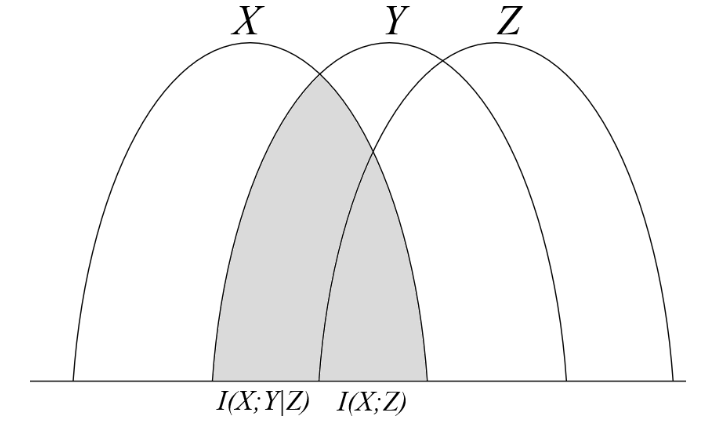
\includegraphics[height=4.5cm]{img/3-1.png}
          \caption{Venn Diagram of Exercise 1}
          \label{fig:ex1}
      \end{minipage}
      \begin{minipage}[t]{0.45\linewidth}
          \centering
          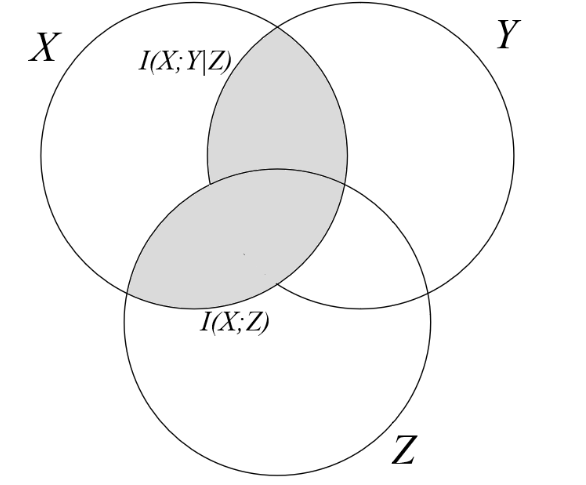
\includegraphics[height=4.5cm]{img/3-2.png}
          \caption{Venn Diagram of Exercise 2}
          \label{fig:ex2}
      \end{minipage}
\end{figure}


%%%%%%%%%%%%%%%%%%%%%%%%%%%%%%%%%%%%%%%%%%
%%%%%%%%%%%%%                 %%%%%%%%%%%%
%%%%%%%%%%%%%    EXERCISE 2   %%%%%%%%%%%%
%%%%%%%%%%%%%                 %%%%%%%%%%%%
%%%%%%%%%%%%%%%%%%%%%%%%%%%%%%%%%%%%%%%%%%
\begin{exercise}[]{Prove that the implication in Exercise \ref{ex1} continues to be valid without the Markov Chain constraint}
  \begin{proof}
    \begin{equation}
      \begin{array}{rll}
        I(X;Y) &= I(X;Y|Z) + (I(X;Y) - I(X;Y|Z)) & \text{(Note } X \bot Y|Z \rightarrow I(X;Y|Z) = 0 \text{)}\\[2mm]
        &= H(X) - H(X|Y) - (H(X|Z) - H(X|Y,Z)) & \text{(Fold by definition of mutual information)}\\[2mm]
        &= (H(X) - H(X|Z)) - (H(X|Y)- H(X|Y,Z)) & \text{(Unfold by definition of mutual information)}\\[2mm]
        &= I(X;Z) - I(X;Z|Y) &  \text{(Note } X \bot Y \rightarrow I(X;Y) = 0 \text{)} \\[2mm]
        &= - I(X;Z|Y) \le 0 & \text{(Nonnegative conditional mutual information)} 
      \end{array}
    \end{equation}
    On the other hand, $I(X;Y) \ge 0$. Hence $I(X;Y)$ must be zero. That is to say, $X \bot Y$.
  \end{proof}
  \end{exercise}

%%%%%%%%%%%%%%%%%%%%%%%%%%%%%%%%%%%%%%%%%%
%%%%%%%%%%%%%                 %%%%%%%%%%%%
%%%%%%%%%%%%%    EXERCISE 3   %%%%%%%%%%%%
%%%%%%%%%%%%%                 %%%%%%%%%%%%
%%%%%%%%%%%%%%%%%%%%%%%%%%%%%%%%%%%%%%%%%%
\begin{exercise}[]{Prove that $Y \bot Z|T$ implies $Y \bot Z|(X,T)$ conditioning on $X \rightarrow Y \rightarrow Z \rightarrow T$.}
  \begin{proof}
    \begin{equation}
      \begin{array}{rll}
        I(Y;Z|X,T) &= H(Y|X,T) - H(Y|Z,X,T) & \text{(Unfold mutual information)} \\[2mm]
        &= H(X,Y,T) - H(X,T) - H(X,Y,Z,T) + H(X,Z,T) & \text{(Unfold conditional entropy)} \\[2mm]
        &= (H(X,Y,T) - H(X,Y,Z,T)) - (H(X,T)-H(T)) &\\[2mm]
        & \quad + (H(X,Z,T)-H(Z,T)) -H(T) +H(Z,T) & \\[2mm]
        &= - H(Z|X,Y,T) - H(X|T) + H(X|Z,T) +H(Z|T) & \text{(Fold conditional entropy)} \\[2mm]
        &= (H(Z|T) - H(Z|Y,T)) - (H(X|T)-H(X|Z,T)) & \text{(Markov Chain: } p(z|x,y,t) = p(z|y,t) \text{)} \\[2mm]
        &= I(Y;Z|T) - I(X;Z|T) & \text{(Note } Y \bot Z|T \rightarrow I(Y;Z|T) = 0 \text{)} \\[2mm]
        &= - I(X;Z|T) \le 0  & \\[2mm]
      \end{array}
    \end{equation}
    On the other hand, $I(Y;Z|X,T) \ge 0$ can be proved by unfolding the definiton of conditional mutual information and the convexity property. Hence $I(Y;Z|X,T)$ must be zero. That is to say, $Y \bot Z|(X,T)$.
  \end{proof}
  \label{ex3}
  \end{exercise}

  \begin{figure}[htbp]
    \centering
        \begin{minipage}[t]{0.45\linewidth}
            \centering
            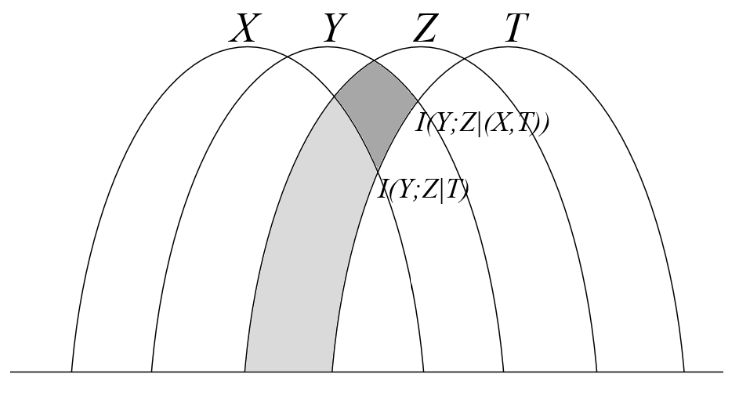
\includegraphics[height=4cm]{img/3-3.png}
            \caption{Venn Diagram of Exercise 3}
            \label{fig:ex3}
        \end{minipage}
        \begin{minipage}[t]{0.45\linewidth}
            \centering
            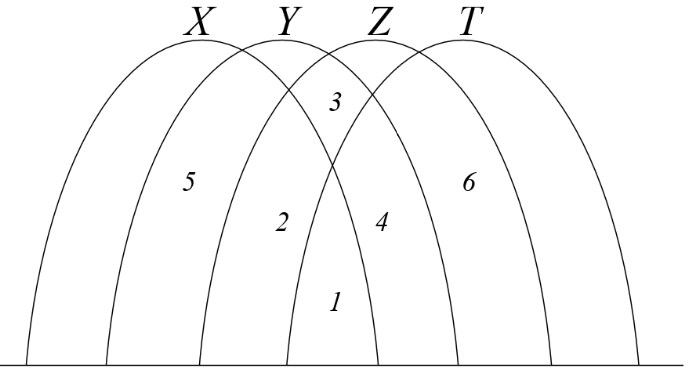
\includegraphics[height=4cm]{img/3-4.png}
            \caption{Venn Diagram of Exercise 4}
            \label{fig:ex4}
        \end{minipage}
  \end{figure}

%%%%%%%%%%%%%%%%%%%%%%%%%%%%%%%%%%%%%%%%%%
%%%%%%%%%%%%%                 %%%%%%%%%%%%
%%%%%%%%%%%%%    EXERCISE 4   %%%%%%%%%%%%
%%%%%%%%%%%%%                 %%%%%%%%%%%%
%%%%%%%%%%%%%%%%%%%%%%%%%%%%%%%%%%%%%%%%%%
\begin{exercise}[]{Let $X \rightarrow Y \rightarrow Z \rightarrow T$ form a Markov Chain. Determine which of the following always hold:
  \begin{enumerate}
    \item $I(X;T)+I(Y;Z) \ge I(X;Z)+I(Y;T)$
    \item $I(X;T)+I(Y;Z) \ge I(X;Y)+I(Z;T)$
    \item $I(X;Y)+I(Z;T) \ge I(X;Z)+I(Y;T)$
  \end{enumerate}
}
  \begin{solution}
    Inequality (1) and (3) always hold. We illustrate the answer through the venn diagram shown in Figure \ref{fig:ex4}, where area 1 $\sim$ 6 is respectively represented by $I(X;T),I(X;Z|T),I(Y;Z|(X,T)),I(Y;T|X),I(X;Y|Z),I(Z;T|Y)$.
    \begin{enumerate}
      \item {
        The inequality can be rewritten in form of areas as
        $$1+(1+2+3+4)\ge (1+2)+(1+4).$$
        Since $I(Y;Z|(X,T))\ge 0$, the inequality holds.
      }
      \item {
        The inequality can be rewritten in form of areas as
        $$1+(1+2+3+4)\ge (1+2+5)+(1+4+6).$$
        We can't determine the relation between $I(Y;Z|(X,T))$ (Area 3) and $I(X;Y|Z)+I(Z;T|Y)$ (Area 5 and 6) except that they are both nonnegative. The inequality will not always hold.
      }
      \item {
        The inequality can be rewritten in form of areas as
        $$(1+2+5)+(1+4+6)\ge (1+2)+(1+4).$$
        Since $I(X;Y|Z)+I(Z;T|Y) \ge 0$ can be proved by the nonnegativity of conditional mutual information, the inequality holds.
        Furthermore, the conclusion can also be derived from the data-processing inequality of Markov Chain with $I(X;Y)\ge I(X;Z)$ and $I(Z;T)\ge I(Y;T)$
      }
    \end{enumerate}
  \end{solution}
\end{exercise}



%%%%%%%%%%%%%%%%%%%%%%%%%%%%%%%%%%%%%%%%%%
%%%%%%%%%%%%%                 %%%%%%%%%%%%
%%%%%%%%%%%%%    EXERCISE 5   %%%%%%%%%%%%
%%%%%%%%%%%%%                 %%%%%%%%%%%%
%%%%%%%%%%%%%%%%%%%%%%%%%%%%%%%%%%%%%%%%%%
\begin{exercise}[Drawing with and without replacement]{An urn contains $r$ red, $w$ white, and $b$ black balls. Which has higher entropy, drawing $k \ge 2$ balls from the urn with replacement or without replacement? Set it up and show why. (There is both a difficult way and a relatively simple way to do this.)}
  \begin{solution}
    We use $X_i \in \left\{ \text{red, white, black} \right\}$ to identify the result of the i-th drawing. No matter with replacement or without replacement, the distributions of a single arbitrary variable $X_i$ are the same.
    \begin{equation}
      \begin{array}{cccc}
        X_i & red & white & black \\
        p(x) & \dfrac{r}{r+w+b} & \dfrac{w}{r+w+b} & \dfrac{b}{r+w+b} \\
      \end{array}
    \end{equation}

    With replacement, the previous result won't interfere with the present drawing. Hence we have $$H\left(X_{i} | X_{i-1}, \ldots, X_{1}\right)=H\left(X_{i}\right)$$. It follows that
    \begin{equation}
      H(X_1,X_2,...,X_k)  = \sum_{i=1}^{k}  H\left(X_{i} | X_{i-1}, \ldots, X_{1}\right) = \sum_{i=1}^{k}H\left(X_{i}\right) \quad \text{with replacement}
      \label{ex5:replace}
    \end{equation}

    Without replacement, we only have
    \begin{equation}
      H(X_1,X_2,...,X_k) = \sum_{i=1}^{k}  H\left(X_{i} | X_{i-1}, \ldots, X_{1}\right) \quad \text{without replacement}
      \label{ex5:noreplace}
    \end{equation}

    Note that in Equation \ref{ex5:replace} and Equation \ref{ex5:noreplace}, all the single-variable entropies are of the same value. By condition-reduce-entropy theorem we know that
    $$H\left(X_{i} | X_{i-1}, \ldots, X_{1}\right) \le H(X_i) \quad \text{for any } i $$

    Since the equality holds if and only if $X_i$ are mutually independent, which is not true in this problem, it follows that the entropy will be larger with replacement.
  \end{solution}
\end{exercise}

%%%%%%%%%%%%%%%%%%%%%%%%%%%%%%%%%%%%%%%%%%
%%%%%%%%%%%%%                 %%%%%%%%%%%%
%%%%%%%%%%%%%    EXERCISE 6   %%%%%%%%%%%%
%%%%%%%%%%%%%                 %%%%%%%%%%%%
%%%%%%%%%%%%%%%%%%%%%%%%%%%%%%%%%%%%%%%%%%
\begin{exercise}[Metric]{A function $\rho(x, y)$ is a metric if for all $x, y$,
  \begin{itemize}
    \setlength{\itemsep}{2pt}
    \setlength{\parsep}{0pt}
    \setlength{\parskip}{0pt}
    \item $\rho (x,y) \ge 0$.
    \item $\rho (x,y) = \rho (y,x)$.
    \item $\rho(x,y)=0$ if and only if $x=y$.
    \item $\rho(x,y)+\rho(y,z)\ge \rho(x,z)$.
  \end{itemize}
  \begin{enumerate}
    \item Show that $\rho(X, Y) = H(X|Y) + H(Y|X)$ satisfies the first, second, and fourth properties above. If we say that $X = Y$ if there is a one-to-one function mapping from X to Y, the third property is also satisfied, and $\rho(X, Y)$ is a metric.
    \item Verify that $\rho(X, Y)$ can also be expressed as
    \begin{equation}\begin{aligned}
      \rho(X, Y) &=H(X)+H(Y)-2 I(X ; Y) \\
      &=H(X, Y)-I(X ; Y) \\
      &=2 H(X, Y)-H(X)-H(Y)
      \end{aligned}\end{equation}
  \end{enumerate}
}
  \begin{proof}
    \par{~}
    \begin{enumerate}
      \item{
        \begin{itemize}
          \item Note that $H(X | Y) \geqslant 0 , \quad H(Y(X) \geqslant 0  \Rightarrow \quad \rho(X, Y) \geqslant 0$
          \item By unfolding the definition it's easy to see \(H(X | Y) \neq H(Y | X)=H(Y | X)+H(X | Y)\)
          \item If $X=Y$, there exists a one-to-one mapping, i.e. \(\rho(X,Y)= H(X | Y)+H(Y|X)=0\)
          
          On the other hand, if \(\rho(X,Y)= H(X | Y)+H(Y|X)=0\)
          Since $H(X | Y) \geqslant 0 , \quad H(Y(X) \geqslant 0$, we have $H(X | Y) = 0 , \quad H(Y(X) = 0$.
          By the conclusion in Exercise 2, Assignment 1, $X$ and $Y$ are mutually each other's function, i.e.there exists a one-to-one mapping between $X$ and $Y$.
          \item The conclusion can be derived using condition-reduce-entropy and nonnegativity of conditional entropy.
            \begin{equation}\begin{aligned}
            H(X | Y)+H(Y | X)+H(Y|Z)+H(Z | Y) & \geqslant H(X| Y,Z)+H(Y | X )+H(Y | Z)+H(Z | Y,X) \\
            &=H(X, Y | Z)+H(Z, Y | X) \\
            &=H(X | Z)+H(Y | X,Z)+H(Z | X)+H(Y | Z,X) \\
            &\geqslant H(X | Z)+H(Z | X)=\rho(X, Z)
            \end{aligned}\end{equation}
        \end{itemize}
        }
        \item {
          \begin{equation}\begin{aligned}
          \rho(X,Y)&=H(X | Y)+H(Y | X)&\\
          &=H(X)-I(X ; Y)+H(Y)-I(X ; Y) &\\
          &=H(X)+H(Y)-2 I(X ; Y) & (\star)\\
          &=(H(X)-I(X ; Y)+H(Y))-I(X ; Y)& \\
          &=H(X,Y)-I(X ; Y) & (\star)\\
          &=H(X,Y)-(H(X)+H(Y)-H(X,Y)) &\\
          &=2 H(X, Y)-H(X)-H(Y) & (\star)
          \end{aligned}\end{equation}
          The expressions required by the problem have been labeled with $(\star)$ in the derivation.
        }
      \end{enumerate}


  \end{proof}
  \end{exercise}

%%%%%%%%%%%%%%%%%%%%%%%%%%%%%%%%%%%%%%%%%%
%%%%%%%%%%%%%                 %%%%%%%%%%%%
%%%%%%%%%%%%%    EXERCISE 7   %%%%%%%%%%%%
%%%%%%%%%%%%%                 %%%%%%%%%%%%
%%%%%%%%%%%%%%%%%%%%%%%%%%%%%%%%%%%%%%%%%%
\begin{exercise}[Entropy of a disjoint mixture]{Let $X_1$ and $X_2$ be discrete random variables drawn according to probability mass functions $p_1(\cdot)$ and $p_2(\cdot)$ over the respective alphabets $X_1 = \left\{ 1, 2, \cdots , m \right\}$ and $X_2 = \left\{m + 1, \cdots , n\right\}$. Let
  \begin{equation}X=\left\{\begin{array}{ll}
    X_{1} & \text { with probability } \alpha \\
    X_{2} & \text { with probability } 1-\alpha
    \end{array}\right.\end{equation}
  \begin{enumerate}
    \item Find $H(X)$ in terms of $H(X_1), H(X_2)$ and $\alpha$.
    \item Maximize over $\alpha$ to show that $2^{H(X)} \le 2^{H(X_1)} + 2^{H(X_2)}$ and interpret using the notion that $2^{H(X)}$ is the effective alphabet
    size.
  \end{enumerate}
  }

  \begin{solution}
    \par{~}
    \begin{enumerate}
      \item {
        We calculate $H(X)$ by unfolding the definition of entropy.
        \begin{equation}
          \begin{aligned}
            H(X) &= - \sum_{x\in X_1} \alpha p_1 (x) \log \alpha p_1 (x) - \sum_{x\in X_2} (1-\alpha) p_2 (x) \log (1-\alpha) p_2 (x) \\
            &= - \alpha \log \alpha \sum_{x\in X_1} p_1 (x) - (1-\alpha) \log (1-\alpha) \sum_{x\in X_2} p_2 (x) + \alpha H(X_1) + (1-\alpha) H(X_2) \\
            &= - \alpha \log \alpha - (1-\alpha) \log (1-\alpha) + \alpha H(X_1) + (1-\alpha) H(X_2)
          \end{aligned}
        \end{equation}
      }
      \item {
        We consider $H(X)$ to be a function over $\alpha$. Note that $g(\alpha)= -\alpha\log(\alpha)$ is a concave function, and some affine transformation over $\alpha$ and linear components won't interfere with the concavity. The function of $H(x)$ is a concave function.

        We can get the maximal value by calculating the derivative of $H(X)$ over $\alpha$.
        \begin{equation}
          \begin{aligned}
            \frac{dH(X)}{d\alpha} &= - \frac{1}{d\alpha} \left(\frac{\alpha \ln \alpha}{\ln 2} + \frac{(1-\alpha)\ln(1-\alpha)}{\ln 2} - \alpha H(X_1) - (1-\alpha) H(X_2) \right) \\
            &= - \frac{1 + \ln \alpha}{\ln 2} - \frac{-1 - \ln(1-\alpha)}{\ln 2} + H(X_1) -H(X_2) := 0 \\
          \end{aligned}
        \end{equation}
        The maximal value is obtained at the derivative to be $0$.
        \begin{equation}
          \begin{aligned}
            -\ln \alpha + \ln (1-\alpha) &= \ln2 \left(H(X_2)-H(X_1)\right) \\
            \ln \frac{1-\alpha}{\alpha} &= \ln2 \left(H(X_2)-H(X_1)\right) \\
            \frac{1-\alpha}{\alpha} &= 2^{H(X_2)-H(X_1)} \\
            \alpha &= \frac{2^{H(X_1)}}{2^{H(X_2)}+2^{H(X_1)}}
          \end{aligned}
          \label{eqn:ex7}
        \end{equation}
        The optimal solution is in the domain, so the maximal value can be obtained. By substituting the $\alpha$ value into $2^{H(X)}$ we can obtain its upper bond.
        \begin{equation}
        \begin{aligned}
          2^{H(X)} &= 2^{- \alpha \log \alpha - (1-\alpha) \log (1-\alpha) + \alpha H(X_1) + (1-\alpha) H(X_2)} \\
          &= \alpha ^{-\alpha} \cdot (1-\alpha)^{\alpha - 1} \cdot \left(2^{H(X_1)}\right)^{\alpha} \cdot \left(2^{H(X_2)}\right)^{1-\alpha} \\
          &\le \left( \frac{2^{H(X_1)}}{2^{H(X_2)}+2^{H(X_1)}}\right) ^{-\alpha} \cdot \left( \frac{2^{H(X_2)}}{2^{H(X_2)}+2^{H(X_1)}}\right)^{\alpha - 1} \cdot \left(2^{H(X_1)}\right)^{\alpha} \cdot \left(2^{H(X_2)}\right)^{1-\alpha} \\
          &= \left(2^{H(X_1)}+2^{H(X_2)}\right) \cdot 2^{-\alpha H(X_1)} \cdot 2^{-(1-\alpha) H(X_2)}  \cdot \left(2^{H(X_1)}\right)^{\alpha} \cdot \left(2^{H(X_2)}\right)^{1-\alpha} \\
          &= 2^{H(X_1)}+2^{H(X_2)}
        \end{aligned}
        \end{equation}

        An interpretation of this conclusion is that $2^{H(X)}$ is the effective alphabet size of $X$, while $2^{H(X_1)}+2^{H(X_2)}$ is the sum sizes of the effective alphabets $X_1,X_2$. The alphabets of $X_1$ and $X_2$ do not overlap, with independent distribution, and they add up exactly to the alphabet of $X$. 

        If our probability of choice between $X_1$ and $X_2$ is in proportion to their effective alphabet size, as the third line in Equation \ref{eqn:ex7} shows, the resulting $X$ will have the effective alphabet size equivalent to the sum of $X_1$ and $X_2$.

        Otherwise, the unbalanced weight of $X_1$ and $X_2$ will reduce the actual effective alphabet size in $X$, since one variable's excessive occurence will reduce the occurence of the other, so that the latter's effective alphabet size will be less than what it really is.
      }
    \end{enumerate}
  \end{solution}
  \end{exercise}


%%%%%%%%%%%%%%%%%%%%%%%%%%%%%%%%%%%%%%%%%%
%%%%%%%%%%%%%                 %%%%%%%%%%%%
%%%%%%%%%%%%%    EXERCISE 8   %%%%%%%%%%%%
%%%%%%%%%%%%%                 %%%%%%%%%%%%
%%%%%%%%%%%%%%%%%%%%%%%%%%%%%%%%%%%%%%%%%%
\begin{exercise}[Entropy of a sum]{Let $X$ and $Y$ be random variables that take on values $x_1, x_2, \cdots , x_r$ and $y_1, \cdots, y_s$, respectively. Let $Z =
  X + Y$.
  \begin{itemize}
    \item Show that $H(Z|X) = H(Y|X)$. Argue that if $X, Y$ are independent, then $H(Y) \le H(Z)$ and $H(X) \le H(Z)$. Thus, the addition of independent random variables adds uncertainty.
    \item Give an example of (necessarily dependent) random variables in which $H(X) > H(Z)$ and $H(Y) > H(Z)$.
    \item Under what conditions does $H(Z) = H(X) + H(Y)$?
  \end{itemize}
}

\begin{solution}
  \par{~}
  \begin{enumerate}
    \item {
      $Z = X + Y$ indicates that any of the two variable can determine the third variable. That is to say, $$H(X|Y,Z)=H(Y|Z,X)=H(Z|X,Y) = 0$$. By observing $I(Y;Z|X)$ we have
      \begin{equation}
        \begin{aligned}
          I(Y;Z|X) &= H(Y|X) - H(Y|X,Z) \\
          &= H(Z|X) - H(Z|X,Y)
        \end{aligned}
      \end{equation}
      ,which implies that $H(Y|X)=H(Z|X)$.

      If $X$ and $Y$ are independent, $H(X,Y)=H(X)+H(Y)$.
      \begin{equation}
        \begin{aligned}
          H(X,Y,Z) &= H(Z|X,Y) + H(X,Y) = H(X)+H(Y)\\
          &= H(X|Y,Z)+H(Y,Z) = H(Z|X)+H(X) \\
          &= H(Y|X,Z)+H(X,Z) = H(Z|Y)+H(Y) \\
        \end{aligned}
        \label{eqn:ex8}
      \end{equation}

      Equation \ref{eqn:ex8} indicates that $H(Z|X)=H(Y)$ and that $H(Z|Y)=H(X)$. By condition-reduce-entropy theorem we have $H(Z) \ge H(Z|X)$ and $H(Z) \ge H(Z|Y)$. It follows that $H(Y) \le H(Z)$ and $H(X) \le H(Z)$.
    }
    \item {
      An exampling distribution of $X$ and $Y$ can be

      \begin{table}[H]
        \begin{center}  
          \begin{tabular}{|c|c|c|c|}
          \hline
          \multicolumn{2}{|c|}{\multirow{2}{*}{Prob}} & \multicolumn{2}{c|}{$x$}      \\ \cline{3-4} 
          \multicolumn{2}{|c|}{}                      & $0$           & $1$           \\ \hline
          \multirow{2}{*}{$y$}         & $0$          & $\frac{1}{2}$ & $0$           \\ \cline{2-4} 
                                      & $-1$         & $0$           & $\frac{1}{2}$ \\ \hline
          \end{tabular}
        \end{center}
      \end{table}

      The entropy of $X$ and $Y$ are 
      $$H(X)=H(Y) = \frac{1}{2}\log 2 + \frac{1}{2}\log 2 = 1$$
      The distribution of $Z=X+Y$ is $\Pr(Z=0) = 1$, which results in the entropy $H(Z) = 0 < H(X) = H(Y)$.    
    }

    \item {
      From $Z = X + Y$ we know $H(Z)=H(Z) - H(Z|X,Y) = I(X,Y;Z)$.

      $I(X,Y;Z) = H(X,Y)-H(X,Y|Z)$ indicates that $H(Z) \le H(X,Y)$. The equality holds if and only if $H(X,Y|Z) = 0$.
      
      Furthermore, $H(X,Y) = H(X) + H(Y) - I(X;Y)$, which implies that $H(X,Y)\le H(X) + H(Y)$. The equality holds if and only if $I(X;Y) = 0$, i.e. $X$ and $Y$ are independent.

      The second equality constraint and the propositions that $H(X|Y,Z)=H(Y|Z,X) = 0$ can ensure the first equality constraint. Therefore, under the condition that $X$ and $Y$ are independent will $H(Z) = H(X) + H(Y)$ hold.
    }
  \end{enumerate}
\end{solution}
\end{exercise}

%%%%%%%%%%%%%%%%%%%%%%%%%%%%%%%%%%%%%%%%%%
%%%%%%%%%%%%%                 %%%%%%%%%%%%
%%%%%%%%%%%%%    EXERCISE 9   %%%%%%%%%%%%
%%%%%%%%%%%%%                 %%%%%%%%%%%%
%%%%%%%%%%%%%%%%%%%%%%%%%%%%%%%%%%%%%%%%%%
\begin{exercise}[Data processing]{Let $X_1 \rightarrow X_2\rightarrow  X_3 \rightarrow \cdots \rightarrow X_n$ form a Markov chain in this order; that is, let
  $$p\left(x_{1}, x_{2}, \ldots, x_{n}\right)=p\left(x_{1}\right) p\left(x_{2} | x_{1}\right) \cdots p\left(x_{n} | x_{n-1}\right)$$

  Reduce $I(X_1;X_2, \cdots , X_n)$ to its simplest form.
  }

  \begin{solution}
    By the chain rule of mutual information we have
    $$I\left(X_{1}; X_{2}, \ldots, X_{n}\right) =\sum_{i=2}^{n} I\left(X_{i} ;  X_1 | X_{i-1}, X_{i-2}, \ldots, X_{2}\right) $$
    Note that for $i>2$, we have
    \begin{equation}
      \begin{aligned}
        I\left(X_{i} ;  X_1 | X_{i-1}, X_{i-2}, \ldots, X_{2}\right) &= H\left(X_i|X_{i-1}, X_{i-2}, \ldots, X_{2}\right ) - H\left(X_i|X_{i-1}, X_{i-2}, \ldots, X_{2}, X_{1}\right ) \\
        &= H(X_i|X_{i-1}) - H(X_i|X_{i-1}) = 0 \quad \text{(Markov Chain)}
      \end{aligned}
    \end{equation}
    It follows that $I\left(X_{1}; X_{2}, \ldots, X_{n}\right) =  I\left(X_{1} ;  X_2 \right) $.


  \end{solution}
\end{exercise}


%%%%%%%%%%%%%%%%%%%%%%%%%%%%%%%%%%%%%%%%%%
%%%%%%%%%%%%%                 %%%%%%%%%%%%
%%%%%%%%%%%%%    EXERCISE 10  %%%%%%%%%%%%
%%%%%%%%%%%%%                 %%%%%%%%%%%%
%%%%%%%%%%%%%%%%%%%%%%%%%%%%%%%%%%%%%%%%%%
\begin{exercise}[Infinite entropy]{This problem shows that the entropy of a discrete random variable can be infinite. Let $A = \sum_{n=2}^{\infty} (n \log^{2} n)^{-1}$. [It is easy to show that $A$ is finite by bounding the infinite sum by the integral of $(x \log^{2} x)^{-1}$. ] Show that the integer-valued random variable $X$ defined by $\text{Pr}(X = n) = (An \log^2 n)^{-1}$ for $n = 2, 3, \cdots,$ has $H(X) = +\infty$.}

  \begin{proof}
    By definition of entropy we can calculate that
    \begin{equation}
      \begin{aligned}
        H(X) &= - \sum_{n = 2}^{\infty} p(n)\log p(n) \\
        &= \sum_{n=2}^{\infty} (An\log^2 n)^{-1} \log (An\log^2 n) \\
        &= \sum_{n=2}^{\infty} \frac{\log A + \log n + \log^2 n}{An\log^2 n} \\
        &= \log A + \sum_{n=2}^{\infty} \frac{1}{An\log n} + \sum_{n=2}^{\infty} \frac{\log^2 n}{An\log^2 n} \\
      \end{aligned}
    \end{equation}
    As has been indicated by the condition, the first component is finite. The last component will be nonnegative with sufficiently large $n$. We show that the second component is infinite. Note that
    $$0 <  \sum_{n=2}^{\infty} \frac{1}{An\log n} < \int_{2}^{\infty} \frac{\ln 2 dx}{A x \ln x} = \int_{2}^{\infty} \frac{\ln 2 d(\ln x)}{A \ln x} = \frac{\ln 2}{A} \ln(\ln x) \bigg|_{2}^{\infty} \rightarrow \infty$$
    It follows that $H(X)=+\infty$
  \end{proof}
\end{exercise}

\section{Entropy Rate}
%%%%%%%%%%%%%%%%%%%%%%%%%%%%%%%%%%%%%%%%%%
%%%%%%%%%%%%%                 %%%%%%%%%%%%
%%%%%%%%%%%%%    EXERCISE 1   %%%%%%%%%%%%
%%%%%%%%%%%%%                 %%%%%%%%%%%%
%%%%%%%%%%%%%%%%%%%%%%%%%%%%%%%%%%%%%%%%%%
\begin{exercise}[Monotonicity of entropy per element]{For a stationary stochastic process $X_{1}, X_{2}, \ldots, X_{n},$ show that
  $$
  \begin{aligned}
  \frac{H\left(X_{1}, X_{2}, \ldots, X_{n}\right)}{n} & \leq \frac{H\left(X_{1}, X_{2}, \ldots, X_{n-1}\right)}{n-1} \\
  \frac{H\left(X_{1}, X_{2}, \ldots, X_{n}\right)}{n} & \geq H\left(X_{n} | X_{n-1}, \ldots, X_{1}\right)
  \end{aligned}
  $$}
  \begin{proof}
  \par{~}

  We first prove the second statement by properties of stationary process.

  \begin{equation}\begin{aligned}
    H\left(X_{1}, \cdots, X_{n}\right) &=\sum_{i=1}^{n} H\left(X_{i} | X_{i-1}, \cdots X_{2}, X_{1}\right) \\
    & \geqslant \sum_{i=1}^{n} H\left(X_{i} | X_{i-1}, X_{i-2}, \cdots, X_{n-i+1}\right) \\
    &=\sum_{i=1}^{n} H\left(X_{n} | X_{n-1}, \cdots, X_{2}, X_{1}\right) \\
    &=n H\left(X_{n} | X_{1}, X_{2}, \cdots, X_{n-1}\right)
    \end{aligned}\label{eqn:ex1}\end{equation}

    By Equation \ref{eqn:ex1} and entropy equalities we can prove the first statement.

  \begin{equation}\begin{aligned}
    (n-1) H\left(X_{1}, \cdots, X_{n}\right) & \leqslant n H\left(X_{1}, \cdots, X_{n}\right)-H\left(X_{1}, \cdots, X_{n}\right) \\
    & \leqslant n\left[H\left(X_{1}, \cdots, X_{n}\right)-H\left(X_{n}|X_{1}, \cdots, X_{n-1}\right)\right]\\
    &=n H\left(X_{1}, \cdots, X_{n-1}\right)
    \end{aligned}\end{equation}


  \end{proof}
  \label{ex1}
\end{exercise}

%%%%%%%%%%%%%%%%%%%%%%%%%%%%%%%%%%%%%%%%%%
%%%%%%%%%%%%%                 %%%%%%%%%%%%
%%%%%%%%%%%%%    EXERCISE 2   %%%%%%%%%%%%
%%%%%%%%%%%%%                 %%%%%%%%%%%%
%%%%%%%%%%%%%%%%%%%%%%%%%%%%%%%%%%%%%%%%%%
\begin{exercise}[Initial conditions]{ Show, for a Markov chain, that
  $$
  H\left(X_{0} | X_{n}\right) \geq H\left(X_{0} | X_{n-1}\right)
  $$
  Thus, initial conditions $X_{0}$ become more difficult to recover as the future $X_{n}$ unfolds.}
  \begin{proof}
  For Markov Chain, we have $p(x_0|x_n,x_{n-1}) = p(x_0|x_{n-1})$. Hence
  \begin{equation}
    \begin{aligned}
      H(X_0|X_n,X_{n-1}) &= -\sum_{x_n,x_{n-1}} p(x_n,x_{n-1}) \sum_{x_0} p(x_0|x_n,x_{n-1}) \log    p(x_0|x_n,x_{n-1}) \\
      &= -\sum_{x_{n-1}} \left( \sum_{x_{n}} p(x_n,x_{n-1}) \right) \sum_{x_0} p(x_0|x_{n-1}) \log    p(x_0|x_{n-1})\\
      &= -\sum_{x_{n-1}} p(x_{n-1}) \sum_{x_0} p(x_0|x_{n-1}) \log    p(x_0|x_{n-1}) = H(X_0|X_{n-1})
    \end{aligned}
  \end{equation}
  Since condition reduce entropy, we have $  H(X_0|X_{n-1}) = H(X_0|X_n,X_{n-1}) \le  H(X_0|X_n) $
  \end{proof}
  \label{ex2}
\end{exercise}

%%%%%%%%%%%%%%%%%%%%%%%%%%%%%%%%%%%%%%%%%%
%%%%%%%%%%%%%                 %%%%%%%%%%%%
%%%%%%%%%%%%%    EXERCISE 3   %%%%%%%%%%%%
%%%%%%%%%%%%%                 %%%%%%%%%%%%
%%%%%%%%%%%%%%%%%%%%%%%%%%%%%%%%%%%%%%%%%%
\begin{exercise}[The past has little to say about the future]{For a stationary stochastic process $X_{1}, X_{2}, \ldots, X_{n}, \ldots,$ show that
  $$
  \lim _{n \rightarrow \infty} \frac{1}{2 n} I\left(X_{1}, X_{2}, \ldots, X_{n} ; X_{n+1}, X_{n+2}, \ldots, X_{2 n}\right)=0
  $$}
  \begin{proof} First Note that
    \begin{equation}
      I\left(X_{1}, X_{2}, \ldots, X_{n} ; X_{n+1}, X_{n+2}, \ldots, X_{2 n}\right) = H(X_1,\ldots,X_n) - H(X_{n+1},\ldots,X_{2n}|X_1,\ldots,X_n)
    \end{equation}
    By definition of entropy rate we know that $$\frac{1}{2}\sum_{i=1}^{n} H(X_1,\ldots,X_n) \rightarrow H(\mathcal{X})$$



  \end{proof}
  \label{ex3}
\end{exercise}


%%%%%%%%%%%%%%%%%%%%%%%%%%%%%%%%%%%%%%%%%%
%%%%%%%%%%%%%                 %%%%%%%%%%%%
%%%%%%%%%%%%%    EXERCISE 4   %%%%%%%%%%%%
%%%%%%%%%%%%%                 %%%%%%%%%%%%
%%%%%%%%%%%%%%%%%%%%%%%%%%%%%%%%%%%%%%%%%%
\begin{exercise}[Entropy rate]{ Let $\left\{X_{i}\right\}$ be a discrete stationary stochastic process with entropy rate $H(\mathcal{X}) .$ Show that
  $$
  \frac{1}{n} H\left(X_{n}, \ldots, X_{1} | X_{0}, X_{-1}, \ldots, X_{-k}\right) \rightarrow H(\mathcal{X})
  $$
  for $k=1,2, \ldots$}
  \begin{proof}
  \begin{equation}
      H\left(X_{n}, \ldots, X_{1} | X_{0}, X_{-1}, \ldots, X_{-k}\right) = \sum_{i=1}^{n} H(X_i|X_{i-1},\ldots,X_{-k})
  \end{equation}
  Note that $$H'(X) = \lim_{n\rightarrow \infty}H(X_n|X_{n-1},ldots,X_1) = \lim_{n\rightarrow \infty}H(X_n|X_{n-1},\ldots,X_{-k})$$
  We already know that $H'(X)\rightarrow H(\mathcal{X})$.

  By Cesaro Mean, $$
  \frac{1}{n} H\left(X_{n}, \ldots, X_{1} | X_{0}, X_{-1}, \ldots, X_{-k}\right) \rightarrow H(\mathcal{X})
  $$
  \end{proof}
  \label{ex4}
\end{exercise}


%%%%%%%%%%%%%%%%%%%%%%%%%%%%%%%%%%%%%%%%%%
%%%%%%%%%%%%%                 %%%%%%%%%%%%
%%%%%%%%%%%%%    EXERCISE 5   %%%%%%%%%%%%
%%%%%%%%%%%%%                 %%%%%%%%%%%%
%%%%%%%%%%%%%%%%%%%%%%%%%%%%%%%%%%%%%%%%%%
\begin{exercise}[Markov’s inequality and Chebyshev’s inequality]{\par{~}
  \begin{enumerate}
    \item (Markov's inequality) For any nonnegative random variable $X$ and any $t>0,$ show that\begin{equation}\operatorname{Pr}\{X \geq t\} \leq \frac{E X}{t}\end{equation} Exhibit a random variable that achieves this inequality with equality. 
    \item (Chebyshev's inequality) Let $Y$ be a random variable with mean $\mu$ and variance $\sigma^{2} .$ By letting $X=(Y-\mu)^{2},$ show that for any $\epsilon>0$
    \begin{equation}
      \operatorname{Pr}\{|Y-\mu|>\epsilon\} \leq \frac{\sigma^{2}}{\epsilon^{2}}
    \end{equation}
    \item (Weak law of large numbers) Let $Z_{1}, Z_{2}, \ldots, Z_{n}$ be a sequence of i.i.d. random variables with mean $\mu$ and variance $\sigma^{2} .$ Let $\bar{Z}_{n}=\frac{1}{n} \sum_{i=1}^{n} Z_{i}$ be the sample mean. Show that
  \begin{equation}\operatorname{Pr}\left\{\left|\bar{Z}_{n}-\mu\right|>\epsilon\right\} \leq \frac{\sigma^{2}}{n \epsilon^{2}}\end{equation}
    Thus, $\operatorname{Pr}\left\{\left|\bar{Z}_{n}-\mu\right|>\epsilon\right\} \rightarrow 0$ as $n \rightarrow \infty .$ This is known as the weak law of large numbers.
  \end{enumerate}}
  \begin{proof}
  \par{~}
  \begin{enumerate}
    \item {
      Note that for any $t$,
      \begin{equation}
        t \cdot 1_{\left\{X\ge t\right\}} \le X
      \end{equation}
      By taking expectation at both sides we have
      \begin{equation}
        E(1_{\left\{X\ge t\right\}}) = \Pr (X\ge t) \le \frac{EX}{t}
      \end{equation}
    }
    \item {
      Note $EX = DY =\sigma^2$. By letting $X = (Y-\mu)^2$ and $t = \epsilon^2$ in the Markov inequality, we can derive that
    \begin{equation}\operatorname{Pr}\left\{\left|\bar{Z}_{n}-\mu\right|>\epsilon\right\} \leq \frac{\sigma^{2}}{n \epsilon^{2}}\end{equation}
    }
    \item {
      Note $E\bar{Z_n} = \mu$ and $D\bar{Z_n} = \frac{1}{n^2} \sum_{i=1}^n DZ_i = \frac{\sigma^2}{n}$. By applying Chebyshev's inequality on $\bar{Z_n}$ we have
    \begin{equation}\operatorname{Pr}\left\{\left|\bar{Z}_{n}-\mu\right|>\epsilon\right\} \leq \frac{\sigma^{2}}{n \epsilon^{2}}\end{equation}
    }
  \end{enumerate}
  \end{proof}
  \label{ex5}
\end{exercise}

%%%%%%%%%%%%%%%%%%%%%%%%%%%%%%%%%%%%%%%%%%
%%%%%%%%%%%%%                 %%%%%%%%%%%%
%%%%%%%%%%%%%    EXERCISE 6   %%%%%%%%%%%%
%%%%%%%%%%%%%                 %%%%%%%%%%%%
%%%%%%%%%%%%%%%%%%%%%%%%%%%%%%%%%%%%%%%%%%
\begin{exercise}[Piece of cake]{ A cake is sliced roughly in half, the largest piece being chosen each time, the other pieces discarded. We will assume that a random cut creates pieces of proportions
  $$
  P=\left\{\begin{array}{ll}
  \left(\frac{2}{3}, \frac{1}{3}\right) & \text { with probability } \frac{3}{4} \\
  \left(\frac{2}{5}, \frac{3}{5}\right) & \text { with probability } \frac{1}{4}
  \end{array}\right.
  $$
  Thus, for example, the first cut (and choice of largest piece) may result in a piece of size $\frac{3}{5} .$ Cutting and choosing from this piece might reduce it to size $\left(\frac{3}{5}\right)\left(\frac{2}{3}\right)$ at time $2,$ and so on. How large, to first order in the exponent, is the piece of cake after $n$ cuts?}
  \begin{solution}
  Let $C_1, C_2, \ldots, C_n$ denote the choice of each cut. Then after $n$ cuts, the size of the cake $W_n = \prod_{i=1}^n C_i$. By taking the logarithm at the equation, we have $\log W_n = \sum_{i=1}^n \log C_i$. Since $C_i$s are i.i.d., we can apply the law of large numbers as follows.
  \begin{equation}
    \lim_{n\rightarrow\infty}\frac{1}{n} \log W_n = E(\log C) = \frac{3}{4}\log \frac{2}{3} + \frac{1}{4} \log \frac{3}{5} \approx -0.494
  \end{equation}
  Note that the equation above indicates that
  \begin{equation}
    \begin{aligned}
      \frac{1}{n} \log W_n &= -0.494 + o(1)
      W_n &= 2^{-0.494t +o(n)}
    \end{aligned}
  \end{equation}
  So the first order in the exponent is $\frac{3}{4}\log \frac{2}{3} + \frac{1}{4} \log \frac{3}{5} \approx -0.494$.
  \end{solution}
  \label{ex6}
\end{exercise}

%%%%%%%%%%%%%%%%%%%%%%%%%%%%%%%%%%%%%%%%%%
%%%%%%%%%%%%%                 %%%%%%%%%%%%
%%%%%%%%%%%%%    EXERCISE 7   %%%%%%%%%%%%
%%%%%%%%%%%%%                 %%%%%%%%%%%%
%%%%%%%%%%%%%%%%%%%%%%%%%%%%%%%%%%%%%%%%%%
\begin{exercise}[AEP]{ Let $X_{i}$ be iid $\sim p(x), x \in\{1,2, \ldots, m\} .$ Let $\mu=E X$ and $H=-\sum p(x) \log p(x) .$ Let $A^{n}=\left\{x^{n} \in \mathcal{X}^{n}: |-\frac{1}{n} \log p\left(x^{n}\right)-\right.$
  $H | \leq \epsilon\} .$ Let $B^{n}=\left\{x^{n} \in \mathcal{X}^{n}:\left|\frac{1}{n} \sum_{i=1}^{n} X_{i}-\mu\right| \leq \epsilon\right\}$
  \begin{enumerate}
    \item Does $\operatorname{Pr}\left\{X^{n} \in A^{n}\right\} \longrightarrow 1 ?$
    \item Does $\operatorname{Pr}\left\{X^{n} \in A^{n} \cap B^{n}\right\} \longrightarrow 1 ?$
    \item Show that $\left|A^{n} \cap B^{n}\right| \leq 2^{n(H+\epsilon)}$ for all $n$
    \item Show that $\left|A^{n} \cap B^{n}\right| \geq\left(\frac{1}{2}\right) 2^{n(H-\epsilon)}$ for $n$ sufficiently large.
  \end{enumerate}}
  \begin{solution}
  \par{~}
  \begin{enumerate}
    \item {
      Yes. By the Large Number Law,
      \begin{equation}
        - \frac{1}{n}\log p(x^n) = - \frac{1}{n} \sum_{i=1}^{n} \log p(X_i) \rightarrow H(X) \text{\quad in probability}
      \end{equation}
      , which implies that
      \begin{equation}
        \Pr \left\{X^n \in A^n \right\} = \Pr \left\{ | -\frac{1}{n} \log p\left(x^{n}\right)-H | \leq \epsilon \right\} \rightarrow 1
      \end{equation}
      }
    \item {
      Yes. Part (1) implies that $\lim_{n\rightarrow\infty} \Pr \left\{X^n \in A^n \right\} = 1$.

      By strong law of large number we have $\lim_{n\rightarrow\infty} \Pr \left\{X^n \in B^n \right\} = 1$

      For arbitrary $\delta > 0$, there exists $N_1$, such that  $\Pr \left\{X^n \in A^n \right\} > 1 - \frac{\delta}{2}$ for all $n>N_1$, and there exists $N_2$, such that  $\Pr \left\{X^n \in B^n \right\} > 1 - \frac{\delta}{2}$ for all $n>N_2$.
      We take $N = \max \left\{N_1,N_2\right\}$, for any $n>N$, we have
      \begin{equation}
        \begin{aligned}
          \Pr \left\{X^{n} \in A^{n} \cap B^{n}\right\} &= \Pr \left\{X^n \in A^n \right\} +  \Pr \left\{X^n \in B^n \right\} - \Pr \left\{X^n \in A^n \cup B^n \right\}\\
          & > 1 - \frac{\delta}{2} + 1 - \frac{\delta}{2} - 1 = 1 - \delta
        \end{aligned}
      \end{equation}
      , which indicates that $\Pr \left\{X^{n} \in A^{n} \cap B^{n}\right\} \rightarrow 1$
    }
    \item {
      From $x^n\in A^n$ we know that
      \begin{equation}
        2^{-n(H+\epsilon)} \le p(x^n) \le 2^{-n(H-\epsilon)}
      \end{equation}
      \begin{equation}
        \begin{aligned}
          1 &= \sum_{x^n\in \mathcal{x}^n} p(x) \\
          &\ge \sum_{x^n\in A^n \cap B^n} p(x) \\
          &\ge 2^{-n(H(X)+\epsilon)} |A^n\cap B^n|
        \end{aligned}
      \end{equation}
      It follows that $\left|A^{n} \cap B^{n}\right| \leq 2^{-n(H+\epsilon)}$.
    }
    \item {
      From $\Pr \left\{X^n \in A^n \cap B^n \right\} \rightarrow 1$, we take $\delta = \frac{1}{2}$, then there exists sufficiently large $n$, such that
      \begin{equation}
        \begin{aligned}
          \frac{1}{2} &\le \Pr (X^n \in A^n \cap B^n) \\
          &\le \sum_{x^n \in A^n \cap B^n} p(x^n) \\
          &\le |A^n\cap B^n| 2^{-n(H(X)-\epsilon)}
        \end{aligned}
      \end{equation}
      It follows that $\left|A^{n} \cap B^{n}\right| \geq \left( \frac{1}{2}\right) 2^{-n(H-\epsilon)}$.
    }
  \end{enumerate}
  \end{solution}
  \label{ex7}
\end{exercise}

%%%%%%%%%%%%%%%%%%%%%%%%%%%%%%%%%%%%%%%%%%
%%%%%%%%%%%%%                 %%%%%%%%%%%%
%%%%%%%%%%%%%    EXERCISE 8   %%%%%%%%%%%%
%%%%%%%%%%%%%                 %%%%%%%%%%%%
%%%%%%%%%%%%%%%%%%%%%%%%%%%%%%%%%%%%%%%%%%
\begin{exercise}[Doubly stochastic matrices]{$\quad$ An $n \times n$ matrix $P=\left[P_{i j}\right]$ is said to be doubly stochastic if $P_{i j} \geq 0$ and $\sum_{j} P_{i j}=1$ for all $i$ and $\sum_{i} P_{i j}=1$ for all $j .$ An $n \times n$ matrix $P$ is said to be a permutation matrix if it is doubly stochastic and there is precisely one $P_{i j}=1$ in each row and each column. It can be shown that every doubly stochastic matrix can be written as the convex combination of permutation matrices.
  \begin{enumerate}
    \item Let $\mathbf{a}^{t}=\left(a_{1}, a_{2}, \ldots, a_{n}\right), a_{i} \geq 0, \sum a_{i}=1,$ be a probability vector. Let $\mathbf{b}=\mathbf{a} P,$ where $P$ is doubly stochastic. Show that $\mathbf{b}$ is a probability vector and that $H\left(b_{1}, b_{2}, \ldots, b_{n}\right) \geq H\left(a_{1}, a_{2}, \ldots, a_{n} \right)$. Thus, stochastic mixing increases entropy.
    \item Show that a stationary distribution $\mu$ for a doubly stochastic matrix $P$ is the uniform distribution.
    \item Conversely, prove that if the uniform distribution is a stationary distribution for a Markov transition matrix $P,$ then $P$ is doubly stochastic.
  \end{enumerate}}
  \begin{proof}
  \par{~}
  \begin{enumerate}
    \item {
      From $\mathbf{b} = \mathbf{a}P$ we know that
      \begin{equation}
        b_j = \sum_{i=1}^{m} a_i p_{ij}
      \end{equation}
      Then we have.
      \begin{equation}
        \begin{aligned}
          H(\mathbf{b}) - H(\mathbf{a}) &= - \sum_{j=1}^{m} \left(\sum_{i=1}^{m} a_i p_{ij}\right) \log  b_j + \sum_{i=1}^{m} a_i \log a_i \\
          &= - \sum_{i=1}^{m} a_i \left(\sum_{j=1}^{m} p_{ij}\log  b_j \right)+ \sum_{i=1}^{m} a_i \left(\sum_{j=1}^{m} p_{ij} \log a_i \right) \\
          &= \sum_{i=1}^{m} \sum_{j=1}^{m} a_i  p_{ij}\log \frac{a_i}{b_j} \\
          &= \sum_{i=1}^{m} \sum_{j=1}^{m} b_j  p_{ij} \left(\frac{a_i}{b_j} \log \frac{a_i}{b_j} \right) \\
          &\ge \left(\sum_{i=1}^{m} \sum_{j=1}^{m} b_j  p_{ij} \frac{a_i}{b_j} \right) \log \left(\sum_{i=1}^{m} \sum_{j=1}^{m} b_j  p_{ij} \frac{a_i}{b_j} \right) \\
          &= \left(\sum_{i=1}^{m} \sum_{j=1}^{m} p_{ij} a_i\right) \log \left(\sum_{i=1}^{m} \sum_{j=1}^{m} p_{ij} a_i\right) = 1 \cdot \log 1 = 0
        \end{aligned}
      \end{equation}
    }
    \item {
     By condition we have $\mu_i = \frac{1}{m}$ for any $i$. Since for any $j$, 
     \begin{equation}
      \sum_{i=1}^{m} \mu_i p_{ij} = \frac{1}{m} \sum_{i=1}^{m} p_{ij} = \frac{1}{m} = \mu_i
     \end{equation}
     We have that $\mathbf{\mu} P = \mathbf{\mu}$. The uniform distribution is a stationary distribution for a doubly stochastic matrix.
    }
    \item {
      From $\mathbf{\mu} P = \mathbf{\mu}$ and $\mu = \frac{1}{m}$, we know that
      \begin{equation}
        \sum_{i=1}^{m} \frac{1}{m} p_{ij} = \frac{1}{m}
       \end{equation}
      holds for any $j$, which implies
      \begin{equation}
        \sum_{i=1}^{m} p_{ij} = 1 \text{\quad for any} j
      \end{equation}
      Then $P$ is doubly stochastic.
    }
  \end{enumerate}
  \end{proof}
  \label{ex8}
\end{exercise}

%%%%%%%%%%%%%%%%%%%%%%%%%%%%%%%%%%%%%%%%%%
%%%%%%%%%%%%%                 %%%%%%%%%%%%
%%%%%%%%%%%%%    EXERCISE 9   %%%%%%%%%%%%
%%%%%%%%%%%%%                 %%%%%%%%%%%%
%%%%%%%%%%%%%%%%%%%%%%%%%%%%%%%%%%%%%%%%%%
\begin{exercise}[Shuffes increase entropy]{ Argue that for any distribution on shuffles $T$ and any distribution on card positions $X$ that
  $$
  \begin{aligned}
  H(T X) & \geq H(T X | T) \\
  &=H\left(T^{-1} T X | T\right) \\
  &=H(X | T) \\
  &=H(X)
  \end{aligned}
  $$
  if $X$ and $T$ are independent.}
  \begin{proof} The first line holds because condition reduces entropy. The second line holds since $T^{-1}$ can be given by the condition $T$. The last line holds if $X$ and $T$ are independent, which finishes the proof.
  \end{proof}
  \label{ex9}
\end{exercise}

%%%%%%%%%%%%%%%%%%%%%%%%%%%%%%%%%%%%%%%%%%
%%%%%%%%%%%%%                 %%%%%%%%%%%%
%%%%%%%%%%%%%    EXERCISE 10  %%%%%%%%%%%%
%%%%%%%%%%%%%                 %%%%%%%%%%%%
%%%%%%%%%%%%%%%%%%%%%%%%%%%%%%%%%%%%%%%%%%
\begin{exercise}[Entropy rates of Markov chains]{ \par{~}
  \begin{enumerate}
    \item Find the entropy rate of the two-state Markov chain with transition matrix
    $$
    P=\left[\begin{array}{cc}
    1-p_{01} & p_{01} \\
    p_{10} & 1-p_{10}
    \end{array}\right]
    $$
    \item What values of $p_{01}, p_{10}$ maximize the entropy rate?
    \item Find the entropy rate of the two-state Markov chain with transition matrix
    $$
    P=\left[\begin{array}{cc}
    1-p & p \\
    1 & 0
    \end{array}\right]
    $$
    \item Find the maximum value of the entropy rate of the Markov chain of part (c). We expect that the maximizing value of $p$ should be less than $\frac{1}{2},$ since the 0 state permits more information to be generated than the 1 state.
    \item Let $N(t)$ be the number of allowable state sequences of length $t$ for the Markov chain of part (c). Find $N(t)$ and calculate
    $$
    H_{0}=\lim _{t \rightarrow \infty} \frac{1}{t} \log N(t)
    $$
  \end{enumerate}
  [Hint: Find a linear recurrence that expresses $N(t)$ in terms of $N(t-1)$ and $N(t-2) .$ Why is $H_{0}$ an upper bound on the entropy rate of the Markov chain? Compare $H_{0}$ with the maximum entropy found in part (d). $]$}
  \begin{solution}
  \par{~}
  \begin{enumerate}
    \item {
      We first calculate the stationary distribution $\mathbf{\mu}$.
      \begin{equation}
        \left\{\begin{array}{c}
          \mathbf{\mu}P = \mathbf{\mu} \\
          \mathbf{\mu} \mathbf{1}^T = 1
        \end{array}\right. \Rightarrow \mu = \left[\frac{p_{10}}{p_{01}+p_{10}}, \frac{p_{01}}{p_{01}+p_{10}}\right]
      \end{equation}
      By the entropy rate of Markov Chain,
      \begin{equation}
        \begin{aligned}
          H(\mathcal{X}) &= \sum_{i=1,2} \mu_i \left(\sum_{j=1,2} - p_{ij} \log {p_{ij}}\right) \\
          &= \frac{p_{10}H(p_{01})+p_{01}H(p_{10})}{p_{01}+p_{10}}
        \end{aligned}
      \end{equation}
    }
    \item {
      Note that the entropy is upper bounded by its alphabet, since
      \begin{equation}
        \frac{1}{n} H\left(X_{1}, X_{2}, \ldots, X_{n}\right) \le \frac{1}{n} \log |\mathcal{X}|^n = \log |\mathcal{X}|
      \end{equation}
      Hence the maximal entropy rate for this problem is $\log 2 = 1$. This can be obtained when $p_{01} = p_{10} = \frac{1}{2}$, where
      \begin{equation}
        \begin{aligned}
          H(\mathcal{X}) &= \frac{p_{10}H(p_{01})+p_{01}H(p_{10})}{p_{01}+p_{10}} \\
          &= \frac{1}{2} + \frac{1}{2}  = 1
        \end{aligned}
      \end{equation}
      Therefore, $p_{01} = p_{10} = \frac{1}{2}$ maximize the entropy rate.
    }
    \item {
      We first calculate the stationary distribution $\mathbf{\mu}$.
      \begin{equation}
        \left\{\begin{array}{c}
          \mathbf{\mu}P = \mathbf{\mu} \\
          \mathbf{\mu} \mathbf{1}^T = 1
        \end{array}\right. \Rightarrow \mu = \left[\frac{1}{p+1}, \frac{p}{p+1}\right]
      \end{equation}
      By the entropy rate of Markov Chain,
      \begin{equation}
        \begin{aligned}
          H(\mathcal{X}) &= \sum_{i=1,2} \mu_i \left(\sum_{j=1,2} - p_{ij} \log {p_{ij}}\right) \\
          &= \frac{-p\log p -(1-p)\log (1-p)}{p+1}
        \end{aligned}
      \end{equation}
    }
    \item { We take the derivative of $H(\mathcal{X})$.
    \begin{equation}
        \frac{d H(\mathcal{X})}{dp} = \frac{\log(1-p) -\log p+\log(1-p)}{(p+1)^2} := 0 \quad 
        \Rightarrow \quad p =  \frac{3- \sqrt{5}}{2}
    \end{equation}
    The maximal entropy rate is $\log \frac{1+\sqrt{5}}{2} \approx 0.6942$.
    }
    \item {
      The transition matrix implies that there is no possibility that the last state is 1 with the last but one state to be 1. We can calculate the $N(t)$ recursively. If the last state is 0, the previous state possibilities add up to $N(t-1)$. If the last state is 1, however, the last but one state can only be 0. Then all the previous state possibilities will add up to $N(t-2)$. Further more, we can manually check the initial length that $N(1) = 2$, $N(2) = 3$. Now we have 
      \begin{equation}
        N(t) = N(t-1) + N(t-2)
      \end{equation}
      By solving the characteristic equation we know that $N(t)$ must be in the form like
      \begin{equation}
        N(t) = C_1 (\frac{1+\sqrt{5}}{2})^n + C_2 (\frac{1-\sqrt{5}}{2})^t
      \end{equation}
      Then
      \begin{equation}
        \begin{aligned}
          H_{0} &=\lim _{t \rightarrow \infty} \frac{1}{t} \log N(t) \\
          &= \lim _{t \rightarrow \infty} \frac{1}{t} \log \left(C_1 (\frac{1+\sqrt{5}}{2})^t + C_2 (\frac{1-\sqrt{5}}{2})^t\right) \\
          &= \lim _{t \rightarrow \infty} \frac{1}{t} \log C_1 (\frac{1+\sqrt{5}}{2})^t \\
          &= \lim _{t \rightarrow \infty} \frac{1}{t} t \log \frac{1+\sqrt{5}}{2} = \log \frac{1+\sqrt{5}}{2}
        \end{aligned}
      \end{equation}
      We find that $H_0$ is the upper bound of the entropy rate, and can be obtained with the maximum entropy found in pard (d). This is because by the property of entropy,
      \begin{equation}
        H\left(X_{1}, X_{2}, \ldots, X_{n}\right) \le \log |X_{1}, X_{2}, \ldots, X_{n}| = N(t)
      \end{equation}
    }
  \end{enumerate}
  \end{solution}
  \label{ex10}
\end{exercise}

%%%%%%%%%%%%%%%%%%%%%%%%%%%%%%%%%%%%%%%%%%
%%%%%%%%%%%%%                 %%%%%%%%%%%%
%%%%%%%%%%%%%    EXERCISE 11  %%%%%%%%%%%%
%%%%%%%%%%%%%                 %%%%%%%%%%%%
%%%%%%%%%%%%%%%%%%%%%%%%%%%%%%%%%%%%%%%%%%
\begin{exercise}[Maximal entropy graphs]{Consider a random walk on a connected graph with four edges.
  \begin{enumerate}
    \item Which graph has the highest entropy rate?
    \item Which graph has the lowest?
  \end{enumerate}}
  \begin{solution} In a random walk, the next vertex will be arbitrarily chosen from the adjancent vertices of the current vertex. That is to say, all the edges are given the same weight.

    We can formulate this problem as follows. By the inclusion-exclusion principle, there are at most 5 vertices in the graph given four edges. Their adjancent relation can be represented in a $5\times 5$ 0-1 matrix$W$, where $W_{i j} = 0$ or $1$ and $W_{i j}=W_{j i}$.

    Then the transition probability matrix $P$ and the stationary distribution$\mu$ can be calculated.
    \begin{equation}P_{i j}=\frac{W_{i j}} {\sum_{k} W_{i k}}
    \label{trans}\end{equation}
    \begin{equation}\mu_{i}=\frac{W_{i}}{2 W}\label{mu}\end{equation}

      where $W_{i}=\sum_{j} w_{i j}$ and $W=\sum_{i} \frac{W_{i}}{2}$
  
      Then the entropy rate can be calculated as
      \begin{equation}\begin{aligned}
        H(\mathcal{X})&=H\left(X_{2} | X_{1}\right) \\
        &= H(X_2,X_1) - H(X_1)\\
        &= H(\frac{1}{8},\frac{1}{8},\ldots,\frac{1}{8}) - H(\mu) \\
        &= 3 - H(\mu)
      \end{aligned}\end{equation}
      
      For 4 edges, there are five possible graphs, as has been shown in Figure \ref{fig:ex11}.

      \begin{figure}[htbp]
        \centering
        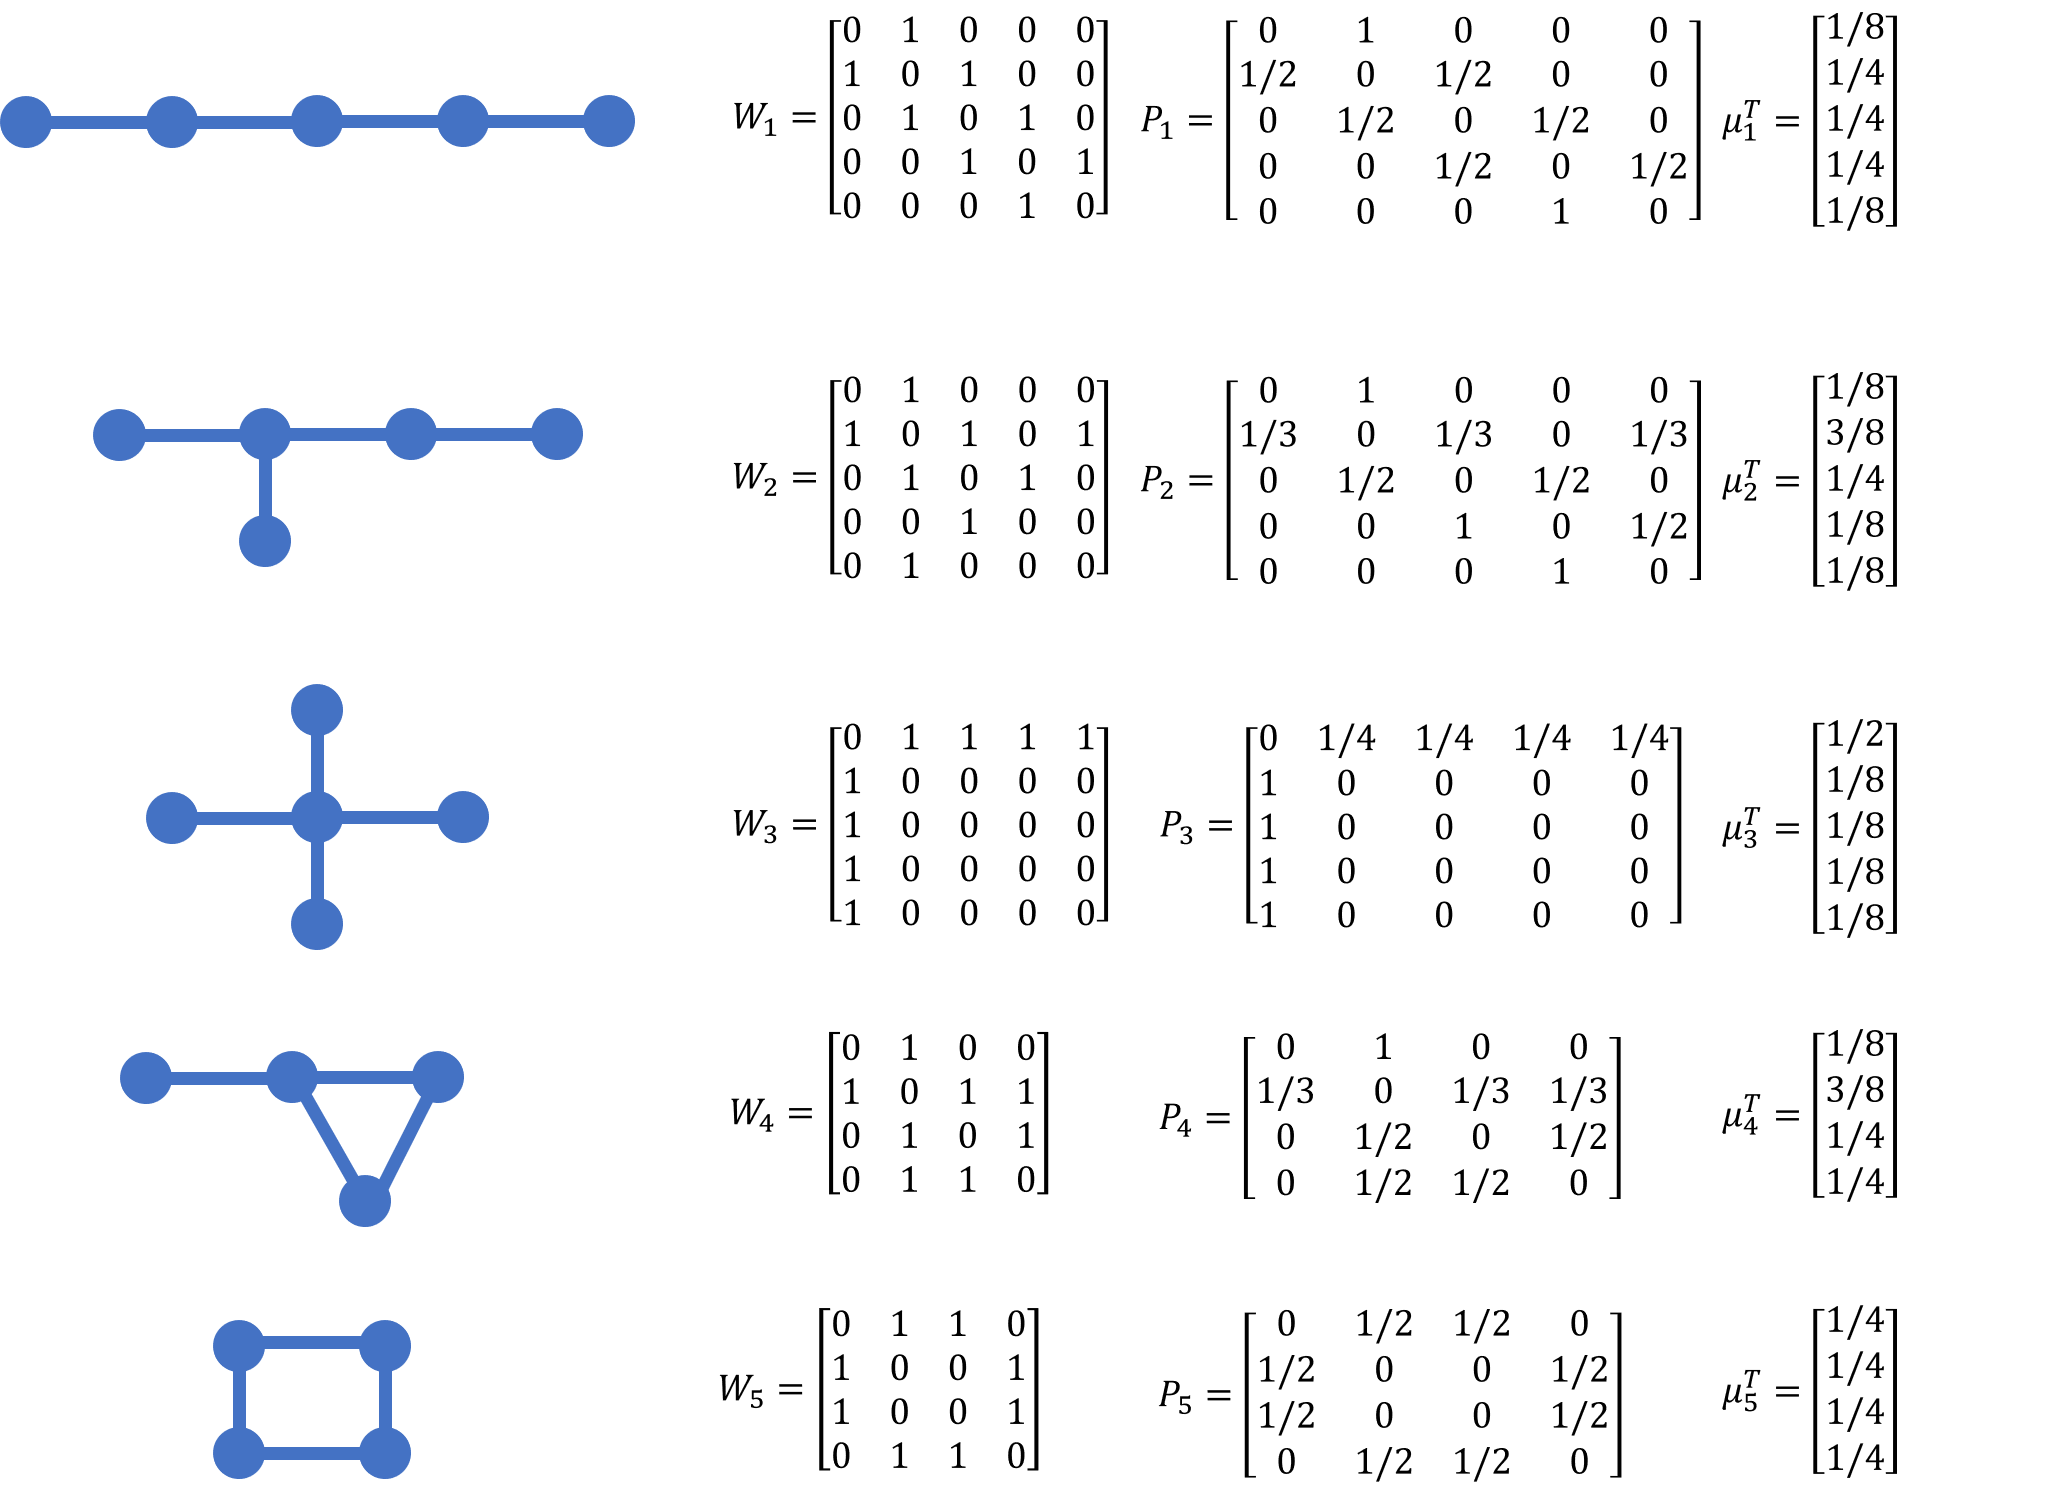
\includegraphics[width=16cm]{img/4-1.png}
        \caption{Five Possible Graphs for Four Edges}
        \label{fig:ex11}
      \end{figure}

      Their corresponding entropy rates are 0.75, 0.84436, 1, 1.09436 and 1.
  \begin{enumerate}
    \item {
    The fourth graph has the largest entropy rate.
    }
    \item { The first graph has the lowest entropy rate.
    }
  \end{enumerate}
  \end{solution}
  \label{ex11}
\end{exercise}

\section{Data Compression}
%%%%%%%%%%%%%%%%%%%%%%%%%%%%%%%%%%%%%%%%%%
%%%%%%%%%%%%%                 %%%%%%%%%%%%
%%%%%%%%%%%%%    EXERCISE 1   %%%%%%%%%%%%
%%%%%%%%%%%%%                 %%%%%%%%%%%%
%%%%%%%%%%%%%%%%%%%%%%%%%%%%%%%%%%%%%%%%%%
\begin{exercise}[Slackness in the Kraft inequality]{An instantaneous code has word lengths $l_{1}, l_{2}, \ldots, l_{m},$ which satisfy the strict inequality
  $\sum_{i=1}^{m} D^{-l_{i}}<1$
  The code alphabet is $\mathcal{D}=\{0,1,2, \ldots, D-1\} .$ Show that there exist arbitrarily long sequences of code symbols in $D^{*}$ which cannot be decoded into sequences of codewords.}
  \begin{proof}
  W.l.o.g., we assume $l_1\le l_2 \le \ldots \le l_m$. Since the coding method is instantaneous, for any coding with the length of $l_i$, there exists no other coding that begins with the $l_i$ corresponding coding. That is to say, if there exists a coding with $l_i$ length, then $D^{l_m-l_i}$ codewords of the $D^{l_m}$ codewords will be decodable. Adding all these decodable words up we have
  \begin{equation}
    \sum_{i=1}^{m} D^{l_m-l_i} = D^{l_m} \sum_{i=1}^{m} D^{-l_i} < D^{l_m}
  \end{equation}
  ,which implies that there exists some prefix words in $D^{l_m}$ that are undecodable. Any arbitrary word that begins with such prefix will be unable to decode into sequence of codewords.
  \end{proof}
  \label{ex1}
\end{exercise}

%%%%%%%%%%%%%%%%%%%%%%%%%%%%%%%%%%%%%%%%%%
%%%%%%%%%%%%%                 %%%%%%%%%%%%
%%%%%%%%%%%%%    EXERCISE 2   %%%%%%%%%%%%
%%%%%%%%%%%%%                 %%%%%%%%%%%%
%%%%%%%%%%%%%%%%%%%%%%%%%%%%%%%%%%%%%%%%%%
\begin{exercise}[Fix-free codes]{ A code is a fix-free code if it is both a prefix code and a suffix code. Let $l_{1}, l_{2}, \ldots, l_{m}$ be $m$ positive integers. Prove that if
  $\sum_{k=1}^{m} 2^{-l_{k}} \leq \frac{1}{2}$
  then there exists a binary fix-free code with codeword length $l_{1}, l_{2}, \ldots, l_{m}$}
  \begin{proof}
  W.l.o.g., we assume $l_1\le l_2 \le \ldots \le l_m$. We prove by induction on $m$.
  
  When $m=1$, the conclusion is trivial.

  We assume that when $m=k-1$, for any increasingly ordered positive integers $l_1,l_2,\ldots,l_{k-1}$, if $\sum_{i=1}^{k-1} 2^{-l_i} \le \frac{1}{2}$, then there exists a binary fix-free code with codeword length $l_1,l_2,\ldots,l_{k-1}$.

  Now let $m=k$. For every particular codeword, in terms of prefix codes, it will occupy the space of $2^{l_m - l_i}$ in the tree, while in terms of suffix codes, it wll also occpy the space of $2^{l_m - l_i}$ in the $2^{l_m}$ nodes. These two sets may overlap, but they will surely be less than $2\times 2^{l_m - l_i}$. Hence for all codewords, we have
  \begin{equation}
    2 \sum_{i=1}^{k} 2^{l_m - l_i} \le 2^{l_m} 
  \end{equation}
  
  
  It follows that $\sum_{i=1}^{k} 2^{-l_i} \le \frac{1}{2}$. By removing $l_k$ we have $\sum_{i=1}^{k-1} 2^{-l_i} < \frac{1}{2}$. By the induction hypothesis, we know that for $l_1,\ldots,l_{k-1}$ lengths of codewords, they can form a set of fix-free codes. Furthermore, the strict less relation tells us that there still remains space for the codeword $l_k$. Hence, the conclusion follows.
  \end{proof}
  \label{ex2}
\end{exercise}

%%%%%%%%%%%%%%%%%%%%%%%%%%%%%%%%%%%%%%%%%%
%%%%%%%%%%%%%                 %%%%%%%%%%%%
%%%%%%%%%%%%%    EXERCISE 3   %%%%%%%%%%%%
%%%%%%%%%%%%%                 %%%%%%%%%%%%
%%%%%%%%%%%%%%%%%%%%%%%%%%%%%%%%%%%%%%%%%%
\begin{exercise}[$\frac{3}{4}$ fix-free codes]{ Prove that when
  $$\sum_{k=1}^{m} 2^{-l_{k}} \leq \frac{3}{4}$$  the conclusion above holds.}
  \begin{proof} The proof here is not complete. We try to solve the problem from two perspectives. The proof idea is based on this paper\footnote{R. Ahlswede and B. Balkenhol and L. Khachatrian. Some properties of Fix-Free Codes}.
    \paragraph{There exists no upper bounds greater than $\frac{3}{4}$.} For any $\frac{3}{4}+\epsilon>\frac{3}{4}$, we choose $k$ such that $2^{-k}<\epsilon$. We construct a list of codelengths with $1$ and $2^{k-2}+1$ $k$s. Then we have
    \begin{equation}
      \sum_{i=1}^{N} 2^{-l_i} = \frac{1}{2}+ 2^{-k} (2^{k-2}+1) = \frac{3}{4}+\epsilon
    \end{equation}

    Our choice of codeword lengths satisfies our assumption, however, with the first codeword with length of 1 as a prefix and suffix, there are at most $2^{k-2}$ words of length $k$, which implies that our choice is invalid, contradiction. 

    \paragraph{The conclusion with $\frac{3}{4}$ holds under some restrictions.} We suppose that for all code lengths, either $l_i = l_{i+1}$ or $2l_i \le l_{i+1}$. We prove that under this restriction the conclusion will hold.

    W.l.o.g., we assume that $l_1 \le l_2 \le \ldots \le l_m$. We prove by induction on $m$. The base case of $m=1$ is trivial.

    Assume that for any $n\le m-1$, with $\sum_{i=1}^{n} 2^{-l_i} \le \frac{3}{4}$ we can construct $n$ different codeword lengths. We prove that this holds for the case of $m$.
    
    Let $m'$ be the largest index $i$ with $l_i < l_{m'}$. By induction hypothesis we can construct a fix-free code $C'$ with the lengths $l_1, \ldots, l_{m'}$. Note for every particular word with length $l_i$, it will occupy at most $2\times 2^{l_{m}-l_i}$ nodes due to the prefix and suffix rule. However, with our restriction, $2^{l_m - 2l_i}$ nodes will be returned, since they will not actually be used as codewords. Therefore, at the $l_m$ level, at most $2 \sum_{i=1}^{m'} 2^{l_m-l_i}- \sum_{i=1}^{m'}2^{l_{m} - 2l_i}$ nodes will be occupied.\footnote{The paper gives a more detailed formula, but I can't fully understand how the last component formula is derived. Fortunately leaving the that component out will not affect the proof here. }

    To ensure that the remaining $l_{m'+1},\ldots,l_m$ can be added to the orginal code system we should have

    \begin{equation}
      2 \sum_{i=1}^{m'} 2^{l_m -l_i}- \sum_{i=1}^{m'}2^{l_m - 2l_i} \le 2^{l_m} - (m -m')
      \label{eqn1}
    \end{equation}

    Writing $K = m - m'$ and $\alpha = \sum_{i=1}^{m'} 2^{-l_i}$. (\ref{eqn1}) can be written as

    \begin{equation}
      2\alpha - \alpha^2 \le 1 - \frac{K}{2^{l_m}}
    \end{equation}

    With abbreviation $\beta = \sum_{i=1}^{m} 2^{-l_i} = \alpha + \frac{K}{2^{l_m}}$ and $\delta = \frac{K}{2^{l_m}}$ we get the equivalent inequality

    \begin{equation}
      \beta \le 1+\delta - \sqrt{\delta}
    \end{equation}

    Note $\delta \in (0,1)$, the right side has the minimal value of $\frac{3}{4}$ at $\delta = \frac{1}{4}$. Thus for any $ \sum_{i=1}^{m} 2^{-l_i} \le \frac{3}{4}$, the conclusion holds.

  \end{proof}
  \label{ex3}
\end{exercise}

%%%%%%%%%%%%%%%%%%%%%%%%%%%%%%%%%%%%%%%%%%
%%%%%%%%%%%%%                 %%%%%%%%%%%%
%%%%%%%%%%%%%    EXERCISE 4   %%%%%%%%%%%%
%%%%%%%%%%%%%                 %%%%%%%%%%%%
%%%%%%%%%%%%%%%%%%%%%%%%%%%%%%%%%%%%%%%%%%
\begin{exercise}[More Huffman codes]{Find the binary Huffman code for the source with probabilities $\left(\frac{1}{3}, \frac{1}{5}, \frac{1}{5}, \frac{2}{15}, \frac{2}{15}\right) .$ Argue that this code is also optimal for the source with probabilities $\left(\frac{1}{5}, \frac{1}{5}, \frac{1}{5}, \frac{1}{5}, \frac{1}{5}\right)$}
  \begin{solution}
    \begin{figure}[H]
      \caption{Huffman Code for $\left(\frac{1}{3}, \frac{1}{5}, \frac{1}{5}, \frac{2}{15}, \frac{2}{15}\right) .$}
      \centering
      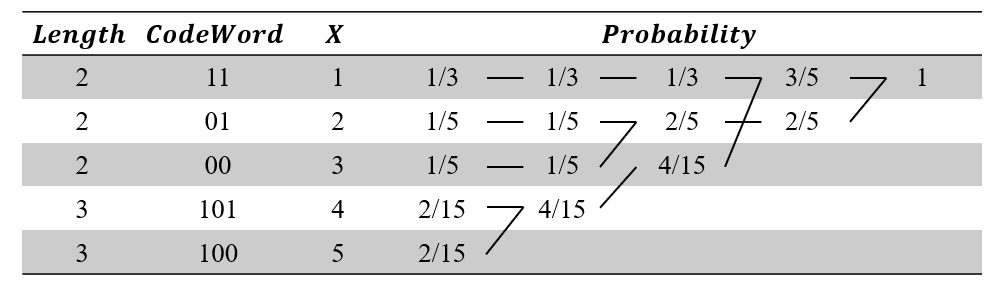
\includegraphics[width=11cm]{img/5-1.png}
      \label{fig:ex4}
    \end{figure}
    The huffman code of  $\left(\frac{1}{3}, \frac{1}{5}, \frac{1}{5}, \frac{2}{15}, \frac{2}{15}\right) .$ is found as Figure \ref{fig:ex4} shows. 

      \begin{figure}[H]
        \caption{Huffman Code for $\left(\frac{1}{5}, \frac{1}{5}, \frac{1}{5}, \frac{1}{5}, \frac{1}{5}\right)$}
        \centering
        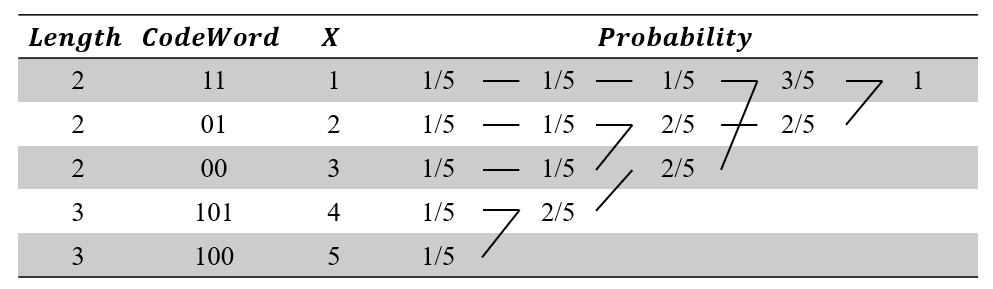
\includegraphics[width=11cm]{img/5-2.png}
        \label{fig:ex5}
      \end{figure}
    We see that for $\left(\frac{1}{5}, \frac{1}{5}, \frac{1}{5}, \frac{1}{5}, \frac{1}{5}\right)$, we can follow an identical process to construct the huffman code, as Figure \ref{fig:ex5} shows. Since huffman code is always optimal, the conclusion holds.
  \end{solution}
  \label{ex4}
\end{exercise}


%%%%%%%%%%%%%%%%%%%%%%%%%%%%%%%%%%%%%%%%%%
%%%%%%%%%%%%%                 %%%%%%%%%%%%
%%%%%%%%%%%%%    EXERCISE 5   %%%%%%%%%%%%
%%%%%%%%%%%%%                 %%%%%%%%%%%%
%%%%%%%%%%%%%%%%%%%%%%%%%%%%%%%%%%%%%%%%%%
\begin{exercise}[Bad codes]{ Which of these codes cannot be Huffman codes for any probability assignment?
  \begin{enumerate}
    \item \{0,10,11\}
    \item \{00,01,10,110\}
    \item \{01,10\}
  \end{enumerate}
  }
  \begin{solution}
  \par{~}
  \begin{enumerate}
    \item { \{0,10,11\} can be the huffman code for distribution $\left\{\frac{1}{2},\frac{1}{4},\frac{1}{4}\right\}$.
    }
    \item { \{00,01,10,110\} can be shortened by \{00,01,10,11\}. It cannot be a huffman code. 

    }
    \item { \{01,10\} can be shortened by \{0,1\}. It cannot be a huffman code.

    }
  \end{enumerate}
  \end{solution}
  \label{ex5}
\end{exercise}

%%%%%%%%%%%%%%%%%%%%%%%%%%%%%%%%%%%%%%%%%%
%%%%%%%%%%%%%                 %%%%%%%%%%%%
%%%%%%%%%%%%%    EXERCISE 6   %%%%%%%%%%%%
%%%%%%%%%%%%%                 %%%%%%%%%%%%
%%%%%%%%%%%%%%%%%%%%%%%%%%%%%%%%%%%%%%%%%%
\begin{exercise}[Huffman 20 questions]{ Consider a set of $n$ objects. Let $X_{i}=$ 1 or 0 accordingly as the $i$ th object is good or defective. Let $X_{1}, X_{2}, \ldots, X_{n}$ be independent with $\operatorname{Pr}\left\{X_{i}=1\right\}=p_{i} ;$ and $p_{1}>$
  $p_{2}>\cdots>p_{n}>\frac{1}{2} .$ We are asked to determine the set of all defective objects. Any yes-no question you can think of is admissible.
  \begin{enumerate}
    \item Give a good lower bound on the minimum average number of questions required. 
    \item If the longest sequence of questions is required by nature's answers to our questions, what (in words) is the last question we should ask? What two sets are we distinguishing with this question? Assume a compact (minimum average length) sequence of questions.
    \item Give an upper bound (within one question) on the minimum average number of questions required.
  \end{enumerate}}
  \begin{solution}
  \par{~}
  \begin{enumerate}
    \item { 
      The asking process can be modeled into the problem of constructing a compressed code for the sequence $X_1,X_2,\ldots,X_n$. The set of all defective objects can be determined if we determine the codeword we've constructed. The question we are asking is a yes-no question, so the codeword is based on a 2-ray alphabet. We can use entropy of $X_1,X_2,\ldots,X_n$ to give a lower bound on the average codeword length.
      \begin{equation}
        \begin{aligned}
          L^* &\ge H_2 (X_1,X_2,\ldots,X_n) \\
          &= \sum_{i=1}^{n} H(X_i) = \sum_{i=1}^{n} H(p_i)
        \end{aligned}
      \end{equation} 
    }
    \item { The longest sequence implies that we are distinguishing between the two least cases in this problem, i.e. the case where all objects are good ($\prod_{i=1}^n(1-p_i)$) and the case where all objects are good except the one that has the least probability to be defective ($p_n \prod_{i=1}^{n-1}(1-p_i)$). The question will be like ``Is $X_n$ defective?''.
    }
    \item { Using the same notion in part 1, the upper bound of the minimum average number of questions (codeword length) will be
    \begin{equation}
      \begin{aligned}
        L^* &\le H_2 (X_1,X_2,\ldots,X_n) + 1 \\
        &= \sum_{i=1}^{n} H(X_i) + 1 = \sum_{i=1}^{n} H(p_i) + 1
      \end{aligned}
    \end{equation}

    }
  \end{enumerate}
  \end{solution}
  \label{ex6}
\end{exercise}

%%%%%%%%%%%%%%%%%%%%%%%%%%%%%%%%%%%%%%%%%%
%%%%%%%%%%%%%                 %%%%%%%%%%%%
%%%%%%%%%%%%%    EXERCISE 7   %%%%%%%%%%%%
%%%%%%%%%%%%%                 %%%%%%%%%%%%
%%%%%%%%%%%%%%%%%%%%%%%%%%%%%%%%%%%%%%%%%%
\begin{exercise}[Simple optimum compression of a Markov source]{Consider the three-state Markov process $U_{1}, U_{2}, \ldots$ having transition matrix

  \begin{table}[H]
    \begin{center}
      \begin{tabular}{c|ccc}
      \diagbox{$U_n$}{$U_{n-1}$} & $S_1$         & $S_2$         & $S_3$         \\ \hline
      $S_1$                                         & $\frac{1}{2}$ & $\frac{1}{4}$ & $\frac{1}{4}$ \\
      $S_2$                                         & $\frac{1}{4}$ & $\frac{1}{2}$ & $\frac{1}{4}$ \\
      $S_3$                                         & 0             & $\frac{1}{2}$ & $\frac{1}{2}$
      \end{tabular}
    \end{center}
    \end{table}

  Thus, the probability that $S_{1}$ follows $S_{3}$ is equal to zero. Design three codes $C_{1}, C_{2}, C_{3}$ (one for each state 1,2 and $3,$ each code mapping elements of the set of $S_{i}$ 's into sequences of 0 's and 1 's, such that this Markov process can be sent with maximal compression by the following scheme: 
  \begin{enumerate}
    \item Note the present symbol $X_{n}=i$
    \item Select code $C_{i}$
    \item Note the next symbol $X_{n+1}=j$ and send the codeword in $C_{i}$ corresponding to $j$
    \item Repeat for the next symbol. 
  \end{enumerate}
  What is the average message length of the next symbol conditioned on the previous state $X_{n}=i$ using this coding scheme? What is the unconditional average number of bits per source symbol? Relate this to the entropy rate $H(\mathcal{U})$ of the Markov chain.
  }
  \begin{solution} We can design the codes using the Huffman method.
    \begin{table}[H]
      \begin{center}
        \begin{tabular}{c|ccc}
          & $S_1$         & $S_2$         & $S_3$         \\ \hline
        $C_1$                                         & 1 & 01 & 00 \\
        $C_2$                                         & 01 & 1 & 00 \\
        $C_3$                                         & N/A             & 0 & 1
        \end{tabular}
      \end{center}
    \end{table}
    We first calculate the stationery distribution of the Markov Chain.
    \begin{equation}
      \left\{\begin{array}{c}
        \mathbf{\mu}P = \mathbf{\mu} \\
        \mathbf{\mu} \mathbf{1}^T = 1
      \end{array}\right. \Rightarrow \mu = \left[\frac{2}{9}, \frac{4}{9},\frac{1}{3}\right]
    \end{equation}
    The average length is
    \begin{equation}
      \sum_{i=1}^{3} \mu_{i} \sum_{j=1}^{3} L(C_{ij}) = \frac{2}{9}\cdot\frac{3}{2} + \frac{4}{9} \cdot\frac{3}{2}+\frac{1}{3}\cdot 1 = \frac{4}{3}
    \end{equation}
    The entropy rate can be calculated as
    \begin{equation}
      H(\mathcal{U})=-\sum_{i j} \mu_{i} P_{i j} \log P_{i j} = \frac{4}{3}
    \end{equation}
    They are the same because the optimal code length is its entropy, which can be expressed with the notion of ``average'' entropy $\frac{1}{n} H(U_1,U_2,\ldots,U_n,\ldots)$, which approximates to $H(\mathcal{U})$.
  \end{solution}
  \label{ex7}
\end{exercise}

%%%%%%%%%%%%%%%%%%%%%%%%%%%%%%%%%%%%%%%%%%
%%%%%%%%%%%%%                 %%%%%%%%%%%%
%%%%%%%%%%%%%    EXERCISE 8   %%%%%%%%%%%%
%%%%%%%%%%%%%                 %%%%%%%%%%%%
%%%%%%%%%%%%%%%%%%%%%%%%%%%%%%%%%%%%%%%%%%
\begin{exercise}[Shannon codes and Huffman codes]{ Consider a random variable $X$ that takes on four values with probabilities $\left(\frac{1}{3}, \frac{1}{3}, \frac{1}{4}, \frac{1}{12}\right)$
  \begin{enumerate}
    \item Construct a Huffman code for this random variable.
    \item Show that there exist two different sets of optimal lengths for the codewords; namely, show that codeword length assignments (1,2,3,3) and (2,2,2,2) are both optimal.
    \item Conclude that there are optimal codes with codeword lengths for some symbols that exceed the Shannon code length $\left\lceil\log \frac{1}{p(x)}\right\rceil$
  \end{enumerate}
}
  \begin{solution}
  \par{~}
  \begin{enumerate}
    \item { A Huffman code is constructed as Figure \ref{fig:ex8-1} shows.
      \begin{figure}[H]
        \caption{Huffman Code for $\left(\frac{1}{3}, \frac{1}{3}, \frac{1}{4}, \frac{1}{12}\right)$}
        \centering
        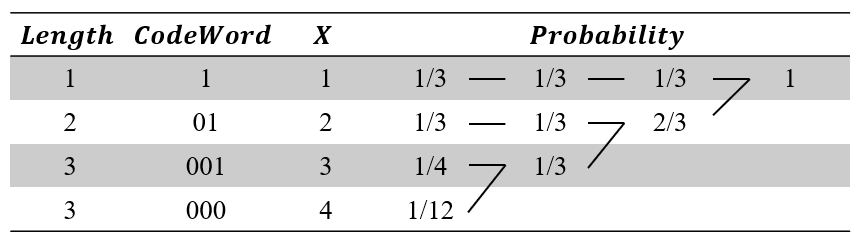
\includegraphics[width=11cm]{img/5-3.png}
        \label{fig:ex8-1}
      \end{figure}
    }
    \item { Another Huffman code is constructed as Figure \ref{fig:ex8-2} shows. They are both optimal for the distribution but with distinct length assignments.
      \begin{figure}[H]
        \caption{Huffman Code for $\left(\frac{1}{3}, \frac{1}{3}, \frac{1}{4}, \frac{1}{12}\right)$}
        \centering
        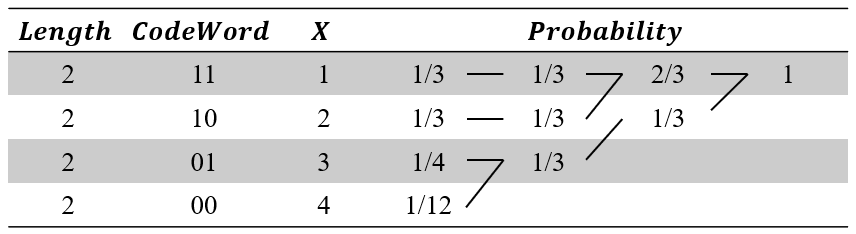
\includegraphics[width=11cm]{img/5-4.png}
        \label{fig:ex8-2}
      \end{figure}
    }
    \item { The case of $X=3$ in Figure \ref{fig:ex8-1} serves as an example. It has the length of 3, exceeding the Shannon length  $\left\lceil\log \frac{1}{p(x)}\right\rceil = 2$. It can be concluded that in some cases, we can construct optimal codes with codeword lengths for some symbols that exceed the Shannon code length.
    }
  \end{enumerate}
  \end{solution}
  \label{ex8}
\end{exercise}

%%%%%%%%%%%%%%%%%%%%%%%%%%%%%%%%%%%%%%%%%%
%%%%%%%%%%%%%                 %%%%%%%%%%%%
%%%%%%%%%%%%%    EXERCISE 9   %%%%%%%%%%%%
%%%%%%%%%%%%%                 %%%%%%%%%%%%
%%%%%%%%%%%%%%%%%%%%%%%%%%%%%%%%%%%%%%%%%%
\begin{exercise}[Data compression]{ Find an optimal set of binary codeword lengths $\left.l_{1}, l_{2}, \ldots \text { (minimizing } \sum p_{i} l_{i}\right)$ for an instantaneous code for each of the following probability mass functions:
  \begin{enumerate}
    \item $\mathbf{p}=\left(\frac{10}{41}, \frac{9}{41}, \frac{8}{41}, \frac{7}{41}, \frac{7}{41}\right)$
    \item $\mathbf{p}=\left(\frac{9}{10},\left(\frac{9}{10}\right)\left(\frac{1}{10}\right),\left(\frac{9}{10}\right)\left(\frac{1}{10}\right)^{2},\left(\frac{9}{10}\right)\left(\frac{1}{10}\right)^{3}, \ldots\right)$
  \end{enumerate}
  }
  \begin{solution} The optimal code is given in Figure \ref{fig:ex9} by the Huffman rule. Note that in problem (2) we have that any probability is greater than the sum of the probabilities less than itself. Hence, we can construct the Huffman code in a monotonous order
  \end{solution}
  \label{ex9}
\end{exercise}

\begin{figure}[htbp]
  \centering
  \caption{Huffman Code for Exercise \ref{ex9}}
      \begin{minipage}[t]{0.95\linewidth}
          \centering
          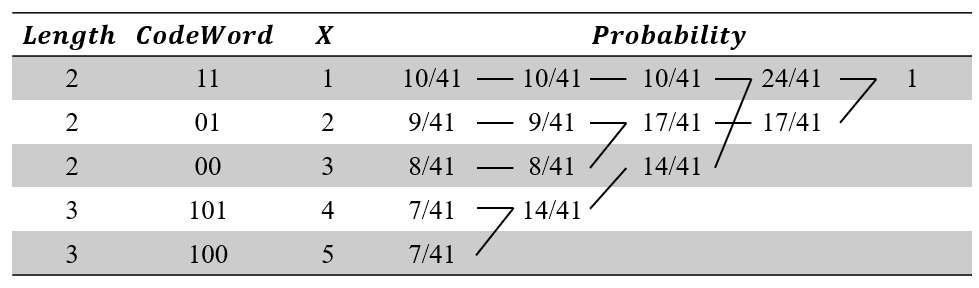
\includegraphics[width=11cm]{img/5-5.png}
      \end{minipage}
      \par{~}
      \begin{minipage}[t]{0.95\linewidth}
          \centering
          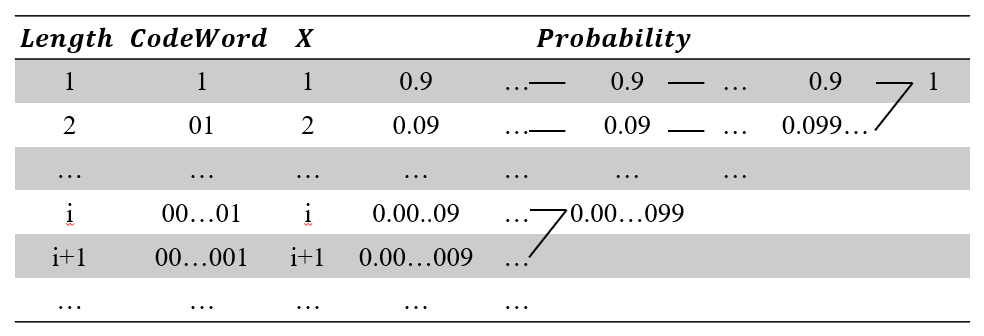
\includegraphics[width=11cm]{img/5-6.png}
      \end{minipage}
    \label{fig:ex9}
\end{figure}



\section{Information Channel}
%%%%%%%%%%%%%%%%%%%%%%%%%%%%%%%%%%%%%%%%%%
%%%%%%%%%%%%%                 %%%%%%%%%%%%
%%%%%%%%%%%%%    EXERCISE 1   %%%%%%%%%%%%
%%%%%%%%%%%%%                 %%%%%%%%%%%%
%%%%%%%%%%%%%%%%%%%%%%%%%%%%%%%%%%%%%%%%%%
\begin{exercise}[BSC]{Calculate the channel capacity of BSC.
  \begin{figure}[H]
    \centering
    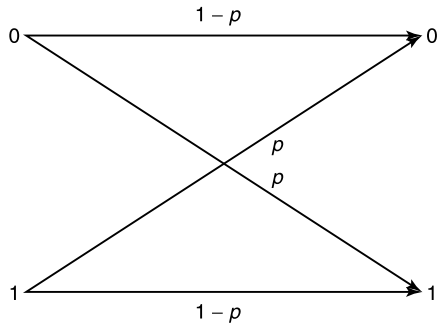
\includegraphics[height=3cm]{img/6-1.png}
    \caption{Binary Symmetric Channel}
    \label{fig:bsc}
  \end{figure}}
  \begin{solution}
  \begin{equation}\begin{aligned}
    C &=\max_{p(x)} I(X ; Y) \\
    &=\max_{p(x)} (H(Y)-H(Y | X) )\\
    &=\max_{p(x)} (H(Y)-\sum p(x) H(Y | X=x) )\\
    &=\max_{p(x)} (H(Y)-\sum p(x) H(p)) \\
    &=\max_{p(x)} (H(Y) - H(p)) = \log 2 - H(p)
    \end{aligned}\end{equation}
  The maximal value can be obtained when $X$ and $Y$ are uniformly distributed.
  \end{solution}
  \label{ex1}
\end{exercise}

%%%%%%%%%%%%%%%%%%%%%%%%%%%%%%%%%%%%%%%%%%
%%%%%%%%%%%%%                 %%%%%%%%%%%%
%%%%%%%%%%%%%    EXERCISE 2   %%%%%%%%%%%%
%%%%%%%%%%%%%                 %%%%%%%%%%%%
%%%%%%%%%%%%%%%%%%%%%%%%%%%%%%%%%%%%%%%%%%
\begin{exercise}[BSC]{Calculate the channel capacity of BEC.
  \begin{figure}[H]
    \centering
    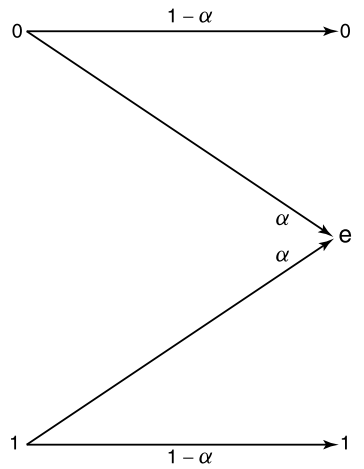
\includegraphics[height=4cm]{img/6-2.png}
    \caption{Binary Erasure Channel}
    \label{fig:bec}
  \end{figure}}
  \begin{solution}
    \begin{equation}\begin{aligned}
      C &=\max _{p(x)} I(X ; Y) \\
      &=\max _{p(x)}(H(Y)-H(Y | X))\\
      &=\max _{p(x)} (H(Y)-H(\alpha))
      \end{aligned}\end{equation}
      Let $\Pr\left(X = 1\right) = \pi$, then
      \begin{equation}
        \begin{aligned}
          H(Y) &= H((1-\pi)(1-\alpha),\alpha,\pi(1-\alpha)) \\
          &= H(\alpha) + (1-\alpha)H(\pi) \\
          C &= \max_{p(x)} (H(Y)-H(\alpha)) \\
          &= \max_{\pi} ((1-\alpha)H(\pi)+H(\alpha)-H(\alpha)) \\
          &= \max_{\pi} (1-\alpha)H(\pi) = 1-\alpha
        \end{aligned}
      \end{equation}
      The maximal value can be obtained when $X$ is uniformly distributed.
  \end{solution}
  \label{ex2}
\end{exercise}

%%%%%%%%%%%%%%%%%%%%%%%%%%%%%%%%%%%%%%%%%%
%%%%%%%%%%%%%                 %%%%%%%%%%%%
%%%%%%%%%%%%%    EXERCISE 3   %%%%%%%%%%%%
%%%%%%%%%%%%%                 %%%%%%%%%%%%
%%%%%%%%%%%%%%%%%%%%%%%%%%%%%%%%%%%%%%%%%%
\begin{exercise}[Using two channels at once]{Consider two discrete memoryless channels $\left(\mathcal{X}_{1}, p\left(y_{1} | x_{1}\right), \mathcal{Y}_{1}\right)$ and $\left(\mathcal{X}_{2}, \right.$  $\left. p\left(y_{2} | x_{2}\right), \mathcal{Y}_{2}\right)$ with capacities $C_{1}$ and $C_{2}$ respectively. A new channel $\left(\mathcal{X}_{1} \times \mathcal{X}_{2}, p\left(y_{1} | x_{1}\right) \times p\left(y_{2} | x_{2}\right), \mathcal{Y}_{1} \times \mathcal{Y}_{2}\right)$ is formed in which $x_{1} \in \mathcal{X}_{1}$ and $x_{2} \in \mathcal{X}_{2}$ are sent simultaneously, resulting in $\mathcal{Y}_{1}, \mathcal{Y}_{2} .$ Find the capacity of this channel.}
  \begin{solution} By condition we know that $p(y_1,y_2|x_1,x_2) = p\left(y_{1} | x_{1}\right) \times p\left(y_{2} | x_{2}\right)$. It follows by definition that 
    \begin{equation}
      H(Y_1,Y_2|X_1,X_2) = H(Y_1|X_1)+H(Y_2|X_2).
    \end{equation}
    Therefore, 
    \begin{equation}
      \begin{aligned}
        I(X_1,X_2;Y_1,Y_2) &= H(Y_1,Y_2) - H(Y_1,Y_2|X_1,X_2) \\
        &= H(Y_1,Y_2) - H(Y_1|X_1) - H(Y_2|X_2) \\
        &\le H(Y_1) + H(Y_2) - H(Y_1|X_1) - H(Y_2|X_2) \\
        &= I(Y_1;X_1) + I(Y_2;X_2) \\
        &\le C_1 + C_2
      \end{aligned}
    \end{equation}
    Hence $C = C_1 +C_2$. The equality holds when $p(x_1,x_2) = p^{*}(x_1) p^{*}(x_2)$, where $p^{*}(x_1)$ and $p^{*}(x_2)$ are the optimal distribution corresponding to the original channel capacities.
  \end{solution}
  \label{ex3}
\end{exercise}

%%%%%%%%%%%%%%%%%%%%%%%%%%%%%%%%%%%%%%%%%%
%%%%%%%%%%%%%                 %%%%%%%%%%%%
%%%%%%%%%%%%%    EXERCISE 4   %%%%%%%%%%%%
%%%%%%%%%%%%%                 %%%%%%%%%%%%
%%%%%%%%%%%%%%%%%%%%%%%%%%%%%%%%%%%%%%%%%%
\begin{exercise}[Z-channel]{ The Z-channel has binary input and output alphabets and transition probabilities $p(y | x)$ given by the following matrix:
$$Q=\left[\begin{array}{ll}1 & 0 \\ \frac{1}{2} & \frac{1}{2}\end{array}\right], x, y \in\{0,1\}$$
Find the capacity of the Z-channel and the maximizing input probability distribution.
\begin{figure}[H]
  \centering
  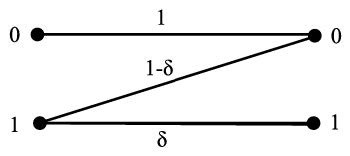
\includegraphics[height=2.5cm]{img/6-3.jpg}
  \caption{Z-Channel}
  \label{fig:z-chan}
\end{figure}
}
  \begin{solution}
  Assume that $\Pr(X=1)=\pi$, given the transition matrix $Q$, we have that $\Pr(Y=1) = \frac{\pi}{2}$, $\Pr(Y=1) = 1 - \frac{\pi}{2}$.
  \begin{equation}
    \begin{aligned}
      I(X;Y)&= H(Y) - H(Y|X) \\
      &= H(\frac{\pi}{2}) - \pi H(\frac{1}{2}) - (1-\pi)H(1) \\
      &= -\frac{\pi}{2} \log(\frac{\pi}{2}) - \left(1 - \frac{\pi}{2}\right) \log \left(1 - \frac{\pi}{2}\right) - \pi
    \end{aligned}
  \end{equation}
  Since the function is a concave function, we find its maximal value by taking the derivative.
  \begin{equation}
    \begin{aligned}
      \frac{dI(X;Y)}{d\pi} &= -\frac{1}{2} \log(\frac{\pi}{2}) - \frac{1}{2\ln 2} + \frac{1}{2\ln 2} + \left(1 - \frac{1}{2}\right) \log \left(1 - \frac{\pi}{2}\right) -1 \\
      &= \frac{1}{2} \log \frac{2-\pi}{\pi} - 1 := 0      
    \end{aligned}
  \end{equation}
  It follows that the mutual information is at its maximum when $\pi = \frac{2}{5}$. The channel capacity is $C \approx 0.32193$.
  \end{solution}
  \label{ex4}
\end{exercise}

%%%%%%%%%%%%%%%%%%%%%%%%%%%%%%%%%%%%%%%%%%
%%%%%%%%%%%%%                 %%%%%%%%%%%%
%%%%%%%%%%%%%    EXERCISE 5   %%%%%%%%%%%%
%%%%%%%%%%%%%                 %%%%%%%%%%%%
%%%%%%%%%%%%%%%%%%%%%%%%%%%%%%%%%%%%%%%%%%
\begin{exercise}[Erasures and errors in a binary channel]{Consider a channel with binary inputs that has both erasures and errors. Let the probability of error be $\epsilon$ and the probability of erasure be $\alpha,$ so the channel is follows:
  \begin{figure}[H]
    \centering
    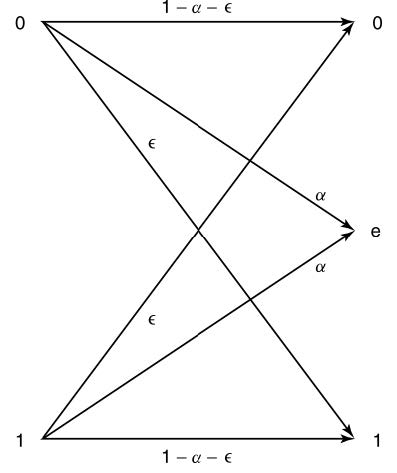
\includegraphics[height=5cm]{img/6-4.jpg}
    \caption{Erasures and Errors}
    \label{fig:err}
  \end{figure}
  Find the capacity of this channel.}
  \begin{solution}
    The transition matrix is as follows.
    \begin{table}[H]
      \begin{center}
        \begin{tabular}{c|ccc}
         \diagbox{X}{Y} & 0             & e             & 2             \\ \hline
        0 & $1-\alpha-\epsilon$ & $\alpha$ & $\epsilon$             \\
        1 & $\epsilon$            & $\alpha$ & $1-\alpha-\epsilon$
        \end{tabular}
      \end{center}
      \end{table}
      The matrix is row symmetric, we have that
      \begin{equation}
        I(X ; Y) = H(Y)-H(Y | X) = H(Y) - H(\alpha,\epsilon,1-\alpha-\epsilon)
      \end{equation}
      Furthermore, note that the distribution of $Y$ in terms of the distribution of $X$ is symmetric, i.e. 
      \begin{equation}
        H(Y) \arrowvert_{\Pr(X=0)=\pi} = H(Y) \arrowvert_{\Pr(X=0)=1 - \pi}
      \end{equation}
      and that the entropy function is a concave function. It follows that the maximal value must be obtained at $p(x) = \frac{1}{2}$ for $x = 0,1$.
      \begin{equation}
        C = H(\frac{1-\alpha}{2},\alpha,\frac{1-\alpha}{2}) - H(\alpha,\epsilon,1-\alpha-\epsilon)
      \end{equation}
  \end{solution}
  \label{ex5}
\end{exercise}

%%%%%%%%%%%%%%%%%%%%%%%%%%%%%%%%%%%%%%%%%%
%%%%%%%%%%%%%                 %%%%%%%%%%%%
%%%%%%%%%%%%%    EXERCISE 6   %%%%%%%%%%%%
%%%%%%%%%%%%%                 %%%%%%%%%%%%
%%%%%%%%%%%%%%%%%%%%%%%%%%%%%%%%%%%%%%%%%%
\begin{exercise}[Additive noise channel]{Find the channel capacity of the following discrete memoryless channel:
\begin{figure}[H]
  \centering
  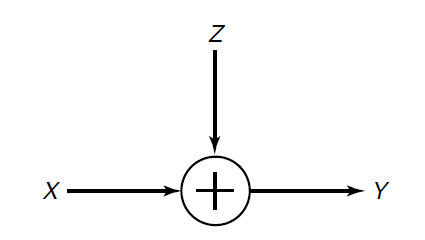
\includegraphics[height=3cm]{img/6-5.png}
  \caption{Discrete Memoryless Channel}
  \label{fig:ex6}
\end{figure}
where $\operatorname{Pr}\{Z=0\}=\operatorname{Pr}\{Z=a\}=\frac{1}{2} .$ The alphabet for $x$ is $\mathbf{X}=$ \{0,1\} . Assume that $Z$ is independent of $X .$ Observe that the channel capacity depends on the value of $a$. }
  \begin{solution}
  The condition implies that $a\neq 0$, but after the plus operation the distribution of $Y$ may vary. Hence we discuss the value of $a$ in several cases.
  \begin{enumerate}
    \item {
      $a = \pm 1$, the result of $X + a$ and $X + 0$ may overlap. We take the case of $a = 1$ as example. The transition matrix is as follows.
      \begin{table}[H]
        \begin{center}
          \begin{tabular}{c|ccc}
           \diagbox{X}{Y} & 0             & 1             & 2             \\[2mm] \hline
          0 & $\frac{1}{2}$ & $\frac{1}{2}$ & 0             \\[2mm]
          1 & 0             & $\frac{1}{2}$ & $\frac{1}{2}$
          \end{tabular}
        \end{center}
        \end{table}
        The matrix is row symmetric, assume that $\Pr(X = 0) = \pi$we have that
        \begin{equation}
          \begin{aligned}
          I(X ; Y) &=H(Y)-H(Y | X) \\
          &=H(\frac{1}{2}\pi,\frac{1}{2},\frac{1}{2}\pi)-H(\frac{1}{2}) \\
          & \leq H(\frac{1}{4},\frac{1}{4},\frac{1}{2}\pi)-H(\frac{1}{2}) = \frac{1}{2}
          \end{aligned}
        \end{equation}
        $C = \frac{1}{2}$. The maximal value is obtained at $\pi = \frac{1}{2}$.
    }
    \item{$a \neq \pm 1$. Then the output $Y$ will not overlap for different $X$. Hence $Y$ is a function of $X$. We have
    \begin{equation}
      C=\max I(X ; Y)=\max H(X) = 1
    \end{equation}
    The maximal value is obtained when $p(x) = \frac{1}{2}$ for $x=0,1$.
    }
  \end{enumerate}
  \end{solution}
  \label{ex6}
\end{exercise}

%%%%%%%%%%%%%%%%%%%%%%%%%%%%%%%%%%%%%%%%%%
%%%%%%%%%%%%%                 %%%%%%%%%%%%
%%%%%%%%%%%%%    EXERCISE 7   %%%%%%%%%%%%
%%%%%%%%%%%%%                 %%%%%%%%%%%%
%%%%%%%%%%%%%%%%%%%%%%%%%%%%%%%%%%%%%%%%%%
\begin{exercise}[Channel capacity]{Consider the discrete memoryless channel $Y=$ $X+Z(\bmod 11),$ where
  $$
  Z=\left(\begin{array}{ccc}
  1, & 2, & 3 \\
  \frac{1}{3}, & \frac{1}{3}, & \frac{1}{3}
  \end{array}\right)
  $$
  and $X \in\{0,1, \ldots, 10\} .$ Assume that $Z$ is independent of $X$.
  \begin{enumerate}
    \item Find the capacity.
    \item What is the maximizing $p^{*}(x) ?$
  \end{enumerate}}
  \begin{solution} Note that the transition matrix of this channel is
    \begin{table}[H]
      \begin{center}
        \begin{tabular}{c|cccccc}
          \diagbox{$X$}{$Y$}         & 0             & 1             & 2             & $\ldots$ & 9        & 10            \\[2mm] \hline
        0        & 0             & $\frac{1}{3}$ & $\frac{1}{3}$ & $\ldots$ & 0        & 0             \\[2mm]
        1        & 0             & 0             & $\frac{1}{3}$ & $\ldots$ & 0        & 0             \\[2mm]
        2        & 0             & 0             & 0             & $\ldots$ & 0        & 0             \\[2mm]
        $\vdots$ & $\vdots$      & $\vdots$      & $\vdots$      & $\ddots$ & $\vdots$ & $\vdots$      \\[2mm]
        9        & $\frac{1}{3}$ & $\frac{1}{3}$ & 0             & $\ldots$ & 0        & $\frac{1}{3}$ \\[2mm]
        10       & $\frac{1}{3}$ & $\frac{1}{3}$ & $\frac{1}{3}$ & $\ldots$ & 0        & 0            
        \end{tabular}
      \end{center}
    \end{table}
    Note that the matrix is both column and row symmetric. Therefore we have
    \begin{equation}
      \begin{aligned}
        I(X ; Y) &=H(Y)-H(Y | X) \\
        &=H(Y)-H(\mathbf{r}) \\
        & \leq \log |\mathcal{Y}|-H(\mathbf{r}) = \log 11 - \log 3 = \log \frac{11}{3}
        \end{aligned}
    \end{equation}
    $C = \log \frac{11}{3}$. The maximal value is obtained when $p^{*}(x) = \frac{1}{11}$ for every $x \in \{0,1, \ldots, 10\}$
  \end{solution}
  \label{ex7}
\end{exercise}

%%%%%%%%%%%%%%%%%%%%%%%%%%%%%%%%%%%%%%%%%%
%%%%%%%%%%%%%                 %%%%%%%%%%%%
%%%%%%%%%%%%%    EXERCISE 8   %%%%%%%%%%%%
%%%%%%%%%%%%%                 %%%%%%%%%%%%
%%%%%%%%%%%%%%%%%%%%%%%%%%%%%%%%%%%%%%%%%%
\begin{exercise}[Zero-error capacity]{A channel with alphabet \{0,1,2,3,4\} has transition probabilities of the form
  $$
  p(y | x)=\left\{\begin{array}{cl}
  1 / 2 & \text { if } y=x \pm 1 \bmod 5 \\
  0 & \text { otherwise }
  \end{array}\right.
  $$
  (a) Compute the capacity of this channel in bits.

  (b) The zero-error capacity of a channel is the number of bits per channel use that can be transmitted with zero probability of error. Clearly, the zero-error capacity of this pentagonal channel is at least 1 bit (transmit 0 or 1 with probability $1 / 2$ ). Find a block code that shows that the zero-error capacity is greater than 1 bit. Can you estimate the exact value of the zero-error capacity? (Hint: Consider codes of length 2 for this channel.)}
  \begin{solution}
  \begin{enumerate}
    \item {
      Note that the transition matrix is row and column symmetric. It follows that
      \begin{equation}
        \begin{aligned}
          I(X ; Y) &=H(Y)-H(Y | X) \\
          &=H(Y)-H(\frac{1}{2}) \\
          & \leq \log |\mathcal{Y}|-H(\frac{1}{2}) = \log 5 - 1 \approx1.322
          \end{aligned}
      \end{equation}
      $C = 1.322$ bits. The maximal value is obtained when $X$ and $Y$ are uniformly distributed.
    }
    \item {
      According to the hint, we try to build a 2-tuple code with the alphabet \{0,1,2,3,4\}. Note that for every input codeword $\left(X_1,X_2\right)$, there are four possibilities of output, namely $\left((X_1 \pm 1) \bmod 5 ,(X_1 \pm 1) \bmod 5\right)$, but the good news is that if we can ensure that there are no other input codewords (and their possible outputs) occupying the 4 entries, we can infer the input determintly.
      
      Figure \ref{fig:ex8} gives an example of zero-error codes, where cells identified by different colors represent a codeword. The input codewords are (0,0),(1,2),(2,4),(3,1) and (4,3). Given an output codeword, its corresponding input codeword can be determined directly from the table.
      \begin{figure}[H]
        \centering
        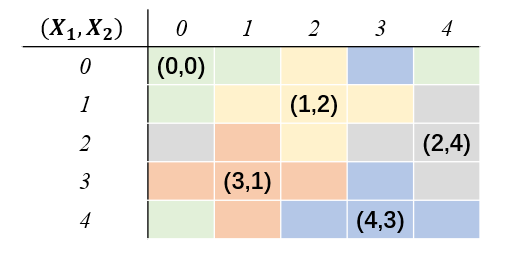
\includegraphics[]{img/6-6.png}
        \caption{A Construction of Zero-Error Codes}
        \label{fig:ex8}
      \end{figure}

      With the codes above, we can find that the number of bits per channel use is $\frac{1}{2} \log{5} > 1$.
    }
  \end{enumerate}
  \end{solution}
  \label{ex8}
\end{exercise}

\section{Channel Capacity}
%%%%%%%%%%%%%%%%%%%%%%%%%%%%%%%%%%%%%%%%%%
%%%%%%%%%%%%%                 %%%%%%%%%%%%
%%%%%%%%%%%%%    EXERCISE 1   %%%%%%%%%%%%
%%%%%%%%%%%%%                 %%%%%%%%%%%%
%%%%%%%%%%%%%%%%%%%%%%%%%%%%%%%%%%%%%%%%%%
\begin{exercise}[Capacity of the carrier pigeon channel]{Consider a commander of an army besieged in a fort for whom the only means of communication to his allies is a set of carrier pigeons. Assume that each carrier pigeon can carry one letter (8 bits), that pigeons are released once every 5 minutes, and that each pigeon takes exactly 3 minutes to reach its destination.
  \begin{enumerate}
    \item Assuming that all the pigeons reach safely, what is the capacity of this link in bits/hour?
    \item Now assume that the enemies try to shoot down the pigeons and that they manage to hit a fraction $\alpha$ of them. since the pigeons are sent at a constant rate, the receiver knows when the pigeons are missing. What is the capacity of this link?
    \item Now assume that the enemy is more cunning and that every time they shoot down a pigeon, they send out a dummy pigeon carrying a random letter (chosen uniformly from all 8-bit letters). What is the capacity of this link in bits/hour? Set up an appropriate model for the channel in each of the above cases, and indicate how to go about finding the capacity.
  \end{enumerate}}
  \begin{solution}
  \par{~}
  \begin{enumerate}
    \item { The capacity is 8 bits/5mins $=$ 96 bits/hour.
    }
    \item { The process can be modeled as an erasure model. Consider the transmission of a pigeon of 8 bits (256 alphabets), it has the probability of $\alpha$ to be erased. We assume the message sent is $X \in \left\{0, \ldots, 256 \right\}$, the message received is $Y \in \left\{e, 0, \ldots, 256\right\}$. The capacity of a single transmission is
    \begin{equation}
      \begin{aligned}
        C &=\max _{p(x)} I(X ; Y) \\
        &=\max _{p(x)}(H(Y)-H(Y | X))\\
        &=\max _{p(x)} (H(Y)-H(\alpha)) \\
        &=\max _{\pi}((1-\alpha) H(Y|X = Y)+H(\alpha)-H(\alpha))\\
        &=\log(256) (1- \alpha)
      \end{aligned}
    \end{equation}  
    Hence the capacity is $8(1-\alpha)$ bits per pigeon, or $96(1-\alpha)$ bits per hour.
    }
    \item { The process can be modeled as a binary symmetric channel. Consider the transmission of a pigeon of 8 bits (256 alphabets), it has the probability of $\frac{\alpha}{256}$ to be changed to a different value. We assume the message sent is $X \in \left\{0, \ldots, 256 \right\}$, the message received is $Y \in \left\{0, \ldots, 256\right\}$. The capacity of a single transmission is
    \begin{equation}
      \begin{aligned}
        C&=\max I(X ; Y) \\
 &=\max H(Y)-H(Y | X) \\
 &=\max H(Y)-\sum p(x) H(Y | X=x) \\
 &=\max H(Y)-H\left(1 - \frac{255\alpha}{256}, \frac{\alpha}{256}, \ldots, \frac{\alpha}{256}\right) \\
 &= 16 + \frac{255}{256}\alpha \log \frac{256-255\alpha}{\alpha} - \log (256 - 255\alpha) 
        \end{aligned}
    \end{equation}  
    Hence the capacity is $16 + \frac{255}{256}\alpha \log \frac{256-255\alpha}{\alpha} - \log (256 - 255\alpha)$ bits per pigeon, or $12(16 + \frac{255}{256}\alpha \log \frac{256-255\alpha}{\alpha} - \log (256 - 255\alpha))$ bits per hour.
    
    }
  \end{enumerate}
  \end{solution}
  \label{ex7-1}
\end{exercise}

%%%%%%%%%%%%%%%%%%%%%%%%%%%%%%%%%%%%%%%%%%
%%%%%%%%%%%%%                 %%%%%%%%%%%%
%%%%%%%%%%%%%    EXERCISE 2   %%%%%%%%%%%%
%%%%%%%%%%%%%                 %%%%%%%%%%%%
%%%%%%%%%%%%%%%%%%%%%%%%%%%%%%%%%%%%%%%%%%
\begin{exercise}[Channel with two independent looks at $Y$]{ Let $Y_{1}$ and $Y_{2}$ be conditionally independent and conditionally identically distributed given
  $X$
  \begin{enumerate}
    \item Show that $I\left(X ; Y_{1}, Y_{2}\right)=2 I\left(X ; Y_{1}\right)-I\left(Y_{1}, Y_{2}\right)$
    \item Conclude that the capacity of the channel $(X\mapsto Y_1,Y_2)$ is less than twice the capacity of channel $(X \mapsto Y_1)$
  \end{enumerate} }
  \begin{proof}
  \par{~}
  \begin{enumerate}
    \item {
      \begin{equation}
        \begin{aligned}
          I(X;Y_1,Y_2) &= H(Y_1,Y_2) - H(Y_1,Y_2|X) \\
          &= H(Y_1,Y_2) - H(Y_1|X) - H(Y_2|X) \\
          &= H(Y_1) + H(Y_2) - I(Y_1;Y_2) -  H(Y_1|X) - H(Y_2|X) \\
          &=I(X;Y_1) + I(X;Y_2)- I(Y_1,Y_2) \\
          &= 2I(X;Y_1) - I(Y_1,Y_2)
        \end{aligned}
      \end{equation}
     }
    \item { 
\begin{equation}
  \begin{aligned}
    C_1 &= \max_{p(x)} I(X;Y_1,Y_2) \\
    &= \max_{p(x)} (2I(X;Y_1) - I(Y_1,Y_2)) \\
    &\le \max_{p(x)} 2I(X;Y_1) \\
    &= 2C_2
  \end{aligned}
\end{equation}
    }
  \end{enumerate}
  \end{proof}
  \label{ex7-2}
\end{exercise}

%%%%%%%%%%%%%%%%%%%%%%%%%%%%%%%%%%%%%%%%%%
%%%%%%%%%%%%%                 %%%%%%%%%%%%
%%%%%%%%%%%%%    EXERCISE 3   %%%%%%%%%%%%
%%%%%%%%%%%%%                 %%%%%%%%%%%%
%%%%%%%%%%%%%%%%%%%%%%%%%%%%%%%%%%%%%%%%%%
\begin{exercise}[Binary multiplier channel]{\par{~}
  \begin{enumerate}
    \item Consider the channel $Y=X Z$, where $X$ and $Z$ are independent binary random variables that take on values 0 and $1 . Z$ is Bernoulli($\alpha \text {) [i.e., } P(Z=1)=\alpha] .$ Find the capacity of this channel and the maximizing distribution on $X$.
    \item Now suppose that the receiver can observe $Z$ as well as $Y$. What is the capacity?
  \end{enumerate} }
  \begin{solution}
  \par{~}
  \begin{enumerate}
    \item { Let $p(X=1)= \pi$
    \begin{equation}
      \begin{aligned}
        I(Y;X) &= H(Y) - H(Y|X) \\
        &= H(\alpha \pi) - \pi H(\alpha) \\
        &= - \alpha\pi \log \alpha\pi - (1 - \alpha\pi) \log (1- \alpha\pi) - H(\alpha)\pi
       \end{aligned}
    \end{equation}
    We find the maximal value by taking the derivative.
    \begin{equation}
      \begin{aligned}
        \frac{dI(Y;X)}{d\pi} &= - \alpha \log \alpha\pi - \frac{\alpha}{\ln 2} + \alpha \log (1-\alpha \pi) + \frac{\alpha}{\ln 2} - H(\alpha) \\
        &= \alpha \log \frac{1-\alpha\pi}{\alpha\pi} - H(\alpha) := 0 \\
        \frac{1-\alpha\pi}{\alpha\pi} &= 2^{\frac{H(\alpha)}{\alpha}} \\
        \pi^{*} &= \frac{1}{\alpha\left(2^{\frac{H(\alpha)}{\alpha}}+1\right)} \\
        C &= \log \left(2^{\frac{H(\alpha)}{\alpha}}+1\right)-\frac{H(\alpha)}{\alpha}
      \end{aligned}
    \end{equation}
    }
    \item { Let $p(X=1)= \pi$
    \begin{equation}
      \begin{aligned}
        I(Y,Z;X) &= H(Y,Z) - H(Y,Z|X) \\
        &= H(Y|Z) + H(Z) - H(Y|Z,X) - H(Z|X) \\
        &= H(Y|Z) - H(XZ|Z,X) = H(XZ|Z) \\
        &= \alpha H(\pi) \le \alpha
       \end{aligned}
    \end{equation}
    The maximal value is obtained when $X$ is normally distributed.
    }
  \end{enumerate}
  \end{solution}
  \label{ex7-3}
\end{exercise}

%%%%%%%%%%%%%%%%%%%%%%%%%%%%%%%%%%%%%%%%%%
%%%%%%%%%%%%%                 %%%%%%%%%%%%
%%%%%%%%%%%%%    EXERCISE 4   %%%%%%%%%%%%
%%%%%%%%%%%%%                 %%%%%%%%%%%%
%%%%%%%%%%%%%%%%%%%%%%%%%%%%%%%%%%%%%%%%%%
\begin{exercise}[Noise Channel]{Consider the channel $\mathcal{X}=\{0,1,2,3\},$ where $Y=X+Z,$ and $Z$ is uniformly distributed over three distinct integer values $\mathcal{Z}=\left\{z_{1}, z_{2}, z_{3}\right\}$
  \begin{enumerate}
    \item What is the maximum capacity over all choices of the $\mathcal{Z}$ alphabet? Give distinct integer values $z_{1}, z_{2}, z_{3}$ and a distribution on     $\mathcal{X}$ achieving this.
    \item What is the minimum capacity over all choices for the $\mathcal{Z}$ alphabet? Give distinct integer values $z_{1}, z_{2}, z_{3}$ and a distribution on
    $\mathcal{X}$ achieving this.
  \end{enumerate} }
  \begin{solution}
  \par{~}
  \begin{enumerate}
    \item { 
    \begin{equation}
      \begin{aligned}
        I(Y;X) &= H(X) - H(X|X+Z) \\
        &\le H(x)  \le \log 4 = 2
      \end{aligned}
    \end{equation}  
    The maximal capacity will be achieved when $X$ is a function of $Y$, i.e. given $Y$, $X$ can be determined, and that $X$ is normally distributed. A choice of $\mathcal{Z}$ can be $\mathcal{Z}=\left\{0, 5, 10 \right\}$ }
    \item {
      \begin{equation}
        \begin{aligned}
          I(Y;X) &= H(Y) - H(X+Z|X) = H(X+Z) - H(Z) \\
          &= H(X+Z) - \log 3 
        \end{aligned}
      \end{equation}
      Note that for any single possible $X$, there will be at most 3 distinct corresponding $Y$. In order to minimize the maximal $H(X+Z)$, we need to set $Z$ to be 3 continuous numbers, so that the uncertainty of $X+Z$ will be minimized. We take $\mathcal{Z}=\left\{0, 1, 2 \right\}$ for example. Let the distribution of $\mathcal{X}$ to be $\left\{p_1, p_2, p_3,p_4 \right\}$ Then
      \begin{equation}
          H(X+Z) = H(\frac{p_1}{3}, \frac{p_1 + p_2}{3}, \frac{p_1+p_2+p_3}{3}, \frac{p_2+p_3+p_4}{3}, \frac{p_3+p_4}{3}, \frac{p_4}{3}) \le \log 6
      \end{equation}
      The maximal value is obtained when $p_1 = p_4 =  \frac{1}{2}$. Hence the channel capacity is 1.
     }
  \end{enumerate}
  \end{solution}
  \label{ex7-4}
\end{exercise}

%%%%%%%%%%%%%%%%%%%%%%%%%%%%%%%%%%%%%%%%%%
%%%%%%%%%%%%%                 %%%%%%%%%%%%
%%%%%%%%%%%%%    EXERCISE 5   %%%%%%%%%%%%
%%%%%%%%%%%%%                 %%%%%%%%%%%%
%%%%%%%%%%%%%%%%%%%%%%%%%%%%%%%%%%%%%%%%%%
\begin{exercise}[Erasure channel.]{Let $\{\mathcal{X}, p(y | x), \mathcal{Y}\}$ be a discrete memoryless channel with capacity $C$. Suppose that this channel is cascaded immediately with an erasure channel $\{\mathcal{Y}, p(s | y), \mathcal{S}\}$ that erases $\alpha$ of its symbols. Specifically, $\mathcal{S}=\left\{y_{1}, y_{2}, \ldots, y_{m}, e\right\},$ and
  $$
  \begin{array}{ll}
  \operatorname{Pr}\{S=y | X=x\}=\bar{\alpha} p(y | x), & y \in \mathcal{Y} \\
  \operatorname{Pr}\{S=e | X=x\}=\alpha
  \end{array}
  $$
  Determine the capacity of this channel.
  \begin{figure}[H]
    \centering
    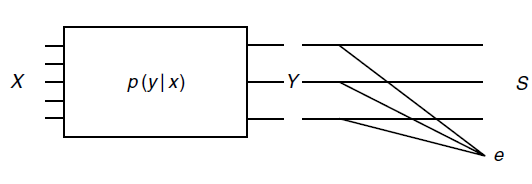
\includegraphics[height=4cm]{img/7-1.png}
    \caption{Erasure Channel}
    \label{fig:ex5}
  \end{figure}
  }
  \begin{solution}
  \begin{equation}
    \begin{aligned}
      I(X;S) &= H(S) -H(S|X) \\
      &= H(S) - \sum_{x\in\mathcal{X}} p(x) \left( \left(\sum_{y\in\mathcal{Y}} \bar{\alpha} p(y|x) \log \bar{\alpha} p(y|x)\right) - \alpha \log \alpha \right) \\
      &= H(S) - \sum_{x\in\mathcal{X}} p(x) \left(\sum_{y\in\mathcal{Y}} \bar{\alpha} p(y|x) \left( \log \bar{\alpha} + \log p(y|x) \right)\right) - \alpha \log \alpha  \\
      &= H(S) - \sum_{x\in\mathcal{X}} p(x) \sum_{y\in\mathcal{Y}} \bar{\alpha} p(y|x)  \log p(y|x) - \alpha \log \alpha - \bar{\alpha} \log \bar{\alpha} \\
      &= H(S) - H(\alpha) -  (1-\alpha) H(Y|X) \\
      &= - \sum_{y\in\mathcal{Y}} \bar{\alpha}p(y) \log \bar{\alpha}p(y) - \alpha\log\alpha - H(\alpha) -  (1-\alpha) H(Y|X) \\
      &= - \sum_{y\in\mathcal{Y}} \bar{\alpha}p(y) \left( \log \bar{\alpha} + \log p(y) \right)  - \alpha\log\alpha - H(\alpha) -  (1-\alpha) H(Y|X) \\
      &= - \sum_{y\in\mathcal{Y}} \bar{\alpha} p(y)  \log p(y) -\bar{\alpha}\log\bar{\alpha} - \alpha\log\alpha - H(\alpha) -  (1-\alpha) H(Y|X) \\
      &= (1-\alpha) H(Y) + H(\alpha)  - H(\alpha)  -  (1-\alpha) H(Y|X)  \\
      &= (1-\alpha) I(X;Y)
    \end{aligned}
  \end{equation}
  Therefore the capacity of this channel is $(1-\alpha)C$.
  \end{solution}
  \label{ex7-5}
\end{exercise}

%%%%%%%%%%%%%%%%%%%%%%%%%%%%%%%%%%%%%%%%%%
%%%%%%%%%%%%%                 %%%%%%%%%%%%
%%%%%%%%%%%%%    EXERCISE 6   %%%%%%%%%%%%
%%%%%%%%%%%%%                 %%%%%%%%%%%%
%%%%%%%%%%%%%%%%%%%%%%%%%%%%%%%%%%%%%%%%%%
\begin{exercise}[Choice of channels]{Find the capacity $C$ of the union of two channels $\left(\mathcal{X}_{1}, p_{1}\left(y_{1} | x_{1}\right), \mathcal{Y}_{1}\right)$ and $\left(\mathcal{X}_{2},\right.$ $\left. p_{2}\left(y_{2} | x_{2}\right), \mathcal{Y}_{2}\right),$ where at each   time, one can send a symbol over channel 1 or channel 2 but not both. Assume that the output alphabets are distinct and do not intersect.
  \begin{enumerate}
    \item Show that $2^{C}=2^{C_{1}}+2^{C_{2}} .$ Thus, $2^{C}$ is the effective alphabet size of a channel with capacity $C$
    \item Compare with Problem 2.10 where $2^{H}=2^{H_{1}}+2^{H_{2}}$, and interpret part (a) in terms of the effective number of noise-free symbols.
    \item Use the above result to calculate the capacity of the following channel.
  \end{enumerate}
  \begin{figure}[H]
    \centering
    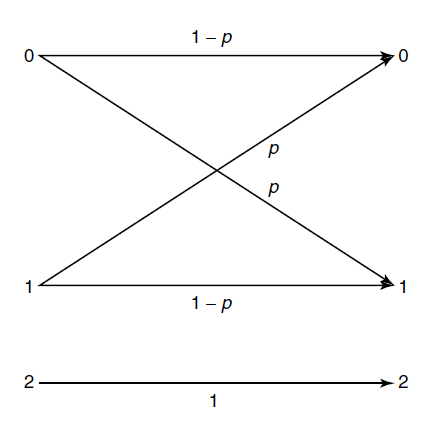
\includegraphics[height=6cm]{img/7-2.png}
    \caption{Choice of Channels}
    \label{fig:ex6}
  \end{figure}
  
  }
  \begin{solution}
  \par{~}
  \begin{enumerate}
    \item { We assume
    \begin{equation}
      p(X=x) = \left\{ \begin{array}{l}
        \pi, x=X_1 \\
        1-\pi, x=X_2
      \end{array}\right.
    \end{equation}
    \begin{equation}
      \begin{aligned}
        I(X,Y) &= H(X) - H(X|Y) \\
        &= - \sum_{x\in \mathcal{X_1 \cup X_2}} p_{X}(x)\log p_{X}(x) - \pi H(X_1|Y_1) - \bar{\pi}H(X_2|Y_2) \\
        &= - \sum_{x\in \mathcal{X_1}} \pi p_{X_1}(x) \log \pi p_{X_1}(x) - \sum_{x\in \mathcal{X_2}} \bar{\pi} p_{X_2}(x) \log \bar{\pi} p_{X_2}(x)  - \pi H(X_1|Y_1) - \bar{\pi}H(X_2|Y_2) \\
        &= H(\pi) + \pi H(X_1) + \bar{\pi} H(X_2) - - \pi H(X_1|Y_1) - \bar{\pi}H(X_2|Y_2) \\
        &= H(\pi) + \pi I(X_1;Y_1) + \bar{\pi} I(X_2;Y_2) \\
        &\le H(\pi) + \pi C_1  + \bar{\pi} C_2
      \end{aligned}
    \end{equation}
    The equality holds when $p(x_1)$ and $p(x_2)$ are at their optimal distribution. We take the derivative on $\pi$ to calculate the capacity.
    \begin{equation}
      \begin{aligned}
        \frac{dI(X;Y)}{d\pi} &= - \log \pi + \log (1-\pi) + C_1 - C_2 := 0\\
        \frac{\pi^{*}}{1-\pi^{*}} &= 2^{C_1-C_2} \\
        \pi^{*} &= \frac{2^{C_1}}{2^{C_1}+2^{C_2}} \\
        \Rightarrow C &= \log (2^{C_1}+2^{C_2})
      \end{aligned}
    \end{equation}
    It follows that $2^C = 2^{C_1} + 2^{C_2}$
    }
    \item { Using the same notion as Assignment3.7, $2^C$ is the effective number of noise-free symbols. Since the two channels are disjoint in their alphabets, the noise-free symbols will also not overlap. Hence the combined capacity is equal to the sum of two sub-channels' noise-free symbols, i.e.  $2^C = 2^{C_1} + 2^{C_2}$}
    \item { From the Binary Symmetric Channel we know that $C_1 = 1 - H(p)$. $C_2 = 0$. Hence we have $C = \log (2^{1-H(p)} +1)$
    }
  \end{enumerate}
  \end{solution}
  \label{ex7-6}
\end{exercise}

%%%%%%%%%%%%%%%%%%%%%%%%%%%%%%%%%%%%%%%%%%
%%%%%%%%%%%%%                 %%%%%%%%%%%%
%%%%%%%%%%%%%    EXERCISE 7   %%%%%%%%%%%%
%%%%%%%%%%%%%                 %%%%%%%%%%%%
%%%%%%%%%%%%%%%%%%%%%%%%%%%%%%%%%%%%%%%%%%
\begin{exercise}[Capacity]{Suppose that channel $\mathcal{P}$ has capacity $C,$ where $\mathcal{P}$ is $m \times n$ channel matrix.
  \begin{enumerate}
    \item What is the capacity of
    $$
    \tilde{\mathcal{P}}=\left[\begin{array}{ll}
    \mathcal{P} & 0 \\
    0 & 1
    \end{array}\right] ?
    $$
    \item  What about the capacity of
    $$
    \hat{\mathcal{P}}=\left[\begin{array}{cc}
    \mathcal{P} & 0 \\
    0 & I_{k}
    \end{array}\right] ?
    $$
    where $I_{k}$ if the $k \times k$ identity matrix.
  \end{enumerate} }
  \begin{solution}
  \par{~}
  \begin{enumerate}
    \item { Note that the new channel is composed of two disjoint sub-channels, $\mathcal{P}$ and a one-to-one channel whose capacity is $1$. By the conclusion of Exercise \ref{ex7-6}, we know that $C_{\mathcal{P}} = \log (2^{C} + 2^{0}) = \log (2^{C} + 1)$. }
    \item { Note that the new channel is composed of two disjoint sub-channels, $\mathcal{P}$ and a one-to-one channel whose capacity is $\log k$. By the conclusion of Exercise \ref{ex7-6}, we know that $C_{\mathcal{P}} = \log (2^{C} + 2^{\log k}) = \log (2^{C} + k)$. }
  \end{enumerate}
  \end{solution}
  \label{ex7-7}
\end{exercise}

%%%%%%%%%%%%%%%%%%%%%%%%%%%%%%%%%%%%%%%%%%
%%%%%%%%%%%%%                 %%%%%%%%%%%%
%%%%%%%%%%%%%    EXERCISE 8   %%%%%%%%%%%%
%%%%%%%%%%%%%                 %%%%%%%%%%%%
%%%%%%%%%%%%%%%%%%%%%%%%%%%%%%%%%%%%%%%%%%
\begin{exercise}[Channel with memory]{ Consider the discrete memoryless channel $Y_{i}=Z_{i} X_{i}$ with input alphabet $X_{i} \in\{-1,1\}$
  \begin{enumerate}
    \item What is the capacity of this channel when $\left\{Z_{i}\right\}$ is i.i.d. with
    $$
    Z_{i}=\left\{\begin{aligned}
    1, & p=0.5 \\
    -1, & p=0.5 ?
    \end{aligned}\right.
    $$
    Now consider the channel with memory. Before transmission begins, $Z$ is randomly chosen and fixed for all time. Thus, $Y_{i}=Z X_{i}$
    \item  What is the capacity if
    $$
    Z=\left\{\begin{aligned}
    1, & p=0.5 \\
    -1, & p=0.5 ?
    \end{aligned}\right.
    $$
  \end{enumerate}  }
  \begin{solution}
  \par{~}
  \begin{enumerate}
    \item { The channel can be modeled as a binary symmetric channel with false rate 0.5, hence the capacity is $1-H(0.5) = 0$.}
    \item { Since $Z$ is fixed for all time, we can set $X_0$ to be 1, and use $Y_i$ to determine what $Z$ is. Then for the rest of the transmissions, $Y$ becomes a function of $X$. Therefore the capacity will approach $\log |\mathcal{X}| = 1$ as $n \rightarrow \infty$. }
  \end{enumerate}
  \end{solution}
  \label{ex7-8}
\end{exercise}

%%%%%%%%%%%%%%%%%%%%%%%%%%%%%%%%%%%%%%%%%%
%%%%%%%%%%%%%                 %%%%%%%%%%%%
%%%%%%%%%%%%%    EXERCISE 9   %%%%%%%%%%%%
%%%%%%%%%%%%%                 %%%%%%%%%%%%
%%%%%%%%%%%%%%%%%%%%%%%%%%%%%%%%%%%%%%%%%%
\begin{exercise}[Tall, fat people]{Suppose that the average height of people in a room is 5 feet. Suppose that the average weight is 100 lb.
  \begin{enumerate}
    \item Argue that no more than one-third of the population is 15 feet tall.
    \item Find an upper bound on the fraction of 300 -Ib 10 -footers in the room.
  \end{enumerate} }
  \begin{solution}
  \par{~}
  \begin{enumerate}
    \item { The height of people can be regarded as a random variable $X$. By Markov’s inequality,
    $$\operatorname{Pr}\{X \geq 15\} \leq \frac{5}{15} = \frac{1}{3}$$
    }
    \item { The weight of people can be regarded as a random variable $Y$. By Markov’s inequality,
    $$\operatorname{Pr}\{Y \geq 300\} \leq \frac{100}{300} = \frac{1}{3}$$}
    and that
    $$\operatorname{Pr}\{X \geq 10\} \leq \frac{5}{10} = \frac{1}{2}$$
    Hence there are at most $\frac{1}{3}$ 300-lb, 10-footers among all the people.
  \end{enumerate}
  \end{solution}
  \label{ex7-9}
\end{exercise}

\section{Differential Entropy}
%%%%%%%%%%%%%%%%%%%%%%%%%%%%%%%%%%%%%%%%%%
%%%%%%%%%%%%%                 %%%%%%%%%%%%
%%%%%%%%%%%%%    EXERCISE 1   %%%%%%%%%%%%
%%%%%%%%%%%%%                 %%%%%%%%%%%%
%%%%%%%%%%%%%%%%%%%%%%%%%%%%%%%%%%%%%%%%%%
\begin{exercise}[Differential entropy]{Evaluate the differential entropy $h(X)=$ $-\int f \ln f$ for the following:
  \begin{enumerate}
    \item The exponential density, $f(x)=\lambda e^{-\lambda x}, x \geq 0$
    \item The Laplace density, $f(x)=\frac{1}{2} \lambda e^{-\lambda|x|}$
    \item The sum of $X_{1}$ and $X_{2},$ where $X_{1}$ and $X_{2}$ are  independent normal random variables with means $\mu_{i}$ and variances $\sigma_{i}^{2}, i= 1,2$
  \end{enumerate}}
  \begin{solution}
  \par{~}
  \begin{enumerate}
    \item \begin{equation}
      \begin{aligned}
        h(X) &= -\int _{0}^{\infty} \lambda e^{-\lambda x} \ln \lambda e^{-\lambda x} dx\\
        &= -\int _{0}^{\infty} \lambda e^{-\lambda x} (\ln \lambda  - \lambda x) dx\\
        &= \ln \lambda \int _{0}^{\infty} e^{-\lambda x}   d (- \lambda x) -  \lambda  \int _{0}^{\infty} x  d  e^{-\lambda x} \\
        &= \ln \lambda e^{-\lambda x}  \bigg| _{0} ^{\infty} - \lambda x e^{-\lambda x} \bigg| _{0} ^{\infty} - \int_{0}^{\infty} e^{-\lambda x} d (-\lambda x) \\
        &= - \ln \lambda + 1 = \ln \frac{e}{\lambda}
      \end{aligned}
    \end{equation}
    \item \begin{equation}
      \begin{aligned}
        h(X) &= - \int_{-\infty}^{+\infty} \frac{1}{2} \lambda e^{-\lambda |x|} \ln \frac{1}{2} \lambda e^{-\lambda |x|} dx \\
        &= - 2 \int_{0}^{+\infty} \frac{1}{2}\lambda e^{-\lambda x} \ln \frac{1}{2}\lambda e^{-\lambda x}  dx \\
        &= - \int_{0}^{+\infty} \lambda e^{-\lambda x} \ln \lambda e^{-\lambda x} dx +  \ln 2 \int_{0}^{\infty} \lambda e^{-\lambda x} dx \\
        &= \ln \frac{e}{\lambda} - \ln 2 \cdot e^{-\lambda x} \bigg| ^{\infty}_{0} \\
        &= \ln \frac{2e}{\lambda}
      \end{aligned}
    \end{equation}
    \item By condition we know that
    \begin{equation}
      X_1, X_2 \sim \mathcal{N}\left(
        \left[\begin{array}{cc}
          \mu_1 & \mu_2 
        \end{array}\right], 
        \left[\begin{array}{cc}
          \sigma_1^{2} & 0 \\
           0 & \sigma_2^{2}
        \end{array}\right]\right)
    \end{equation}
    Since $X_1 + X_2 = \left[\begin{array}
      {cc} X_1 & X_2
    \end{array}\right] \left[\begin{array}
      {c} 1 \\ 1
    \end{array}\right]$, it follows that $X_1 + X_2 \sim \mathcal{N} (\mu_1 + \mu_2, \sigma_{1}^{2} + \sigma_{2}^{2})$.
    \begin{equation}
      \begin{aligned}
        f(x) &= \frac{1}{\sqrt{2 \pi (\sigma_{1}^{2} + \sigma_{2}^{2})}} e^{-\frac{(x-(\mu_1 + \mu_2))^{2}}{2 (\sigma_{1}^{2} + \sigma_{2}^{2})}} \\        
        h(X)&=-\int f(x) \log f(x) d x \\
        &=-\int f(x) \log \frac{1}{\sqrt{2 \pi (\sigma_{1}^{2} + \sigma_{2}^{2})}}+f(x)\left(-\frac{(x-(\mu_1 + \mu_2))^{2}}{2 (\sigma_{1}^{2} + \sigma_{2}^{2})}\right) d x         
        \end{aligned}      
    \end{equation}
    By property of normal distribution, we have
    \begin{equation}
      \int f(x) d x=1 \text { and } \int(x-(\mu_1 + \mu_2))^{2} f(x) d x=\sigma_{1}^{2} + \sigma_{2}^{2}
    \end{equation}
    Hence, 
    \begin{equation}
      h(X) = \frac{1}{2} \log 2\pi (\sigma_{1}^{2}+\sigma_{2}^{2}) + \frac{1}{2}
    \end{equation}
  \end{enumerate}
  \end{solution}
  \label{ex1}
\end{exercise}

%%%%%%%%%%%%%%%%%%%%%%%%%%%%%%%%%%%%%%%%%%
%%%%%%%%%%%%%                 %%%%%%%%%%%%
%%%%%%%%%%%%%    EXERCISE 2   %%%%%%%%%%%%
%%%%%%%%%%%%%                 %%%%%%%%%%%%
%%%%%%%%%%%%%%%%%%%%%%%%%%%%%%%%%%%%%%%%%%
\begin{exercise}[Concavity of determinants]{ Let $K_{1}$ and $K_{2}$ be two symmetric nonnegative definite $n \times n$ matrices. Prove:
  $$
  \left|\lambda K_{1}+\bar{\lambda} K_{2}\right| \geq\left|K_{1}\right|^{\lambda}\left|K_{2}\right|^{\bar{\lambda}} \quad \text { for } 0 \leq \lambda \leq 1, \quad \bar{\lambda}=1-\lambda
  $$
  where $|K|$ denotes the determinant of $K .$ [Hint: Let $\mathbf{Z}=\mathbf{X}_{\theta}$ where $\mathbf{X}_{1} \sim N\left(0, K_{1}\right), \mathbf{X}_{2} \sim N\left(0, K_{2}\right)$ and $\theta=$ Bernoulli $(\lambda) .$ Then
  use $h(\mathbf{Z} | \theta) \leq h(\mathbf{Z}) .]$}
  \begin{proof}
  Let $Z = \theta X_1 + (1 - \theta) X_2$, where $\theta,X_1$ and $X_2$ are independent, $\mathbf{X}_{1} \sim N\left(0, K_{1}\right), \mathbf{X}_{2} \sim N\left(0, K_{2}\right)$ and $\theta=$ Bernoulli $(\lambda) .$ Note that for every entry in the covariance matrix of $Z$,
  \begin{equation}
    \begin{aligned}
      cov(Z_i,Z_j) &= E(Z_i Z_j) E((\theta X_{1i} + \bar{\theta} X_{2i})(\theta X_{1j} + \bar{\theta} X_{2j})) \\
      &= E(\theta^2) E X_{1i} X_{1j} + E(\bar{\theta}^2) E X_{2i} X_{2j} \\
      &= \lambda cov(X_{1i},X_{1j}) + \bar{\lambda} cov (X_{2i},X_{2j})
    \end{aligned}
  \end{equation}
  Hence we have $K_Z = \lambda K_{X_1} + \bar{\lambda} K_{X_2}$. Also note that $EZ = \mathbf{0}$. By Theorem 8.6.5 [Cover] we have that 
  \begin{equation}
    h(Z) \le \frac{1}{2} \log (2\pi e)^n \left| K_Z \right| = \frac{1}{2} \log (2\pi e)^n \left|  \lambda K_{1} + \bar{\lambda} K_{2} \right|
    \label{eqn:1}
  \end{equation}
  By the formula for entropy of a multivariate normal distribution, we have that
  \begin{equation}
    \begin{aligned}
      h(X_1) &\le \frac{1}{2} \log (2\pi e)^n \left| K_1 \right| \\
      h(X_2) &\le \frac{1}{2} \log (2\pi e)^n \left| K_2 \right| \\
      \Rightarrow h(Z|\theta) &= \lambda h(X_1) + \bar{\lambda}h(X_2) \\
      &=  \frac{\lambda}{2} \log (2\pi e)^n \left| K_1 \right| + \frac{\bar{\lambda}}{2} \log (2\pi e)^n \left| K_2 \right| \\
      &= \frac{1}{2} \log (2\pi e)^n \left| K_{1} \right|^{\lambda} \left| K_{2} \right|^{\bar{\lambda}}
    \end{aligned}
    \label{eqn:2}
  \end{equation}
  Note that $h(Z|\theta) \le h(Z)$. The result follows from Equation \ref{eqn:1} and \ref{eqn:2}.
  \end{proof}
  \label{ex2}
\end{exercise}

%%%%%%%%%%%%%%%%%%%%%%%%%%%%%%%%%%%%%%%%%%
%%%%%%%%%%%%%                 %%%%%%%%%%%%
%%%%%%%%%%%%%    EXERCISE 3   %%%%%%%%%%%%
%%%%%%%%%%%%%                 %%%%%%%%%%%%
%%%%%%%%%%%%%%%%%%%%%%%%%%%%%%%%%%%%%%%%%%
\begin{exercise}[Uniformly distributed noise]{ Let the input random variable $X$ to a channel be uniformly distributed over the interval $-\frac{1}{2} \leq x \leq+\frac{1}{2}$ Let the output of the channel be $Y=X+Z,$ where the noise random variable is uniformly distributed over the interval $-a / 2 \leq z \leq$ $+a / 2$
  \begin{enumerate}
    \item Find $I(X ; Y)$ as a function of $a$
    \item For $a=1$ find the capacity of the channel when the input $X$ is peak-limited; that is, the range of $X$ is limited to $-\frac{1}{2} \leq x \leq$ $+\frac{1}{2} .$ What probability distribution on $X$ maximizes the mutual information $I(X ; Y) ?$
    \item (Optional) Find the capacity of the channel for all values of $a$, again assuming that the range of $X$ is limited to $-\frac{1}{2} \leq x \leq+\frac{1}{2}$
  \end{enumerate} }
  \begin{solution}
  \par{~}
  \begin{enumerate}
    \item We first calculate the distribution of $Y$.
    \begin{equation}
      p_Y (y) = \int_{-\frac{a}{2}}^{\frac{a}{2}} \frac{1}{a} \mathbf{1}_{\left\{ y - \frac{1}{2} \le z \le y + \frac{1}{2} \right\}} d z
    \end{equation}
    If $a\le 1$, we have that
    \begin{equation}
      p_Y (y) = \begin{cases}
        \frac{1}{a} \left( y + \frac{a+1}{2}\right)  & -\frac{a+1}{2} \le y \le \frac{a-1}{2} \\
        1 & \frac{a-1}{2} < y \le \frac{1-a}{2} \\
        \frac{1}{a} \left(-y + \frac{a+1}{2}\right) & \frac{1-a}{2} < y \le \frac{a+1}{2}
      \end{cases}
    \end{equation}
    If $a > 1$, we have that
    \begin{equation}
      p_Y (y) = \begin{cases}
        \frac{1}{a} \left( y + \frac{a+1}{2}\right)  & -\frac{a+1}{2} \le y \le \frac{1-a}{2} \\
        \frac{1}{a} & \frac{1-a}{2} < y \le \frac{a-1}{2} \\
        \frac{1}{a} \left(-y + \frac{a+1}{2}\right) & \frac{a-1}{2} < y \le \frac{a+1}{2}
      \end{cases}
    \end{equation}
    For $a \le 1$,
    \begin{equation}
      \begin{aligned}
        I(X;Y) &= h(Y) - h(Y|X) = h(Y) - h(Z) = h(Y) - \ln a \\
        &= \int_{-\frac{a+1}{2}}^{\frac{a+1}{2}} p(y) \ln p(y) dy - \ln a \\
        &= - 2 \int_{0}^{\frac{1-a}{2}} 1 \ln 1 dy - 2 \int_{\frac{1-a}{2}}^{\frac{1+a}{2}} \frac{1}{a} (-y + \frac{a+1}{2}) \log \frac{1}{a} (-y + \frac{a+1}{2}) dy - \ln a \\
        &= 0 - 2a \int_{0}^{1} t \ln t dt - \ln a \quad ( t \triangleq \frac{1}{a}\left(-y + \frac{a+1}{2})\right) \\
        &= - 2a \left( \frac{1}{2} t^2 \ln t - \frac{1}{4} t^2 \right) \bigg|_{0}^{1} - \ln a \\
        &= \frac{a}{2} - \ln a
      \end{aligned}
    \end{equation}
    For $a > 1$,
    \begin{equation}
      \begin{aligned}
        I(X;Y) &= h(Y) - h(Y|X) = h(Y) - h(Z) = h(Y) - \ln a \\
        &= \int_{-\frac{a+1}{2}}^{\frac{a+1}{2}} p(y) \ln p(y) dy - \ln a \\
        &= - 2 \int_{0}^{\frac{a-1}{2}} \frac{1}{a} \ln \frac{1}{a} dy - 2 \int_{\frac{a-1}{2}}^{\frac{1+a}{2}} \frac{1}{a} (-y + \frac{a+1}{2}) \log \frac{1}{a} (-y + \frac{a+1}{2}) dy - \ln a \\
        &= \frac{a-1}{a} \ln a - 2a \int_{0}^{\frac{1}{a}} t \ln t dt - \ln a \quad ( t \triangleq \frac{1}{a}\left(-y + \frac{a+1}{2})\right) \\
        &= - \frac{1}{a} \ln a - 2a \left( \frac{1}{2} t^2 \ln t - \frac{1}{4} t^2 \right) \bigg|_{0}^{\frac{1}{a}}\\
        &= \frac{1}{2a}
      \end{aligned}
    \end{equation}
    \item Since $X$ and $Z$ are both limited to $\left[-\frac{1}{2},\frac{1}{2}\right]$, $Y$ is limited to $\left[-1,1\right]$. By the Example 12.2.4 in [Cover], the maximal differential entropy $h(Y)$ is $\ln 2$, which can be obtained when $Y$ is uniformly distributed, and thus $p(X = -\frac{1}{2}) = p(X = \frac{1}{2}) = \frac{1}{2}$.
    \begin{equation}
      I(X;Y) = h(Y) - h(Y|X) = h(Y) - h(Z) = h(Y) - \ln 1 \le \ln 2 \text{ nats}
    \end{equation}
    The capacity is $\ln 2$ nats $= 1$ bit.
    \item If $a = \frac{1}{k}, k\in \mathbf{N}$, then we can construct $X$ to be uniformly distributed on $\left\{-\frac{1}{2}, -\frac{1}{2} + \frac{1}{k}, \ldots,\frac{1}{2} \right\}$, with $Y$ uniformly distributed on $\left[-\frac{1}{2}-\frac{1}{2k}, -\frac{1}{2}+\frac{1}{2k} \right]$. In this case, the maximal mutual information can be obtained. $C = \log \left(1+ \frac{1}{k}\right)$.
  \end{enumerate}
  \end{solution}
  \label{ex3}
\end{exercise}


%%%%%%%%%%%%%%%%%%%%%%%%%%%%%%%%%%%%%%%%%%
%%%%%%%%%%%%%                 %%%%%%%%%%%%
%%%%%%%%%%%%%    EXERCISE 4   %%%%%%%%%%%%
%%%%%%%%%%%%%                 %%%%%%%%%%%%
%%%%%%%%%%%%%%%%%%%%%%%%%%%%%%%%%%%%%%%%%%
\begin{exercise}[Channel with uniformly distributed noise]{ Consider a additive channel whose input alphabet $\mathcal{X}=\{0,\pm 1,\pm 2\}$ and whose output $Y=X+Z,$ where $Z$ is distributed uniformly over the interval $[-1,1] .$ Thus, the input of the channel is a discrete random variable, whereas the output is continuous. Calculate the capacity $C=$ $\max _{p(x)} I(X ; Y)$ of this channel.}
  \begin{solution}
  Note that
  \begin{equation}
    I(X;Y) = h(Y) - h(Y|X) = h(Y) -h(Z) = h(Y) - \log 2
  \end{equation}
  Note that the support set of $Y$ is $\left[-3,3\right]$.By the Example 12.2.4 in [Cover], the maximal differential entropy $h(Y)$ is $\log 6$, which can be obtained when $p(X=-2) = p(X=0) = p(X=2) = \frac{1}{3}$, and $Y$ is uniformly distributed. The maximal mutual information is $\log 3$.
  \end{solution}
  \label{ex4}
\end{exercise}


%%%%%%%%%%%%%%%%%%%%%%%%%%%%%%%%%%%%%%%%%%
%%%%%%%%%%%%%                 %%%%%%%%%%%%
%%%%%%%%%%%%%    EXERCISE 5   %%%%%%%%%%%%
%%%%%%%%%%%%%                 %%%%%%%%%%%%
%%%%%%%%%%%%%%%%%%%%%%%%%%%%%%%%%%%%%%%%%%


\begin{lemma}[Conditional Expectation of Two Normal Random Variables] {Let $X$ and $Y$ be jointly Gaussian with variances $\sigma_1^2$ ,$\sigma_2^2$ and correlation coefficient $\rho$. We have that $E(X|Y) = \frac{\sigma_1 \rho}{\sigma_2} Y$.}
  \begin{proof}
    We calculate the conditional probability density of $p(x|y)$
    \begin{equation}
      \begin{aligned}
        p(x|y) &= \frac{p(x,y)}{p(y)} \\
        &= \frac{\frac{1}{2\pi \sqrt{1-\rho^2}\sigma_1\sigma_2} \operatorname{exp}\left\{-\frac{1}{2(1-\rho^2)}\left[\frac{x^2}{\sigma_1^2}-2\rho\frac{xy}{\sigma_1\sigma_2}+\frac{y^2}{\sigma_2^2}\right]\right\}}{\frac{1}{\sqrt{2\pi}\sigma_2}\operatorname{exp} \left\{ - \frac{1}{2} \frac{y^2}{\sigma_2^2}\right\} }  \\
        &= \frac{1}{\sqrt{2\pi (1-\rho^2)}} \operatorname{exp} \left\{ -\frac{1}{2(1-\rho^2)}\left[\frac{x^2}{\sigma_1^2}-2\rho\frac{xy}{\sigma_1\sigma_2}+\frac{\rho^2 y^2}{\sigma_2^2}\right] -\frac{1}{2} \frac{y^2}{\sigma_2^2}  +\frac{1}{2} \frac{y^2}{\sigma_2^2}   \right\} \\
        &= \frac{1}{\sqrt{2\pi (1-\rho^2)}} \operatorname{exp} \left\{ -\frac{1}{2(1-\rho^2)\sigma_1^2}\left(x - \frac{\sigma_1 \rho y}{\sigma_2}\right)   \right\}
      \end{aligned}
    \end{equation}
    With $Y$ given, the mean value is $\frac{\sigma_1 \rho}{\sigma_2} Y$
  \end{proof}
\end{lemma}


\begin{exercise}[Gaussian mutual information]{Suppose that $(X, Y, Z)$ are jointly Gaussian and that $X \rightarrow Y \rightarrow Z$ forms a Markov chain. Let $X$ and $Y$ have correlation coefficient $\rho_{1}$ and let $Y$ and $Z$ have correlation coefficient $\rho_{2} .$ Find $I(X ; Z)$}
  \begin{solution} By the formula of mutual information between correlated Gaussian random variables, we have
    \begin{equation}
      I(X;Z) = -\frac{1}{2} \log (1-\rho_{xz} ^2)
    \end{equation}

  With the lemma above, we can derive $\rho_{xz}$ as follows.

  \begin{equation}
      \begin{aligned}
      \rho_{x z} &=\frac{\mathrm{E}\{X Z\}}{\sigma_{x} \sigma_{z}} \\
      &=\frac{\mathrm{E}\{\mathrm{E}\{X Z | Y\}\}}{\sigma_{x} \sigma_{z}} &\quad {\text{Nested Expectation}} \\
      &=\frac{\mathrm{E}\{\mathrm{E}\{X | Y\} \mathrm{E}\{Z | Y\}\}}{\sigma_{x} \sigma_{z}} &\quad {\text{Markov Chains}}\\
      &=\frac{\mathrm{E}\left\{\left(\frac{\sigma_{x} \rho_{x y}}{\sigma_{y}} Y\right)\left(\frac{\sigma_{z} \rho_{z x}}{\sigma_{y}} Y\right)\right\}}{\sigma_{x} \sigma_{z}} &\quad {\text{Apply the Lemma}} \\
      &=\rho_{x y} \rho_{z y}
      \end{aligned}
  \end{equation}
  Hence $I(X;Z) = -\frac{1}{2} \log (1 -\rho_{x y}^2 \rho_{z y}^2 )$
  \end{solution}
  \label{ex5}
\end{exercise}

\section{Gaussian Channel}
%%%%%%%%%%%%%%%%%%%%%%%%%%%%%%%%%%%%%%%%%%
%%%%%%%%%%%%%                 %%%%%%%%%%%%
%%%%%%%%%%%%%    EXERCISE 1   %%%%%%%%%%%%
%%%%%%%%%%%%%                 %%%%%%%%%%%%
%%%%%%%%%%%%%%%%%%%%%%%%%%%%%%%%%%%%%%%%%%
\begin{exercise}[Channel with two independent looks at $Y$]{ Let $Y_{1}$ and $Y_{2}$ be conditionally independent and conditionally identically distributed given $X$
  \begin{enumerate}
    \item Show that $I\left(X ; Y_{1}, Y_{2}\right)=2 I\left(X ; Y_{1}\right)-I\left(Y_{1} ; Y_{2}\right)$
    \item Conclude that the capacity of the channel $X\mapsto Y_1,Y_2$ is less than twice the capacity of the channel $X \mapsto Y_1$.
  \end{enumerate}}
  \begin{proof}
  \par{~}
  \begin{enumerate}
    \item {
      \begin{equation}
        \begin{aligned}
          I(X;Y_1,Y_2) &= H(Y_1,Y_2) - H(Y_1,Y_2|X) \\
          &= H(Y_1,Y_2) - H(Y_1|X) - H(Y_2|X) \\
          &= H(Y_1) + H(Y_2) - I(Y_1;Y_2) -  H(Y_1|X) - H(Y_2|X) \\
          &=I(X;Y_1) + I(X;Y_2)- I(Y_1,Y_2) \\
          &= 2I(X;Y_1) - I(Y_1,Y_2)
        \end{aligned}
      \end{equation}
     }
    \item { 
\begin{equation}
  \begin{aligned}
    C_1 &= \max_{p(x)} I(X;Y_1,Y_2) \\
    &= \max_{p(x)} (2I(X;Y_1) - I(Y_1,Y_2)) \\
    &\le \max_{p(x)} 2I(X;Y_1) \\
    &= 2C_2
  \end{aligned}
\end{equation}
    }
  \end{enumerate}
  \end{proof}
  \label{ex1}
\end{exercise}

%%%%%%%%%%%%%%%%%%%%%%%%%%%%%%%%%%%%%%%%%%
%%%%%%%%%%%%%                 %%%%%%%%%%%%
%%%%%%%%%%%%%    EXERCISE 2   %%%%%%%%%%%%
%%%%%%%%%%%%%                 %%%%%%%%%%%%
%%%%%%%%%%%%%%%%%%%%%%%%%%%%%%%%%%%%%%%%%%
\begin{exercise}[Two-look Gaussian channel]{ Given $X \mapsto Y_1,Y_2$. Consider the ordinary Gaussian channel with two correlated looks at ${X},$ that is, $Y=\left(Y_{1}, Y_{2}\right),$ where
  $$
  \begin{aligned}
  Y_{1} &=X+Z_{1} \\
  Y_{2} &=X+Z_{2}
  \end{aligned}
  $$
  with a power constraint $P$ on $X,$ and $\left(Z_{1}, Z_{2}\right) \sim \mathcal{N}_{2}(0, K),$ where
$$
K=\left[\begin{array}{ll}
N & N \rho \\
N \rho & N
\end{array}\right]
$$
Find the capacity $C$ for
\begin{enumerate}
  \item $\rho=1$
  \item $\rho=0$
  \item $\rho=-1$
\end{enumerate}}
  \begin{solution}
  \par{~}
  From Theorem 8.6.5 [Cover] we know that the Gaussian distribution maximizes the entropy over all distributions with the same variance. Hence it is clear that normally distributed $X \sim \mathcal{N}(0,P)$ will maximize the mutual information. In this case $(Y_1,Y_2) \sim \left(0, \left[\begin{array}{cc}
    P+N & P+\rho N \\
    P +\rho N & P + N
  \end{array}\right]\right)$
  \begin{equation}
    \begin{aligned}
      \max I(X;Y_1,Y_2) &= h(Y_1,Y_2) - h(Y_1,Y_2|X) \\
      &= h(Y_1,Y_2) - h(Z_1,Z_2) \\
      &= \frac{1}{2} \log \left(2\pi e\right)^2 \left|\begin{array}{cc}
        P+N & P+\rho N \\
        P +\rho N & P + N
      \end{array} \right| - \frac{1}{2} \log \left(2\pi e\right)^2 \left| \begin{array}{ll}
        N & N \rho \\
        N \rho & N
        \end{array}  \right| \\
      &= \frac{1}{2} \log \left(1 + \frac{2P}{(1+\rho)N}\right)
    \end{aligned}
  \end{equation}
  \begin{enumerate}
    \item $\rho = 1$, $C = \frac{1}{2} \log \left(1 + \frac{P}{N}\right)$
    \item $\rho = 0$, $C = \frac{1}{2} \log \left(1 + \frac{2P}{N}\right)$
    \item $\rho = -1$, $C = +\infty$.
  \end{enumerate}
  \end{solution}
  \label{ex2}
\end{exercise}


%%%%%%%%%%%%%%%%%%%%%%%%%%%%%%%%%%%%%%%%%%
%%%%%%%%%%%%%                 %%%%%%%%%%%%
%%%%%%%%%%%%%    EXERCISE 3   %%%%%%%%%%%%
%%%%%%%%%%%%%                 %%%%%%%%%%%%
%%%%%%%%%%%%%%%%%%%%%%%%%%%%%%%%%%%%%%%%%%
\begin{exercise}[Output power constraint]{ Consider an additive white Gaussian noise channel with an expected output power constraint $P .$ Thus, $Y=X+Z, Z \sim N\left(0, \sigma^{2}\right), Z$ is independent of $X,$ and $E Y^{2} \leq P$ Find the channel capacity.}
  \begin{solution}
  \begin{equation}
    \begin{aligned}
      I(X;Y) &= h(Y) - h(Y|X) \\
      &= h(Y) - h(Z) \\
      &= h(Y) - \frac{1}{2}\log \left(2 \pi e \sigma^2\right) \\
      &\le \frac{1}{2} \log \left( 2 \pi e P \right)  - \frac{1}{2}\log \left(2 \pi e \sigma^2\right)  \\
      &= \frac{1}{2} \log \frac{P}{\sigma^2}
    \end{aligned}
  \end{equation}
  The equailty holds when $Y$ is normally distributed. In this case $X \sim \mathcal{N} (0,P-\sigma^2)$.
  \end{solution}
  \label{ex3}
\end{exercise}

%%%%%%%%%%%%%%%%%%%%%%%%%%%%%%%%%%%%%%%%%%
%%%%%%%%%%%%%                 %%%%%%%%%%%%
%%%%%%%%%%%%%    EXERCISE 4   %%%%%%%%%%%%
%%%%%%%%%%%%%                 %%%%%%%%%%%%
%%%%%%%%%%%%%%%%%%%%%%%%%%%%%%%%%%%%%%%%%%
\begin{exercise}[Exponential noise channels]{ $\quad Y_{i}=X_{i}+Z_{i},$ where $Z_{i}$ is i.i.d. exponentially distributed noise with mean $\mu$. Assume that we have a mean constraint on the signal (i.e., $E X_{i} \leq \lambda$ ). Show that the capacity of such a channel is $C=\log \left(1+\frac{\lambda}{\mu}\right)$}
  \begin{proof}
  \begin{equation}
    \begin{aligned}
      I(X;Y) &= h(Y) - h(Y|X) \\
      &= h(Y) - h(Z)\\
      &= h(Y) - \sum_i h(Z_i) \\
      &\le \sum_i \left(h(Y_i) - h(Z_i)\right)
    \end{aligned}
  \end{equation}
  The equailty holds when $Y_i$s are independent, which can be obtained if $X_i$s are independent. Hence we can only consider the channel for the input and output to be single-valued. Still, $I(X;Y) = h(Y) - h(Z)$ holds.

  Note for exponentially distributed $Z$,
  \begin{equation}
    \begin{aligned}
      h(Z) &= - \int_{0}^{+\infty} g(z) \ln  \frac{1}{\mu} e^{-\frac{z}{\mu}}  dz \\
      &= - \int_{0}^{+\infty} g(z) \ln  \frac{1}{\mu}   dz - \int_{0}^{+\infty} g(z) \frac{z}{\mu}  dz \\
      &= 1 + \ln \mu 
    \end{aligned}
  \end{equation}

  Note that $EY = EX + EZ \le \lambda + \mu$.  For mean-value bounded $Y$, by Theorem 12.1.1 and Example 12.2.5 [Cover], the maximizing differential entropy is $h^{*}(Y) = 1 + \ln (\lambda + \mu)$, with distribution $p^{*}(y) = \frac{1}{\lambda + \mu} e^{- \frac{y}{\lambda + \mu}}$. Therefore
  \begin{equation}
    I(X;Y) \le \sum_{i=1}^{n} \left(\left(1 + \ln(\lambda + \mu)\right)- \left(1 + \ln(\mu)\right)\right) = n \ln \frac{\lambda + \mu}{\mu}
  \end{equation}

  The equailty holds when $X_i$ are independent with mean value $\lambda$ and $Y_i \sim \text{exp} \left(\frac{1}{\lambda+\mu}\right)$. We need to find such distribution for $X_i$. Since $X_i$ and $Z_i$ are independent and $Y_i = X_i + Z_i$, it follows that the characteristc functions hold the following relation.
  \begin{equation}
    \phi_Y (t) = \phi_X (t) \cdot \phi_Z(t)
  \end{equation}
  Therefore
  \begin{equation}
    \begin{aligned}
      \phi_X (t) &= \frac{\phi_Y(t)}{\phi_Z(t)} \\
      &= \frac{\left(1 - i(\lambda + \mu)t\right)^{-1}}{\left( 1 - i \mu t\right)^{-1}} \\
      &= \frac{1}{\lambda + \mu} \frac{\left[\mu - i \mu (\lambda + \mu)t\right] + \lambda}{1 - i(\lambda + \mu)t} \\
      &= \frac{\mu}{\lambda + \mu} + \frac{\lambda}{\lambda + \mu} \left(1 - i (\lambda + \mu)t\right)^{-1}
    \end{aligned}
  \end{equation}

  The characteristc function above is a linear combination of two kinds of distribution. We can set every $X_i$ to be 0 with the probability of $\frac{\mu}{\lambda + \mu}$, and to be exponentially distributed with mean value $\lambda + \mu$ by the probability of $\frac{\lambda}{\mu + \lambda}$. Then the channel capacity $ n \ln \frac{\lambda + \mu}{\mu} $ can be obtained.

  \end{proof}
  \label{ex4}
\end{exercise}

\end{document}
